\documentclass[twocolumn]{svjour3}          % twocolumn
%
\smartqed  % flush right qed marks, e.g. at end of proof
%
\usepackage{graphicx}
\usepackage{enumerate}
\usepackage{latexsym}
\usepackage{amsfonts}
\usepackage{amsmath}
\usepackage{amssymb}
\usepackage[bigsqcap]{stmaryrd}
\usepackage{color}
\usepackage{colortbl}
\usepackage{epsfig}
\usepackage{xspace}
\usepackage{graphicx}
\usepackage{esvect} % for arrows
\usepackage{subfigure}
\usepackage{balance}
\usepackage{cite}
\usepackage[english]{babel}

%%%%%%%%%%%%%%%%%%%%%%%%%%%%%%%%%%%%%
%% DO NOT DELETE!!
%%%%%%%%%%%%%%%%%%%%%%%%%%%%%%%%%%%%%
%\usepackage{tikz}
%\usetikzlibrary{trees}

\usepackage{multirow}
\usepackage{url}


%%%%%%%%%%%%%%%%%%%%%%%%%%%%%%%%%%%%%%%%%%%%%%%%%%%%%%%%%%
%\newcommand{\eq}{\kw{eq}}

\newcommand{\rE}[1]{\kw{\small eHFD}_{#1}}
\newcommand{\rH}[1]{\kw{\small HFD}_{#1}}
\newcommand{\ab}{\allowbreak}

\sloppy
\newcommand{\rtable}[1]{\ensuremath{\mathsf{#1}}}
\newcommand{\ratt}[1]{\ensuremath{\mathit{#1}}}
\newcommand{\at}[1]{\protect\ensuremath{\mathsf{#1}}\xspace}
\newcommand{\myhrule}{\rule[.5pt]{\hsize}{.5pt}}
\newcommand{\oneurl}[1]{\texttt{#1}}
\newcommand{\eat}[1]{}
\newcommand{\tabstrut}{\rule{0pt}{4pt}\vspace{-0.1in}}
\newcommand{\stab}{\vspace{1.0ex}\noindent}
\newcommand{\sstab}{\vspace{0.5ex}\noindent}
\newcommand{\match}{\rightleftharpoons}
\newcommand{\eg}{\emph{e.g.,}\xspace}
\newcommand{\ie}{\emph{i.e.,}\xspace}
\newcommand{\true}{\kw{true}}
\newcommand{\kop}{\kw{op}}
\newcommand{\nil}{\kw{nil}}
\newcommand{\Op}{\kw{Op}}
\newcommand{\proofs}{\noindent{\bf Proof sketch:\/ }}
\newcommand{\wrt}{\emph{w.r.t.}\xspace}


%%%%%%%%%%%%%%%%%%%%%%%%%%%%%%%%%%%%%%%%%%%%%%%%%%%%%%%%%%%%%%%%%%%%%%%%%%%%%%
% ALGORITHMS
%%%%%%%%%%%%%%%%%%%%%%%%%%%%%%%%%%%%%%%%%%%%%%%%%%%%%%%%%%%%%%%%%%%%%%%%%%%%%%%
\newcommand{\SELECT}{\mbox{{\bf select}}\ }
\newcommand{\FROM}{\mbox{{\bf from}\ }}
\newcommand{\WHERE}{\mbox{\bf where}\ }
\newcommand{\SUM}{\mbox{{\bf sum}}\ }
\newcommand{\GROUPBY}{\mbox{{\bf group by}}\ }
\newcommand{\HAVING}{\mbox{{\bf having}}\ }
\newcommand{\CASE}{\mbox{{\bf case}}\ }
\newcommand{\END}{\mbox{{\bf end}}\ }
\newcommand{\WHEN}{\mbox{{\bf when}}\ }
\newcommand{\EXISTS}{\mbox{{\bf exists}}\ }
\newcommand{\COUNT}{\mbox{\kw{count}}}
\newcommand{\INSERTINTO}{\mbox{{\bf insert into}}\ }
\newcommand{\UPDATE}{\mbox{{\bf update}}\ }
\newcommand{\SET}{\mbox{{\bf set}}\ }
\newcommand{\IN}{\mbox{{\bf in}}\ }
\newcommand{\If}{\mbox{\bf if}\ }
\newcommand{\Upon}{\mbox{\bf upon}\ }
\newcommand{\Send}{\mbox{\bf send}\ }
\newcommand{\Let}{\mbox{\bf let}\ }
\newcommand{\Call}{\mbox{\bf call}\ }
\newcommand{\Then}{\mbox{\bf then}\ }
\newcommand{\To}{\mbox{\bf to}\ }
\newcommand{\Else}{\mbox{\bf else}\ }
\newcommand{\ElseIf}{\mbox{\bf elseif}\ }
\newcommand{\While}{\mbox{\bf while}\ }
\newcommand{\Begin}{\mbox{\bf begin}\ }
\newcommand{\End}{\mbox{\bf end}\ }
\newcommand{\Do}{\mbox{\bf do}\ }
\newcommand{\Downto}{\mbox{\bf downto}\ }
\newcommand{\Repeat}{\mbox{\bf repeat}\ }
\newcommand{\Until}{\mbox{\bf until}\ }
\newcommand{\For}{\mbox{\bf for}\ }
\newcommand{\Each}{\mbox{\bf each}\ }
\newcommand{\Handle}{\mbox{\bf handle}\ }
\newcommand{\ForEach}{\mbox{\bf for each}\ }
\newcommand{\Or}{\mbox{\bf or}\ }
\renewcommand{\And}{\mbox{\bf and}\ }
\newcommand{\Not}{\mbox{\bf not}\ }
\newcommand{\Break}{\mbox{\bf break}\ }
\newcommand{\Continue}{\mbox{\bf continue}\xspace}
\newcommand{\Return}{\mbox{\bf return}\ }
\newcommand{\Case}{\mbox{\bf case}\ }
\newcommand{\Of}{\mbox{\bf of}\ }
\newcommand{\EndCase}{\mbox{\bf end-case}\ }
\newcommand{\NIL}{\mbox{\em nil}}
\newcommand{\False}{\mbox{\em false}}
\newcommand{\True}{\mbox{\em true}}
\newcommand{\algAND}{{\sc and}\xspace}
\newcommand{\OR}{{\sc or}\xspace}
\newcommand{\NOT}{{\sc not}\xspace}
\newcommand{\kw}[1]{{\ensuremath {\mathsf{#1}}}\xspace}

\newcounter{ccc}
\newcommand{\bcc}{\setcounter{ccc}{1}\theccc.}
\newcommand{\icc}{\addtocounter{ccc}{1}\theccc.}
\newcommand{\checking}{{\mbox{\small\sf Checking}\xspace}}
\newcommand{\preProcessing}{{\mbox{\small\sf preProcessing}\xspace}}
\newcommand{\MCS} {\kw{MCS}}
\newcommand{\templateDB}{{\mbox{\small\sf templateDB}\xspace}}
\newcommand{\ChaseChecking}{{\mbox{\small\sf RandomChecking}\xspace}}
\newcommand{\chase}{{\mbox{\small\sf Chase}\xspace}}
\newcommand{\SAT}{{\mbox{\small\sf SAT}\xspace}}
\newcommand{\kSAT}{{\mbox{\small 3SAT}\xspace}}
\newcommand{\PropCFDSPC}{\kw{Prop{\small CFD\_SPC}}}
\newcommand{\PropCFDSPCU}{\kw{Prop{\small CFD\_SPCU}}}
\newcommand{\UnionEQs}{\kw{UnionEQs}}
\newcommand{\UnionCFDs}{\kw{UnionCFDs}}
\newcommand{\EQ}{\kw{EQ}}
\newcommand{\key}{\kw{key}}
\newcommand{\rep}{\kw{rep}}
\newcommand{\PEQ}{\kw{EQ2CFD}}
\newcommand{\Drop}{\kw{Drop}}
%\newcommand{\Res}{\kw{Res}}

\newcommand{\IND}{{\sc ind}\xspace}
\newcommand{\INDs}{{\sc ind}{\small s}\xspace}
\newcommand{\TGDs}{{\sc tgd}{\small s}\xspace}
\newcommand{\NP}{{\sc np}\xspace}
\newcommand{\DAGs}{{\sc dag}s\xspace}
\newcommand{\NC}{{\sc nc}\xspace}
\newcommand{\coNP}{co{\sc np}\xspace}
\newcommand{\PTIME}{{\sc ptime}\xspace}
\newcommand{\PSPACE}{{\sc pspace}\xspace}
\newcommand{\EXPTIME}{{\sc exptime}\xspace}
\newcommand{\NPSPACE}{{\sc npspace}\xspace}
\newcommand{\dom}{\protect\ensuremath{\mathsf{dom}}\xspace}
\newcommand{\atset}{\protect\ensuremath{\mathsf{attr}}\xspace}
\newcommand{\finatset}{\protect\ensuremath{\mathsf{finattr}}\xspace}
\newcommand{\pvar}{\protect\ensuremath{\mathsf{var\%}}\xspace}
\newcommand{\lLHS}{\protect\ensuremath{\mathsf{{\small LHS}}}\xspace}
\newcommand{\RBR}{\kw{RBR}}
\newcommand{\SQL}{{\sc sql}\xspace}
\newcommand{\XSLT}{{\sc xslt}\xspace}
\newcommand{\DBMS}{{\sc dbms}\xspace}
\newcommand{\ATG}{{\sc atg}\xspace}
\newcommand{\ATGs}{{\sc atg}{\small s}\xspace}
\newcommand{\EBI}{{\sc ebi}\xspace}
\newcommand{\GO}{{\sc go}\xspace}
\newcommand{\VEC}[1]{{\sc vec}(#1)}
\newcommand{\DAG}{{\sc dag}\xspace}
\newcommand{\XQ}{{\sc xq}\xspace}
\newcommand{\XQwc}{{\sc xq}$^{\scriptscriptstyle[*]}$\xspace}
\newcommand{\XQdes}{{\sc xq}$^{\scriptscriptstyle[//]}$\xspace}
\newcommand{\XQfull}{{\sc xq}$^{\scriptscriptstyle[*,//]}$\xspace}
\newcommand{\vect}[1]{$\langle$ #1 $\rangle$}
\newcommand{\sem}[1]{[\![#1]\!]}
\newcommand{\NN}[2]{#1\sem{#2}}
\newcommand{\e}[2]{{\mathit (#1,#2)}}
\newcommand{\ep}[2]{{\mathit (#1,#2)+}}
\newcommand{\brname}{\ensuremath{{\mathsf{N}}}}
\newcommand{\budrel}[1]{\ensuremath{{\brname_{#1}}}}
\newcommand{\budgen}[2]{\ensuremath{Q^\brname_\e{#1}{#2}}}
\newcommand{\budcut}[2]{\ensuremath{Q_\e{#1}{#2}}}
\newcommand{\R}{{\cal R}}
\newcommand{\G}{{\cal G}}
\newcommand{\I}{{\cal I}}
\newcommand{\V}{{\cal V}}
\newcommand{\E}{{\cal E}}
\newcommand{\eop}{\hspace*{\fill}\mbox{$\Box$}}     % End of proof
%\newcounter{example}
%\renewcommand{\theexample}{\arabic{example}}
%\newenvironment{example}{
%        \vspace{1.0ex}
%        \refstepcounter{example}
%        {\noindent\bf Example \theexample:}}{
%        \eop\vspace{0ex}}
\def\copyrightspace{}
\renewcommand{\ni}{\noindent}
\newcommand{\comlore}[1]{\begin{minipage}{3in}\fbox{\fbox{\parbox[t]{3in}{{\vspace{2mm}\noindent \bf COMM(LORE):~
{ #1}\hfill  END.}}}}\end{minipage}\\}
\newcommand{\comwenfei}[1]{\begin{minipage}{3in}\fbox{\fbox{\parbox[t]{3in}{{\vspace{2mm}\noindent \bf COMM(WENFEI):~
{ #1}\hfill  END.}}}}\end{minipage}\\}
\newcommand{\comshuai}[1]{\begin{minipage}{3in}\fbox{\fbox{\parbox[t]{3in}{{\vspace{2mm}\noindent \bf COMM(SHUAI):~
{ #1}\hfill  END.}}}}\end{minipage}\\}
\newcommand{\nthesection}{\arabic{section}}
%\newcounter{theorem}
\renewcommand{\thetheorem}{\arabic{theorem}}
\newcounter{prop}
\renewcommand{\theprop}{\arabic{theorem}}
%\newcounter{lemma}
\renewcommand{\thelemma}{\arabic{theorem}}
\newcounter{cor}
\renewcommand{\thecor}{\arabic{theorem}}
%\newenvironment{theorem}{\begin{em}
%        \refstepcounter{theorem}
%        {\vspace{1.5ex} \noindent\bf  Theorem  \thetheorem:}}{
%        \end{em}\eop\vspace{1.5ex}} %\hspace*{\fill}\vspace*{1ex}}
\newenvironment{prop}{\begin{em}
        \refstepcounter{theorem}
        {\vspace{1.5ex}\noindent \bf Proposition \theprop:}}{
        \end{em}\eop\vspace{1.5ex}}%\hspace*{\fill}\vspace*{1ex}}
%\newenvironment{lemma}{\begin{em}
%        \refstepcounter{theorem}
%        {\vspace{1ex}\noindent\bf Lemma \thelemma:}}{
%        \end{em}\eop\vspace{1ex}} %\hspace*{\fill}\vspace*{1ex}}
\newenvironment{cor}{\begin{em}
        \refstepcounter{theorem}
        {\vspace{1.5ex}\noindent\bf Corollary \thecor:}}{
        \end{em}\eop\vspace{1.5ex}} %\hspace*{\fill}\vspace*{1ex}}
%\newcounter{definition}[section]
%\renewcommand{\thedefinition}{\nthesection.\arabic{definition}}
%\newenvironment{definition}{
%        \vspace{1.5ex}
%        \refstepcounter{definition}
%        {\noindent\bf Definition {\bf \thedefinition}:}}{\eop\vspace{1.5ex}
%}
\newcounter{alg}[section]
\renewcommand{\thealg}{\nthesection.\arabic{alg}}
\newenvironment{alg}[1]{
        \refstepcounter{alg}
        {\vspace{1ex}\noindent\bf Algorithm \thealg:\, #1}}{
        \vspace*{1ex}}
\newcounter{arule}
\renewcommand{\thearule}{\arabic{arule}}
\newenvironment{arule}{
        \vspace{0.6ex}
        \refstepcounter{arule}
        {\noindent \em Rule \thearule:}}{
        }
%\newcounter{claim}
%\renewcommand{\theclaim}{\arabic{claim}}
%\newenvironment{claim}{
%        \vspace{0.6ex}
%        \refstepcounter{claim}
%        {\noindent\em Claim \theclaim:}}{%--{ Wenfei Fan}\\
%        }
%\newenvironment{proof}{
%        \vspace{0ex}
%        {\noindent\bf Proof:}}{\eop\vspace{1ex}}
\newenvironment{proofS}{
        \vspace{1ex}
        {\noindent\bf Proof:\ }}{\eop\vspace{1ex}}
%\newenvironment{property}{
%        \vspace{1ex}
%        {\noindent\bf Property:}}{\eop\vspace{1ex}}

\newcommand{\RK}[2]{\mbox{(}#1, #2\mbox{)}}

\newenvironment{choice}{\left\{\begin{array}[c]{ll}}{\end{array}\right.}


% Symbol commands

\newcommand{\exa}[2]{{\tt\begin{tabbing}\hspace{#1}\=\+\kill #2\end{tabbing}}}
\newcommand{\ra}{\rightarrow}
\newcommand{\la}{\leftarrow}
\newenvironment{bi}{\begin{itemize}%\vspace{-0.5ex}
        \setlength{\topsep}{0.5ex}\setlength{\itemsep}{0ex}\vspace{0ex}}
        {\end{itemize}\vspace{-1ex}}
\newenvironment{be}{\begin{enumerate}%\vspace{-0.5ex}
        \setlength{\topsep}{0.5ex}\setlength{\itemsep}{0ex}\vspace{-1ex}}
        {\end{itemize}\vspace{-1ex}}
\newcommand{\ei}{\end{itemize}}
\newcommand{\ee}{\end{enumerate}}
\newcommand{\mat}[2]{{\begin{tabbing}\hspace{#1}\=\+\kill #2\end{tabbing}}}
\newcommand{\m}{\hspace{0.05in}}
\newcommand{\ls}{\hspace{0.1in}}
\newcommand{\beqn}{\vspace{-1ex}\begin{eqnarray*}}
\newcommand{\eeqn}{\vspace{-1ex}\end{eqnarray*}}

\newcommand{\INDGreedy}{{\sc IND-Greedy-Step}\xspace}
\newcommand{\FDGreedy}{{\sc FD-Greedy-Step}\xspace}
\newcommand{\INDRepairTup}{{\sc IND-Resolve-Tup}\xspace}
\newcommand{\FDRepairTup}{{\sc FD-Resolve-Tup}\xspace}
\newcommand{\InitEQ}{{\sc Init-EQ}\xspace}
\newcommand{\ResolveEQ}{{\sc Resolve-EQ}\xspace}
\newcommand{\JointFDINDRepair}{{\sc Joint-FD-IND-Repair}\xspace}
\newcommand{\FRP}{{\sc FRP}\xspace}
\newcommand{\class}{\protect\ensuremath{\mathsf{class}}\xspace}
\newcommand{\eq}{\protect\ensuremath{\mathsf{eq}}\xspace}
\newcommand{\cost}{\protect\ensuremath{\mathsf{cost}}\xspace}
\newcommand{\Sim}{\protect\ensuremath{\mathsf{sim}}\xspace}
\newcommand{\dis}{\protect\ensuremath{\mathsf{dis}}\xspace}
\newcommand{\se}{\protect\ensuremath{\mathsf{SE}}\xspace}
\newcommand{\icost}{\protect\ensuremath{\mathsf{inscost}}\xspace}
\newcommand{\mcost}{\protect\ensuremath{\mathsf{mgcost}}\xspace}
\newcommand{\rcost}{\protect\ensuremath{\mathsf{rescost}}\xspace}
\newcommand{\targ}{\protect\ensuremath{\mathsf{targ}}\xspace}
%\newcommand{\ts}{\protect\ensuremath{\mathsf{ts}}\xspace}
\newcommand{\lastcompute}{\protect\ensuremath{\mathsf{lastcompute}}\xspace}
\newcommand{\changed}{\protect\ensuremath{\mathsf{changed}}\xspace}
\newcommand{\new}{\protect\ensuremath{\mathbf{new}}\xspace}
\newcommand{\mtc}{\protect\ensuremath{\mathsf{mtc}}\xspace}
\newcommand{\priQ}{\protect\ensuremath{\mathsf{priQ}}\xspace}
\newcommand{\target}{\protect\ensuremath{\mathsf{target}}\xspace}
\newcommand{\unres}{\protect\ensuremath{\mathsf{unResolved}}\xspace}
\newcommand{\done}{\protect\ensuremath{\mathsf{done}}\xspace}
\newcommand{\pick}{{\sc PickNext}\xspace}
\newcommand{\pickfdfirst}{{\sc PickGreedyFDFirst}\xspace}
\newcommand{\pickfreefd}{{\sc PickGreedyFDFree}\xspace}
\newcommand{\pickgreedy}{{\sc PickGreedy}\xspace}
\newcommand{\pickfd}{{\sc pickNextFD}\xspace}
\newcommand{\rset}{\protect\ensuremath{\mathsf{rset}}\xspace}
\newcommand{\covset}{\protect\ensuremath{\mathsf{coverSet}}\xspace}
\newcommand{\violset}{\protect\ensuremath{\mathsf{violSet}}\xspace}
\newcommand{\attrset}{\protect\ensuremath{\mathsf{attr}}\xspace}
\newcommand{\fattrset}{\protect\ensuremath{\mathsf{finattr}}\xspace}

\newcommand{\pa}{\parallel}
\newcommand{\matchset}{\protect\ensuremath{\mathsf{matchSet}}\xspace}
\newcommand{\bestFix}{\protect\ensuremath{\mathsf{bestFix}}\xspace}
\newcommand{\bestCost}{\protect\ensuremath{\mathsf{bestCost}}\xspace}
\newcommand{\FDFirst}{\protect\ensuremath{\mathsf{FDFirst}}\xspace}
\newcommand{\Null}{\protect\ensuremath{\mathsf{null}}\xspace}
%\renewcommand{\default}[1]{\protect\ensuremath{\mathsf{def}(#1)}\xspace}
\newcommand{\best}[1]{\protect\ensuremath{\mathsf{best}(#1)}\xspace}

\newcommand{\ceq}{=_v}
\newcommand{\AND}{\displaystyle{\bigwedge_{i=1}^{n}}}
\newcommand{\U}[1]{\displaystyle{\bigcup_{#1}}}
\newcommand{\Sm}[1]{\displaystyle{\sum_{#1}}}
\newcommand{\wvec}[1]{\displaystyle{\widehat{#1}}}

\newcommand{\attr}[1]{\protect\ensuremath{\mathsf{#1}}\xspace}

\newcommand{\LA}{\{\!|}
\newcommand{\RA}{|\!\}}
% \newcommand{\tag}[1]{\LA #1\RA}
% \newcommand{\taga}[2]{\LA #1\ \ #2\RA}

\newcommand{\ip}{\Rightarrow_{M}}
\newcommand{\ipu}{\Rightarrow_{M_L}}
\newcommand{\ipp}{\rightarrow_{M}}
\newcommand{\ippu}{\rightarrow_{M_L}}
\newcommand{\inv}{\rightleftharpoons}
\newcommand{\vs}{\vspace{0.1in}}
\newcommand{\Nat}{\mbox{I$\!$N}}


\renewcommand{\L}{{\cal L}}
\newcommand{\md}{\sigma_d}
\newcommand{\inverse}{\sigma_d^{-1}}
\newcommand{\RX}{{\cal X}_R\xspace}
\newcommand{\XP}{{\cal X}\xspace}
\newcommand{\M}{{\cal M}}
\newcommand{\bU}{{\cal U}}
\newcommand{\Ir}{{\cal I}_r}
\newcommand{\B}{{\cal B}}
\renewcommand{\S}{S}
\newcommand{\C}{{\cal C}}
\newcommand{\A}{{\cal A}}
\renewcommand{\v}{\nu}
\renewcommand{\t}{\tau}
\newcommand{\T}{\Theta}
\newcommand{\embedding}{\kw{embedding}}
\newcommand{\expand}{\kw{expand}}
\newcommand{\kstar}{{\sc{star}}\xspace}
\newcommand{\kand}{{\sc{and}}\xspace}
\newcommand{\kor}{{\sc{or}}\xspace}
%\newcommand{\path}{\kw{path}}
\newcommand{\adom}{\kw{adom}}


\newcommand{\Att}{\kw{att}}
\newcommand{\reach}{\kw{reach}}
\newcommand{\partlist}{\kw{part}}
\newcommand{\assg}{\kw{local}}
\newcommand{\qual}{\kw{qual}}
\newcommand{\findpaths}{\kw{findpaths}}
\newcommand{\findpathsDAG}{\kw{findPaths{\sc DAG}}}
\newcommand{\findpathsrnd}{\kw{findPathsRand}}
\newcommand{\findpathsCycle}{\kw{findpathCycle}}
\newcommand{\ordered}{\kw{Ordered}}
\newcommand{\randomordered}{\kw{RandomOrdered}}
\newcommand{\qualityordered}{\kw{QualityOrdered}}
\newcommand{\randmaxind}{\kw{RandomMaxInd}}

%%%%%%%%%%%%%%%%%%%%
% Should be removed
% \newcommand{\sortedseq}{\qualityordered}
% \newcommand{\conflictrepair}{\randomordered}
% \newcommand{\indassign}{\randmaxind}
%%%%%%%%%%%%%%%%%%%%
\newcommand{\topdown}{\kw{topDown}}
\newcommand{\traverse}{\kw{traverse}}
\newcommand{\marked}{\kw{marked}}
\newcommand{\digraph}{{\sc dag}}
\newcommand{\digraphs}{{\sc dag}s}

\newcommand{\dt}{(\C, \v)}
\newcommand{\f}{f_{C \ra C'}}

\newcommand{\imp}{\vdash_{\cal I}}
\newcommand{\Sum}[1]{\displaystyle{\sum_{#1}}}
\newcommand{\MyAnd}[1]{\displaystyle{\bigwedge_{#1}}}

\newcommand{\CFD}{{\sc cfd}\xspace}
\newcommand{\CFDs}{{\sc cfd}{\small s}\xspace}
\newcommand{\CIND}{{\sc cind}\xspace}
\newcommand{\cind}{{\sc cind}}
\newcommand{\CINDs}{{\sc cind}{\small s}\xspace}
\newcommand{\FD}{{\sc fd}\xspace}
\newcommand{\FDs}{{\sc fd}{\small s}\xspace}

\newcommand{\CFDps}{{\small e}{\sc cfd}{\small s}\xspace}

\newcommand{\pCFD}{{\sc cfd$^{p}$}\xspace}
\newcommand{\pCFDs}{{\sc cfd$^{p}$}{\small s}\xspace}
\newcommand{\spCFDs}{{\sc cfd$^{p}$}{\scriptsize s}\xspace}
\newcommand{\sCFDs}{{\sc cfd}{\scriptsize s}\xspace}

\newcommand{\rdms}{{\sc dbms}\xspace}



\newcommand{\pCIND}{{\sc cind$^p$}\xspace}
\newcommand{\pCINDs}{{\sc cind$^p$}{\small s}\xspace}
\newcommand{\spCINDs}{{\sc cind$^p$}{\scriptsize s}\xspace}
\newcommand{\sCINDs}{{\sc cind}{\scriptsize s}\xspace}


\newcommand{\CTGDs}{{\sc ctgd}{\small s}\xspace}
\newcommand{\CGDs}{{\sc cgd}{\small s}\xspace}

\newcommand{\SCFD}{\Sigma_{\kw{cfd^p}}\xspace}
\newcommand{\SCIND}{\Sigma_{\kw{cind^p}}\xspace}


\newcommand{\td}[1]{\widehat{#1}}
\newcommand{\pcdata}{\kw{str}}
\newcommand{\sel}{\kw{sel}}
\newcommand{\ltar}{\ensuremath{L_{\kw{tar}}}}

\newcommand{\ltitle}[1]{\noindent{\large\bf #1}}
\newcommand{\stitle}[1]{\vspace{0.5ex} \noindent{\bf #1}}
\newcommand{\etitle}[1]{\vspace{1ex}\noindent{\em\underline{#1}}}

\newcommand{\setitle}[1]{\noindent{\em #1}}


\newcommand{\K}{{\cal K}}
\newcommand{\Ka}{{\cal K}_{abs}}
%
\newcommand{\LHS}{\kw{LHS}}
\newcommand{\RHS}{\kw{RHS}}


\renewcommand{\tabstrut}{\rule{0pt}{4pt}\vspace{-0.1in}}
\newcommand{\tabstruct}{\rule{0pt}{8pt}\\[-2ex]}


\newcommand{\tbrule}[1]{{\tt Rule}(#1)}
\newcommand{\frule}[1]{{\tt rule}(#1)}
\newcommand{\lU}{{\bf U} }


\newcommand{\W}{{\bf W}}
\newcommand{\card}[1]{\mid\! #1\!\mid}
\newcommand{\fth}{\hfill $\Box$}


\newcommand{\Inh}[1]{{\it Inh}({\tt #1})}
\newcommand{\Syn}[1]{{\it Syn}({\tt #1})}

\newcommand{\powerset}{{\cal P}}
\newcommand{\determine}{\longrightarrow}
\newcommand{\kleq}{\ll}
\renewcommand{\r}[1]{{\it rule}(#1)}
\newcommand{\MAXSAT}{{\sc maxgsat}\xspace}
\newcommand{\kOr}[1]{\displaystyle{\bigvee_{#1}}}
\newcommand{\kAND}[1]{\displaystyle{\bigwedge_{#1}}}

\newcommand{\batch}{\textsc{BatchDetect}\xspace}
\newcommand{\incre}{{\sc IncDetect}\xspace}

\newcommand{\dsize}{\kw{|D|}}
\newcommand{\noise}{\kw{noise\%}}
\newcommand{\psize}{\kw{|Tp|}}
\newcommand{\numVar}{\kw{Var\%}}
\newcommand{\change}{\kw{|$\Delta$D|}}
\newcommand{\kinserts}{$\kw{|\Delta D^+|}$\xspace}
\newcommand{\kdeletes}{$\kw{|\Delta D^-|}$\xspace}
\newcommand{\Doutputins}{$\kw{|\Delta V^+|}$\xspace}
\newcommand{\Doutputdel}{$\kw{|\Delta V^-|}$\xspace}
\newcommand{\var}{\kw{var}}
\newcommand{\Implic}{\textsc{Implication}\xspace}
\newcommand{\CSP}{\textsc{CSP}\xspace}


%%%%%%%%%%%%%%%%%%%%%%%%%%%%%%%%%%%%%%%%%%
%%%%% Loreto %%%%%%
%%%%%%%%%%%%%%%%%%%%%%%%%%%%%%%%%%%%%%%%%%

\renewcommand{\ni}{\noindent}
\newcommand{\eCFD}{{\small e}{\sc cfd}\xspace}
\newcommand{\eCFDs}{{\small e}{\sc cfd}{\small s}\xspace}
\newcommand{\atns}[1]{\protect\ensuremath{\mathsf{#1}}}



%%%%%%%%%%%%%%%%%%%%%%%%%%%%%%%%%%%%%%%%%%
% Enumerate and Itemize modifications
\newcommand{\OPT}{\protect\ensuremath{\mathsf{OPT}}\xspace}
\newcommand{\kcard}{\kw{card}}
\newcommand{\MAXSC}{{\sc maxss}\xspace}
\newcommand{\MAXGSAT}{{\sc maxgsat}\xspace}

%%%%%%%%%%%%%%%%%%%%%%%%%%%%%%%%%%%%%%%%%%


%%%%%%%%%%%%%%%%%%%%%%%%%%%%%%%%%%%%%%%%%%%%%%%%%%%%%%%%%%%%%%%%%%%%%%%%%%%%%%
% ALGORITHMS
%%%%%%%%%%%%%%%%%%%%%%%%%%%%%%%%%%%%%%%%%%%%%%%%%%%%%%%%%%%%%%%%%%%%%%%%%%%%%%%
%\newcommand{\target}{\protect\ensuremath{\mathsf{target}}\xspace}


%\newcommand{\xtc}{\kw{X3C}}
\newcommand{\xtc}{{\mbox{\small X3C}\xspace}}
%\newcommand{\qSAT}{\kw{Q3SAT}}
%\newcommand{\kSAT}{{\mbox{\small 3SAT}\xspace}}
\newcommand{\qSAT}{{\mbox{\small Q3SAT}\xspace}}

\newcommand{\SIM}{\ensuremath{\mathsf{mat}}}

\newcommand{\SIMe}{\ensuremath{\mathsf{mat_e}}}

%\newcommand{\qual}{\kw{qual}}
\newcommand{\MaxCard}{\kw{qualCard}}
\newcommand{\MaxSim}{\kw{qualSim}}

\newcommand{\Rees}{R_{(e,e)}}

%\newcommand{\URL} {\kw{URL}}
%\newcommand{\URLs} {\kw{URLs}}
\newcommand{\WIS} {\kw{WIS}}
\newcommand{\IS} {\kw{IS}}
\newcommand{\AFPR}{\kw{AFP}-\kw{reduction}}
\newcommand{\AFPRs}{\kw{AFP}-\kw{reductions}}

%\newcommand{\OPT}{\kw{opt}}
\newcommand{\obj}{\kw{obj}}
\newcommand{\N} {{\cal N}}
%\newcommand{\B}{\mathcal{B}}
%\newcommand{\E}{\mathcal{E}}
\newcommand{\maxCSPS} {\kw{compMaxCard^s}}
\newcommand{\maxCSPI} {\kw{compMaxCard^{1-1}}}
\newcommand{\maxSSPS} {\kw{compMaxSim^s}}
\newcommand{\maxSSPI} {\kw{compMaxSim^{1-1}}}
\newcommand{\subIso} {\kw{cdkMCS}}
\newcommand{\combine} {\kw{combinedMaxSim}}


%\newcommand{\pSim}{\kw{compSimilarity}}
\newcommand{\gSim}{\kw{graphSimulation}}

\newcommand{\maxWIS} {\kw{compMaxWIS}}
\newcommand{\nei} {\kw{Neighbor}}
\newcommand{\nonNei} {\kw{NonNeighbor}}
\newcommand{\ramsey} {\kw{Ramsey}}
\newcommand{\cRamsey} {\kw{ISRemoval}}
\newcommand{\wis} {\kw{maxWIS}}
\newcommand{\maxWeight} {\kw{maxWeight}}

\newcommand{\naive} {\kw{Naive}}
\newcommand{\good} {\kw{good}}
\newcommand{\bad} {\kw{minus}}

\newcommand{\static} {\kw{static}}
\newcommand{\parent} {\kw{prev}}
\newcommand{\child} {\kw{post}}
\newcommand{\greedy} {\kw{greedyMatch}}
\newcommand{\proNeighbor} {\kw{trimMatching}}

\newcommand{\Pick}{\mbox{\bf pick}\ }

\newcommand{\sizeof} {\kw{sizeof}}
\newcommand{\genPG} {\kw{genPGraph}}
\newcommand{\genSOL} {\kw{genSolution}}

\renewcommand{\texttt}[1]{{\small\textsf{#1}}}

\newcommand{\APSP}{\kw{APSP}}
\newcommand{\APSPinc}{\kw{APSP_{inc}}}
\newcommand{\aff}{\kw{AFF}}
\newcommand{\ksim}{\kw{ksim}}
\newcommand{\delupdate}{\kw{DelUpdate}}
\newcommand{\insupdate}{\kw{InsUpdate}}
\newcommand{\incdel}{\kw{IncDel}}
\newcommand{\incins}{\kw{IncIns}}

\newcommand{\dist}{\kw{dist}}
\newcommand{\distV}{\kw{distVec}}

\renewcommand{\path}[1]{{\sc path}${\kw{#1}}$}
\renewcommand{\dist}[1]{{\sc dist}${\kw{#1}}$}
%\newcommand{\dist}{\kw{dist}}

\newcommand{\lcp}{{\sc lcp}\xspace}
\newcommand{\refree}{{\sc ref}\xspace}
\newcommand{\vcp}{{\sc vcp}\xspace}

\newcommand{\pSim}{\kw{Match}}

\newcommand{\eps}{\prec}
\newcommand{\deps}{\prec_{D}}
\newcommand{\leps}{\prec_L}
\newcommand{\dleps}{\prec_{D}^{L}}
\newcommand{\iso}{\lhd}
\newcommand{\bieps}{\sim}
\newcommand{\embed}{\lessdot}
\newcommand{\neps}{\ntrianglelefteq}
\newcommand{\ees}{\preceq_{(e,e)}}
\newcommand{\nees}{\not\preceq_{e,e}}
\newcommand{\Reps}{S}
\newcommand{\bcp}{{\sc bcp}\xspace}


%\definecolor{gray}{rgb}{0.5,0.5,0.5}
\newcommand{\added}[1]{\textcolor{blue}{#1}}
%\newcommand{\changed}[1]{\textcolor{red}{#1}}
\newcommand{\removed}[1]{\textcolor{gray}{#1}}

\newcommand{\ball}[1]{\hat{G}[#1]}
%\newcommand{\match}{\kw{Match}}
\newcommand{\optmatch}{\kw{Match^+}}
\newcommand{\dismatch}{\kw{dMatch}}
\newcommand{\optdismatch}{\kw{dMatch^+}}
\newcommand{\minq}{\kw{minQ}}
\newcommand{\graphsim}{\kw{Sim}}
\newcommand{\subiso}{\kw{SubIso}}
\newcommand{\dissubiso}{\kw{dSubIso}}

\newcommand{\cc}{{\sc cc}\xspace}
\newcommand{\cci}[1]{{\sc cc$_{#1}$}\xspace}
\newcommand{\ccs}{{\sc cc}s\xspace}
\newcommand{\bc}{{\sc bcc}\xspace}
\newcommand{\bci}[1]{{\sc bcc$_{#1}$}\xspace}
\newcommand{\bccs}{{\sc bcc}s\xspace}

\newcommand{\scc}{{\sc scc}\xspace}
\newcommand{\sccs}{{\sc scc}s\xspace}
\newcommand{\lagent}{\kw{LAgent}}
\newcommand{\ragent}{\kw{RAgent}}
\newcommand{\elagent}{\kw{eLAgent}}
\newcommand{\eragent}{\kw{eRAgent}}
\newcommand{\dra}{{\sc dra}\xspace}
\newcommand{\dras}{{\sc dra}s\xspace}
\newcommand{\lcover}{{\sc lmc}\xspace}
\newcommand{\scover}{{\sc sc}\xspace}
\newcommand{\vcover}{{\sc vc}\xspace}
\newcommand{\bcsketch}{{\sc bc-Sketch}\xspace}
\newcommand{\super}{\textsc{super}\xspace}
\newcommand{\augsuper}{\textsc{aug-Super}\xspace}
\newcommand{\gdp}{{\sc bgp}\xspace}
\newcommand{\spaceL}{\kw{space_L}\xspace}
\newcommand{\spaceN}{\kw{space_N}\xspace}
\newcommand{\spacec}{\kw{space}\xspace}
\newcommand{\timec}{\kw{time}\xspace}
\newcommand{\sizec}{\kw{size}\xspace}




\newcommand{\kwlog}{\emph{w.l.o.g.}\xspace}
\newcommand{\lsa}{\kw{LS}}
\newcommand{\dpa}{\kw{DP}}
\newcommand{\dps}{\kw{DPSED}}
\newcommand{\osed}{\textcolor{blue}{\kw{C}-\kw{Optimal}}}
\newcommand{\opwa}{\kw{OPW}}
\newcommand{\bqsa}{\kw{BQS}}
\newcommand{\fbqsa}{\kw{FBQS}}
\newcommand{\operb}{\kw{OPERB}}
\newcommand{\operba}{\kw{OPERBA}}
\newcommand{\squish}{\kw{SQUISH}}
\newcommand{\squishe}{\kw{SQUISH}-\kw{E}}
\newcommand{\sleeve}{\kw{Sleeve}}
\newcommand{\pavlidis}{\kw{Theo~Pavlidis'}}
\newcommand{\reumann}{\kw{Reumann}-\kw{Witkam}}
\newcommand{\swab}{\kw{SWAB}}

\newcommand{\cia}{\kw{SI}}
\newcommand{\cpia}{\kw{CPolyInter}} % convex polygon intersection algorithm
\newcommand{\rpia}{\kw{FastRPolyInter}} % regular polygon intersection algorithm

\newcommand{\conei}{\kw{Cone~Intersection}}
%\newcommand{\cist}{\kw{ConeST}}
\newcommand{\cist}{\kw{CISED}-\kw{S}}
\newcommand{\cista}{\kw{CISED}-\kw{W}}
\newcommand{\cisto}{\kw{CISED}-\kw{O}}
\newcommand{\dpsed}{\kw{DPSED}}
\newcommand{\nopt}{\kw{Near}-\kw{Optimal}}

%%%%%%%%%%%%%%%%%%%%%%%%%%%%%%%Data sets%%%%%%%%%%%%%%%%%
\newcommand{\taxi}{\kw{Taxi}}
\newcommand{\truck}{\kw{Truck}}
\newcommand{\mopsi}{\kw{Mopsi}}
%\newcommand{\serviceCar}{\kw{SerCar}}
\newcommand{\sercar}{\kw{ServiceCar}}
\newcommand{\pricar}{\kw{PrivateCar}}
\newcommand{\geolife}{\kw{GeoLife}}

\newcommand{\trajec}[1]{$\dddot{\mathcal{#1}}$}
\newcommand{\ffunc}[1]{{\mathbb{#1}}}


%%%%%%%%%%%%%%%%%%%%%%%%%%%%%%DualError%%%%%%%%%%%%%%%%%%
\newcommand{\ped}{\kw{PED}} %perpendicular Euclidean distance (PED).
\newcommand{\red}{\kw{RED}} %radial Euclidean distance (RED).
\newcommand{\sed}{\kw{SED}} %synchronous Euclidean distance (SED).
\newcommand{\ded}{\kw{DED}} %dual Euclidean distance (PED).
%\renewcommand{\vv}[1]{\protect\overrightarrow{\rm #1}}
\newcommand{\sector}[1]{{$\mathcal{S}{#1}$}}
\newcommand{\cone}[1]{{$\mathcal{C}{#1}$}}
\renewcommand{\circle}[1]{{$\mathcal{O}{#1}$}}
\newcommand{\pcircle}[1]{{$\mathcal{O}^c{#1}$}}


%
% Insert the name of "your journal" with
% journalname{myjournal}
%

\begin{document}

%\title{A Fast Spatio-temporal Data Simplification}
%\title{One-Pass Error Bounded  Trajectory Simplification with Synchronous  Euclidean Distances}
%\title{Trajectory Simplification with Synchronous  Euclidean Distances}
%\title{Spatiotemporal Trajectory Compression with Synchronous  Euclidean Distances}
%\title{One-Pass Error Bounded Spatiotemporal Trajectory Compression}
%\title{Trajectory Simplification Using Spatio-temporal Cone}
\title{One-Pass Trajectory Simplification Using the Synchronous Euclidean Distance}


\author{Xuelian~Lin \and
	Jiahao~Jiang \and
	Shuai~Ma \and
	Yimeng~Zuo \and
	Chunming~Hu
}

\institute{X. Lin, J. Jiang, S. Ma (contact), Y. Zuo and C. Hu  (contact) \at
	Beijing Advanced Innovation Center for Big Data and Brain Computing (BDBC), Beihang University, China. \\
	\email{\{linxl, jiangjh, mashuai, zuoym, hucm\}@buaa.edu.cn}           %  \\
}

\date{Received: xxx, 2017 / Accepted: xxx, 2019}

\maketitle


\begin{abstract}
Various mobile devices have been used to collect, store and transmit tremendous trajectory data, and it is known that raw trajectory data seriously wastes the storage, network bandwidth and computing resource.  To attack this issue, one-pass  line simplification (\lsa) algorithms have been developed, by compressing data points in a trajectory to a set of continuous line segments. However, these algorithms adopt the {\em perpendicular Euclidean distance}, and none of them uses the {\em synchronous Euclidean distance} (\sed), and cannot support spatio-temporal queries.
%an effective approach to attacking this issue by compressing data points in a trajectory to a set of continuous line segments, and are commonly used in practice.
%However, existing line simplification algorithms are not sufficient for the needs of sensors in mobile devices.
%
%However, although one-pass \lsa algorithms has been developed using the perpendicular Euclidean distance, none of them uses the synchronous Euclidean distance (\sed), and cannot support spatio-temporal queries.
%
To do this, we develop two one-pass error bounded trajectory simplification algorithms (\cist and \cista) using \sed,
based on a novel spatio-temporal cone intersection technique.
%
Using four real-life trajectory datasets, we experimentally show that our approaches are both efficient and effective.
%
In terms of running time, algorithms \cist and \cista are on average {$3$ times faster} than \squishe (the fastest existing \lsa algorithm using \sed). In terms of compression ratios, \cist is close to and \cista is on average {$19.6\%$} better than \dps (the existing sub-optimal \lsa algorithm using \sed and having the best compression ratios), and they are {$21.1\%$} and {$42.4\%$} better than \squishe on average, respectively.
\end{abstract}


%%%%%%%%%%%%%%%%%%%%%%%%%%%%%%%%%%%%%%%%%%%%%%%%%%%%%%%%%%%%%%%%%%%%%%%%%%%%%%%input{sec-intro}

%%%%%%%%%%%%%%%%%%%%%%%%%%%%%%%%%%%%%%%%%%%%%%%%%%%%%%
%\vspace{-0.5ex}
\section{Introduction}
\label{sec-intro}
%%%%%%%%%%%%%%%%%%%%%%%%%%%%%%%%%%%%%%%%%%%%%%%%%%%%%

Various mobile devices, such as smart-phones, on-board diagnostics, personal navigation devices, and wearable smart devices, use their sensors to collect massive trajectory data of moving objects at a certain sampling rate (e.g., a data point every $5$ seconds), which is then transmitted to cloud servers for various applications such as location based services and trajectory mining.
%
Transmitting and storing raw trajectory data consumes too much network bandwidth and storage capacity \cite{Chen:Trajectory, Meratnia:Spatiotemporal,Shi:Survey, Lin:Operb, Liu:BQS, Liu:Amnesic, Muckell:survey, Muckell:Compression,Cao:Spatio, Popa:Spatio,Nibali:Trajic}. These issues are commonly resolved or greatly alleviated by trajectory compression techniques \cite{Douglas:Peucker, Hershberger:Speeding, Meratnia:Spatiotemporal,Lin:Operb, Liu:BQS, Liu:Amnesic,  Muckell:Compression, Chen:Trajectory, Cao:Spatio,  Nibali:Trajic, Long:Direction, Popa:Spatio, Han:Compress, Chen:Fast}, among which the piece-wise line simplification technique is widely used \cite{Douglas:Peucker, Meratnia:Spatiotemporal,  Muckell:Compression, Chen:Trajectory, Cao:Spatio, Liu:BQS, Liu:Amnesic, Lin:Operb, Chen:Fast}, due to its distinct advantages: (a) simple and easy to implement, (b) no need of extra knowledge and suitable for freely  moving  objects, and (c) bounded errors with good compression ratios \cite{Popa:Spatio,Lin:Operb}.



%%%%%%%%%%%%%%%PED%%%%%%%%%%%%%%%%%%
Originally, line simplification (\lsa) algorithms adopt the \emph{perpendicular Euclidean distance} (\ped) as a metric to compute the errors.
{Suppose that a sub-trajectory $[P_s, ..., P_e]$ is represented by a line segment $\vv{P_sP_e}$  produced by an error bounded \lsa algorithm using \ped. Then for any point $P \in \{P_s, ..., P_e\}$, its \emph{perpendicular Euclidean distance} to the line segment $\vv{P_sP_e}$  is the shortest distance from $P$ to $\vv{P_sP_e}$.}
{Indeed, line segment $\vv{P_sP_e}$ represents all points that fall into an effective zone consisting of a rectangle and two half-circles, such that each point in the zone has a \ped to $\vv{P_sP_e}$ not more than a predefined error bound $\epsilon$,  as shown in Figure~\ref{fig:distances}(a).}
{A typical issue of using \ped is that the exact location of a point is hard to tell when the zone is large (we just know it is located in the zone).}
%
{That leads to that the answer to a spatio-temporal query ``\emph{the position $P$ of a moving object at time $t$} \cite{Cao:Spatio}'' on the compressed trajectories is not bounded. That is, there is no way to find an approximate point $P'$ of $P$ at $t$ such that their distance is bounded within $\epsilon$}.
This shows that trajectory simplification using \ped is not suitable for spatio-temporal queries that are necessary for location based services.
%



\begin{figure}[tb!]
\centering
%\vspace{-1ex}
\includegraphics[scale=1.2]{./Fig-Distances.png}
%\vspace{-1ex}
\caption{\small A sub-trajectory $[P_s, \ldots, P_e]$ is simplified using \ped and \sed, respectively. A spatio-temporal query ``\emph{the position $P$ of the moving object at time $t$}'' on the simplified trajectory returns a point (a) in a large zone consisting of a rectangle and two half-circles, or (b) inside a small circle.}
\vspace{-3ex}
\label{fig:distances}
\end{figure}

\eat{
\eg $|\vv{P_4P^*_4}|$ is the \ped of data point $P_4$ to line segment $\vv{P_0P_{10}}$ in Figure~\ref{fig:notations} (left).
Line simplification algorithms using \ped have good compression ratios~ \cite{Douglas:Peucker, Hershberger:Speeding,Lin:Operb, Liu:BQS, Muckell:Compression, Chen:Trajectory, Cao:Spatio, Shi:Survey}.
However, when using \ped, a spatio-temporal query, \eg ``\emph{the position of a moving object at time $t$}", on the compressed trajectories will return an approximate point $P'$ whose distance to the actual position $P$ of the moving object at time $t$ is unbounded.
}


%For instance,
%And a query for the position of the moving object at time $P_7.t$ will return the synchronized data point $P'_7$ whose distance to the actual position $P_7$ is great than the bound $\epsilon$.}


\eat{, of a data point to a proposed generalized line (\eg in Figure~\ref{fig:notations} (left), $|P_4P^*_4|$ is the \ped of $P_4$ to the line $\overline{P_0P_{10}}$) as the condition to discard or retain that data point.
\lsa algorithms using \ped have good compression ratios and are error bounded on \ped, hence they are widely used in scenarios that compression ratio is the most concerned factor. However, when using \ped, the temporal information of trajectory points is lost. Thus, a temporal-spatio query, \eg ``\emph{the position $P$ of a moving object at time $t$}", on trajectories compressed by \lsa algorithms using \ped returns an approximated point $P'$ whose distance to the actual position $P$ at time $t$ is unbounded. For example, a query at time $t_7$ returns an approximated point $P'_7$ whose distance to the point $P_7$ is great than the threshold $\epsilon$.

,  and implemented it in Douglas-Peucker (\dpa)~\cite{Douglas:Peucker} algorithm
}


%%%%%%%%%%%%%%%SED%%%%%%%%%%%%%%%%%%
\eat{
The \emph{synchronous Euclidean distance} (\sed) was then introduced for trajectory compression to support the above spatio-temporal queries, where the approximate point $P'$ was referred to as the approximate temporally \emph{synchronized data point} \cite{Meratnia:Spatiotemporal}.
Intuitively, for a sub-trajectory $[P_s$, $\ldots, P_e]$, a synchronized data point $P'_i$ ($s<i<e$) is a point on line segment $\vv{P_sP_{e}}$ satisfying $|\vv{P_sP_e}|>0$ and $\frac{|\vv{P_sP'_i}|}{|\vv{P_sP_e}|} = \frac{P_i.t - P_s.t}{P_e.t - P_s.t}$, and \sed is the Euclidean distance of a data point $P_i$ to its \emph{synchronized data point $P'_i$} on the line segment $\vv{P_sP_{e}}$.
%
For example, in Figure~\ref{fig:notations}, $P'_4$ is the \emph{synchronized data point} of point $P_4$ \wrt line segment $\vv{P_0P_{10}}$, satisfying $\frac{|\vv{P_0P'_4}|}{|\vv{P_0P_{10}}|} = \frac{P_4.t - P_0.t}{P_{10}.t-P_0.t}$. The \sed of point $P_4$ to line segment $\vv{P_0P_{10}}$ is $|\vv{P_4P'_4}|$.
%
Indeed, the \sed of a point to a line segment is always not less than the \ped of the point to the line segment, thus, \lsa algorithms using \sed may lead to more line segments.
However, the use of \sed ensures that the Euclidean distance between a data point and its synchronized point \wrt the corresponding line segment is limited within a distance bound $\epsilon$. Hence, the above spatio-temporal query over the trajectories compressed by \sed enabled approaches returns the synchronized point $P'$ of a data point $P$ within the bound $\epsilon$.
}


The \emph{synchronous Euclidean distance} (\sed) was then introduced for trajectory compression~\cite{Meratnia:Spatiotemporal, Cao:Spatio, Potamias:Sampling, Muckell:Compression, Chen:Fast} to address the above issue for supporting bounded spatio-temporal queries.
{The use of \sed highly depends on a notion named \emph{synchronized point} \cite{Meratnia:Spatiotemporal,Cao:Spatio} that could be computed conveniently. As shown in Figure~\ref{fig:distances}(b), the \emph{synchronized point} $P'$ of a point $P$ at time $t$ \wrt a line segment $\vv{P_sP_e}$  is the expected position of the moving object on $\vv{P_sP_e}$ at time $t$ \emph{with the assumption that the object moves along a straight line from points $P_s$ to $P_e$ at a uniform speed} \cite{Cao:Spatio}, \ie the average speed from points $P_s$ to $P_e$.}
%{Indeed, a moving object in real life is not necessary moving strictly along a line or with a uniform speed, hence, the synchronized points are virtual points.}
{The \sed of point $P$ to line segment $\vv{P_sP_e}$ is the Euclidean distance between $P$ and its \emph{synchronized point} $P'$  \wrt the line segment $\vv{P_sP_e}$.}
{When an error bounded \lsa algorithm using \sed is adopted, it requires that a point $P$ is located within a circle with its synchronized point $P'$  as its center and $\epsilon$ as its radius, as shown in Figure~\ref{fig:distances}(b).}
{Hence, the above spatio-temporal query over the trajectories compressed by \sed can return the synchronized point $P'$ as the approximate point of $P$ at time $t$ such that their distance is bounded within $\epsilon$.}
%
Note that the \sed of a point to a line segment is equal to or less than the \ped of the point to the line segment as illustrated in Figure~\ref{fig:distances}(b), and, hence, \lsa algorithms using \sed typically generate more line segments.




%
%

%%%%%%%%%%%%%%%%%%%Min-# Problem%%%%%%%%%%%%%%%
The problem of finding the minimal number of line segments to represent the original polygonal lines \wrt an error bound $\epsilon$ is known as the ``min-\#" problem\cite{Imai:Optimal,Chan:Optimal}, and there exists an optimal \lsa algorithm, \textcolor{blue}{in terms of compression}, using \sed that runs in $O(n^3)$~\cite{Imai:Optimal} (originally designed for \ped ),  where $n$ is the number of the original points.
Due to this high time complexity, sub-optimal \lsa algorithms using \sed have been developed for trajectory compression, including batch algorithms (\eg Douglas-Peucker based algorithm \dpsed \cite{Meratnia:Spatiotemporal}) and online algorithms (\eg\ \squishe \cite{Muckell:Compression}).
However, these methods still have high time and/or space complexities, which hinders their utilities in resource-constrained devices. %\cite{Lin:Operb}


Observe that one-pass \lsa algorithms using \ped \cite{Williams:Longest, Sklansky:Cone, Dunham:Cone, Zhao:Sleeve, Lin:Operb} have been developed, and they are more efficient for resource-constrained devices.
%
The key idea to achieve one-pass processing is by local distance checking for a single data point in constant time, \eg the \textit{sector intersection} mechanism used in \cite{Williams:Longest, Sklansky:Cone, Dunham:Cone, Zhao:Sleeve} and the \textit{fitting function} approach used in our preview work \cite {Lin:Operb}.
Unfortunately, these techniques are designed specifically for \ped, and { work in a 2D space, not in a spatio-temporal 3D space that \sed needs}. Hence, they can hardly be applied for \sed.


Indeed, it is even more challenging to design one-pass \lsa algorithms using \sed than using \ped.
{As \sed introduces the temporal information besides the spatial information, a new local distance checking method  in a spatio-temporal 3D space is needed.}
To our knowledge, no one-pass \lsa algorithms using \sed have been developed in the community yet.



\eat{%%%%%%%%%%%%%%%%%%
%No matter using \ped or \sed,
{The problem of finding the minimal number of line segments to represent the original polygonal lines \wrt an error bound $\epsilon$ is known as the ``min-\#" problem\cite{Imai:Optimal,Chan:Optimal}.}
%
{An optimal $O(n^3)$  \lsa algorithm was firstly developed in \cite{Imai:Optimal}, where $n$ is the number of the original points. The high time and space complexities of the optimal \lsa algorithm make it impractical.}
%
{Sub-optimal \lsa algorithms were then developed or used for trajectory compression, including the batch algorithms (\eg Douglas-Peucker \cite{Douglas:Peucker, Meratnia:Spatiotemporal, Cao:Spatio} and Theo~Pavlidis \cite{Pavlidis:Segment}), the online algorithms (\eg \bqsa~\cite{Liu:BQS} and \ \squishe \cite{Muckell:Compression}) and most recently, the one-pass algorithms (\eg sector intersection \cite{Williams:Longest, Sklansky:Cone, Dunham:Cone, Zhao:Sleeve} and \operb \cite {Lin:Operb}). }
%
{Among these algorithms, the one-pass algorithms have linear time and constant space complexities, hence, they are more efficient and suitable for resource-constrained devices that frequently collect and store GPS data points.
However, the current one-pass algorithms are all \ped specific, and to our knowledge, no one-pass \lsa algorithm using \sed has been developed in the community.}


{As have been pointed out in \cite {Lin:Operb}, the key idea to achieve a one-pass algorithm is by \emph{local distance checking} in constant time, \eg the \textit{sector intersection} mechanism used in \cite{Williams:Longest, Sklansky:Cone, Dunham:Cone, Zhao:Sleeve} and the \textit{fitting function} approach used in our preview work \cite {Lin:Operb}, however, the design of an effective local synchronous distance checking approach is non-trivial.}
}%%%%%%%%%%%%%%%%%%


\stitle{{Contributions}}. To this end, we propose two fast one-pass error bounded \lsa algorithms using \sed for compressing trajectories with good compression ratios. % error bounded

\sstab {(1)} We first {substantially extend the one-pass local distance checking approach from a 2D space to a spatio-temporal 3D space and} develop a novel local synchronous distance checking approach, \ie spatio-temporal \underline{C}one \underline{I}ntersection using the \underline{S}ynchronous \underline{E}uclidean \underline{D}istance (CISED), such that each data point in a trajectory is checked in $O(1)$ time during the entire process of trajectory simplification.
%, by extending the sector intersection method \cite{Williams:Longest, Sklansky:Cone, Zhao:Sleeve}\eat{(Section~\ref{sec-localcheck})}.
{It is the first local distance checking method for trajectory compression using \sed, and it is also the key to develop one-pass trajectory simplification algorithms using \sed.}
%To our knowledge, currently, there are only two effective local distance checking methods, the \textit{sector intersection} mechanism used in SI [40] (or Sleeve [11]) and the \textit{fitting function} approach used in OPERB [15], and these methods are both PED specific, and not applicable to SED.



\sstab {(2)} {We develop a method that finds the approximate common intersection of $n$ circles in a linear time and a constant space, whose key idea is to approximate circles by a special class of regular polygons and compute their intersection with a fast regular polygon intersection algorithm. This also has a potential usage as a basic approximate function though we develop the method for the local synchronous distance checking.}


%\sstab {(2)} \textcolor{blue}{We then show that an optimal trajectory simplification algorithm using \sed can achieve $O(n^2 \log n)$ time by using our local synchronous distance checking technique, and provide a \textit{near optimal} trajectory simplification algorithm \cisto that achieves $O(n^2)$ time and $O(n)$ space.}

\sstab {(3)} We design two one-pass trajectory simplification algorithms \cist and \cista, achieving $O(n)$ time complexity and $O(1)$ space complexity, based on our local synchronous distance checking technique.
Algorithm \cist belongs to strong simplification that only has original points in its outputs, while algorithm \cista belongs to weak simplification that allows interpolated data points in its outputs.


\sstab (4) Using four real-life trajectory datasets (\sercar, \geolife, \mopsi, \pricar),
we finally conduct an extensive experimental study, by comparing our methods \cist and \cista  with the \textcolor{blue}{compression optimal} \lsa algorithm using \sed \textcolor{blue}{(\osed~in short)~\cite{Imai:Optimal}}, batch algorithm \dps~\cite{Meratnia:Spatiotemporal} (the existing sub-optimal \lsa algorithm using \sed having the best compression ratios) and online algorithm \squishe \cite{Muckell:Compression} (the fastest existing \lsa algorithm using \sed).
%
For running time, algorithms \cist and \cista are on average $15.0$, $3.2$ and $14345.0$ times faster than \dps, \squishe and \osed~on the test datasets, respectively.
%
For compression ratios, algorithm \cist is better than \squishe and close to \dps. The output sizes of \cist are on average $74.4\%$, $110.4\%$ and $137.9\%$ of \squishe, \dps and \osed~ on the test datasets, respectively.
Moreover, algorithm \cista is on average $54.9\%$ and $81.6\%$ better than \squishe and \dps on the test datasets, respectively.

It is worth pointing out that trajectory data is collected by mobile devices from GPS sensors, and these devices have range errors, which leads to data quality issues of  trajectory data~\cite{PfoserJ99,ZufleTPRRLDE17}. However, the problem is beyond the scope of this study, and we focus on lossy simplification of trajectory data only.
%
\eat{
\textcolor{blue}{We have also observed that some recent work \cite{Zhang:Evaluation} evaluated trajectory compression algorithms from the view of applications, such as range queries, spatial joins and trajectory clustering. Nevertheless, different applications may have different requirements to reach a balance among multiple metrics. Hence, we concentrate on the design of algorithms and the test with compression ratio, error and running time, the common metrics in the area of trajectory simplification \cite{Meratnia:Spatiotemporal, Muckell:Compression, Chen:Trajectory, Cao:Spatio, Liu:BQS, Liu:Amnesic, Lin:Operb, Chen:Fast}.}}

\stitle{{Organization}}.
The remainder of the article is organized as follows.
Section \ref{sec-preliminary} introduces the basic concepts and techniques.
Section \ref{sec-localcheck} presents our local synchronous distance checking method.
Section \ref{sec-alg} presents our one-pass trajectory simplification algorithms.
Section \ref{sec-exp} reports the experimental results, followed by related work in
Section \ref{sec-related} and conclusion in Section \ref{sec-conclusion}.
All proofs are provided in the Appendix.
%The appendix covers additional related work and experimental results.






%%%%%%%%%%%%%%%%%%%%%%%%%%%%%%%%%%%%%%%%%%%%%%%%%%%%%%%%%%%%%%%%%%%%%%%%%%%
%%% Local Variables:
%%% mode: latex
%%% TeX-master: "gis18"
%%% End:



\section{Preliminaries}
\label{sec-pre}




In this section, we first introduce the concepts on simplified trajectories and map-matching, then we introduce the basic HMM-based map-matching method that serves as the fundamental of the work.
%, followed by statement the problem of map-matching on simplified trajectories.

\subsection{Notations}


\stitle{Points ($P$)}. A GPS point is defined as a triple $P(x, y, t)$,
which represents that a moving object is located at {\em longitude} $x$ and {\em
  latitude} $y$ at {\em time} $t$.

\stitle{Trajectories ($\dddot{\mathcal{T}}$)}. A trajectory
$\dddot{\mathcal{T}}[P_0, \ldots, P_n]$ is a sequence of data points in a
monotonically increasing order of their associated time values ($P_i.t <
P_j.t$ for any $0\le i<j\le n$). Intuitively, a trajectory is the path (or
track) that a moving object follows through space as a function of time~\cite{physics-trajectory}.


\eat{
\stitle{Simplified line segments ($\mathcal{L}$)}. A Simplified line segment (or
line segment for simplicity) $\mathcal{L}$ is  defined as $\vv{P_{s}P_{e}}$,
which represents the  closed line segment that connects the start point $P_s$ and the end point $P_e$.
There are also two attributes $\mathcal{L}.L_p$ and $\mathcal{L}.L_n$
representing the length of raw trajectory on each side of the simplified line
segment respectively.
}

\stitle{Simplified trajectories ($\overline{\mathcal{T}}$)}. A simplified trajectory $\overline{\mathcal{T}}[\mathcal{L}_0, \ldots , \mathcal{L}_m]$ ($0< m \le n$) of a trajectory $\dddot{\mathcal{T}}[P_0, \ldots, P_n]$ is a sequence of continuous directed line segments $\mathcal{L}_{i}$ = $\vv{P_{s_i}P_{e_i}}$ ($i\in[0,m]$) of $\dddot{\mathcal{T}}$  such that $\mathcal{L}_{0}.P_{s_0} = P_0$, $\mathcal{L}_{m}.P_{e_m} = P_n$ and  $\mathcal{L}_{i}.P_{e_i}$ = $\mathcal{L}_{i+1}.P_{s_{i+1}}$ for all $i\in[0, m-1]$.
Note that (1) each directed line segment in $\overline{\mathcal{T}}$ essentially represents a continuous sequence of data points in $\dddot{\mathcal{T}}$, and
(2) the simplified trajectories are referred to {as} error bounded if for each point $P$ in \trajec{T}, there exist points $P_j$ and $P_{j+1}$ in $\overline{\mathcal{T}}$ such that the distance from $P$ to $\mathcal{L}(P_j,P_{j+1}))$ is less than $\epsilon$.
%error bounded by $\epsilon$ if

\eat{
\stitle{Error bounded trajectory simplification}. Given a trajectory \trajec{T}, an error bound $\epsilon$ and a simplification algorithm $\mathcal{A}$ that produces another trajectory \trajec{T'},
we say that algorithm $\mathcal{A}$ is error bounded by $\epsilon$ if  for each point $P$ in \trajec{T}, there exist points $P_j$ and $P_{j+1}$ in \trajec{T'} such that the distance from $P$ to $\mathcal{L}(P_j,P_{j+1}))$ is less than $\epsilon$.
}



%\subsection{Terms on map-matching}



\stitle{Road segments ($r$)}. A road segment is defined as $r = (v_s,v_e)$, representing an edge directly connecting two ending
points in the map.



\eat{
\stitle{Candidate Road Sets ($C$)}. A candidate road set (candidate set in short) $C_i = \{r_i^1,r_i^2,\ldots,r_i^k\}$ of a GPS point $P_i$
is a set of road segments that are close to the point. The final
matched road segment is selected from the candidate set.
%In this paper, we set the search range as a circle centered at point $P_i$ with radius as 200 meters.
}

\stitle{Routes ($R$)}. A route $R = {[r_0, \ldots,r_m]}$ is a continuous sequence
of road segment such that $r_i.v_e = r_{i+1}.v_s$, $0\le i<m$.

\stitle{Road network ($G$)}. A road network is a directed graph $G(V,E)$ where $V$ is the set of junction points of roads and $E$
is the set of road segments between two junction points.

\stitle{Map-matching}. Given a (simplified) trajectory of a user and a road network, the goal of (trajectory simplification aware) map-matching is to find the most likely route in the road network that has been traveled by the user.




\subsection{HMM-based Map-matching}
In recent years, map-matching is always modeled as a sequence labeling problem and tackled using sequence models such as HMM.
The authors of \cite{Lamb1999Avoiding} first introduce HMM for map-matching, then a number of works \cite{Newson2009Hidden, Wang:eddy, Osogami:2013:IRL, yin:feature-based} follow this idea.
%
In the modeling of HMM-based map-matching, road segments are \emph{hidden states} and GPS points are \emph{observations}.
For example, in \myfig{fig:hmm-model-a}, GPS points $P_1,P_2,P_3$ are observations of the moving object at timestamps $T_1,T_2,T_3$, respectively,
and $r_1^1$ and $r_1^2$, two {candidate road segments} of point $P_1$, are the hidden states of the moving object at timestamp $T_1$.
Moreover, the likelihood of the GPS point residing in a road segment is described by \emph{emission probability} ($E$). For instance, in \myfig{fig:hmm-model-b}, the emission probability of point $P_1$ on road segment {$r_1^2$ is $E_1^2$}.

Then, the map-matching of a sub-trajectory to a road network is
modeled as a weighted directed graph (\myfig{fig:hmm-model-b}), where a vertex is a hidden state (candidate road segment), an edge is the transition from the previous hidden state to the next hidden state, and the weight of an edge, named \emph{transition probability} ($T$), is the probability that the moving object transitions from one road segment to another. For example, {$T_{2}^3$} is the transition probability from {$r_1^2$ to $r_2^3$}.

Finally, the probability of a sub-trajectory \trajec{T}$[P_s, \ldots, P_{s+u}]$ matched to a route $R$ is defined as the joint probability $J(\dddot{\mathcal{T}}, R) = \prod_{i=1}^u{T(r_{s+i}|r_{s+i-1})\cdot E(P_{s+i}|r_{s+i})}$, $P\in \dddot{\mathcal{T}}$ and $r\in R$, and a path in the graph with the highest joint probability is the matched route of the sub-trajectory.
Note that most HMM-based methods share the same model except that they have respective definitions of transition probabilities.
Our \stmm also follows this common model and has specific definition of
transition probability for simplified {trajectories}.

%\begin{equation}
%  \label{equ:joint-prob}
%  P(R,T) = \prod_{i=1}^n{P(r_i|r_{i-1})\cdot P(P_i|r_i)}
%\end{equation}


\begin{figure}[tb!]
  \centering
  \begin{subfigure}{0.4\textwidth}
    \includegraphics[width = \textwidth]{Figures/Fig-HMM-model-road.pdf}
    \caption{finding the candidate road segments.}\label{fig:hmm-model-a}
    \vspace{1ex}
  \end{subfigure}
  \begin{subfigure}{0.42\textwidth}
    \includegraphics[width = \textwidth, height = 0.6\textwidth]{Figures/Fig-HMM-model.pdf}
    \caption{finding the optimal route. }\label{fig:hmm-model-b}
  \end{subfigure}
  \vspace{-1ex}
  \caption{HMM-based map-matching.}
  \label{fig:hmm-model}
 \vspace{-4ex}
\end{figure}




%\subsection{Problem statement}
%Given a simplified trajectory and a road network($G(V,E)$), the goal of map-matching on simplified trajectories is to find the most likely route ($R$) in the road network that has been traveled by the user.





\section{Preliminaries}
\label{sec-preliminary}

In this section, we first introduce basic concepts for piece-wise line based trajectory compression.
We then describe the \textcolor{blue}{compression} optimal \lsa algorithm and the \textit{sector intersection} mechanism, and show how this mechanism can be used to speed up the \lsa algorithms using \ped and why it cannot work with \sed.
Finally, we illustrate a convex polygon intersection algorithm, which serves as one of the fundamental components of our local synchronous distance checking method.
%
For convenience, notations used are summarized in Table~\ref{tab:notations}.


\begin{figure*}[tb!]
\centering
%\vspace{-1ex}
\includegraphics[scale=0.78]{./Fig-DP.png}
%\vspace{-1ex}
\caption{\small A trajectory $\dddot{\mathcal{T}}[P_0, \ldots, P_{10}]$  with eleven points is represented by two (left) and four (right) continuous line segments (solid blue), compressed by the Douglas--Peucker algorithm \cite{Douglas:Peucker} using \ped and \sed, respectively. The Douglas--Peucker algorithm firstly creates line segment $\protect\vv{P_0P_{10}}$, then it calculates the distance of each point in the trajectory to $\protect\vv{P_{0}P_{10}}$. It finds that point $P_{4}$ has the maximum distance to $\protect\vv{P_{0}P_{10}}$, and is greater than the user defined threshold $\epsilon$. Then it goes to compress sub-trajectories $[P_0, \ldots, P_{4}]$ and $[P_{4}, \ldots, P_{10}]$, separately.
}
\vspace{-1ex}
\label{fig:notations}
\end{figure*}



%\textcolor[rgb]{1.00,0.00,0.00}{A discussion and summary is presented in the last.}



\subsection{Basic Notations}
\label{subsec-notation}

%We first introduce basic notations.

\begin{table}
	\renewcommand{\arraystretch}{1.35}
	\caption{\small Summary of notations}
%	\vspace{-1ex}
	\centering
	\footnotesize
	%\scriptsize
	\begin{tabular}{|c|l|}
		\hline
		{\bf Notations}& {\bf Semantics}   \\
		\hline %\hline
		$P$ & a data point \\
		\hline
		$\dddot{\mathcal{T}}$ & a trajectory $\dddot{\mathcal{T}}$ is a sequence of data points\\
		\hline
		$\overline{\mathcal{T}}$&  {a piece-wise line representation of a }	\\
								& trajectory $\dddot{\mathcal{T}}$		\\
		\hline
		$\mathcal{L}$ & a directed line segment  \\


\hline
		$\vv{P_{s}P_{e}}$ & a directed line segment with the start point $P_s$ \\
        & and the end point $P_e$	\\
        \hline
$|\mathcal{L}|$ &  the length of $\mathcal{L}$ in the x-y 2D space  \\


		\hline
		$ped(P, \mathcal{L})$ &  {the perpendicular Euclidean distance of }	\\
								& point $P$ to line segment $\mathcal{L}$	\\
		\hline
		$sed(P, \mathcal{L})$ & {the synchronous Euclidean distance of }	\\
								& point $P$ to line segment $\mathcal{L}$	\\
		\hline
		$\epsilon$ & the error bound \\
		\hline
		\sector{} & a sector \\
		\hline
		$\vv{A} \times \vv{B}$ & the cross product of (vectors) $\vv{A}$ and $\vv{B}$\\
		\hline
		$\mathcal{H}(\mathcal{L})$ & The open half-plane to the left of $\mathcal{L}$ \\
		\hline
		$\mathcal{R}$& a convex polygon \\
		\hline
		$\mathcal{R}^*$ & the intersection of convex polygons \\
		\hline
		$m$ & the maximum number of edges of a polygon\\
		\hline
		$E^j$ & a group of edges labeled with $j$\\
		\hline
		$g(e)$ & the label of an edge $e$ of polygons \\
		\hline
		\circle{} & a synchronous circle\\
		\hline
		\cone{} & a spatio-temporal cone \\
		\hline
		\pcircle{} & a cone projection circle \\
		\hline
		$\bigsqcap$ & intersection of geometries\\
		\hline
		$G$ &	the reachability graph of a trajectory\\
		\hline
	\end{tabular}
	\label{tab:notations}
	\vspace{-1ex}
\end{table}


\stitle{Points ($P$)}. A data point is defined as a triple $P(x, y, t)$, which represents that a moving object is located at {\em longitude} $x$ and {\em latitude} $y$ at {\em time} $t$. Note that data points can be viewed as points in the x-y-t 3D Euclidean space.

\stitle{Trajectories ($\dddot{\mathcal{T}}$)}. A trajectory $\dddot{\mathcal{T}}[P_0, \ldots, P_n]$ is a sequence of data points in a monotonically increasing order of their associated time values (\ie $P_i.t < P_j.t$ for any $0\le i<j\le n$). Intuitively, a trajectory is the path (or track) that a moving object follows through space as a function of time~\cite{physics-trajectory}.


\stitle{Directed line segments ($\mathcal{L}$)}. A directed line segment (or line segment for simplicity) $\mathcal{L}$ is defined as $\vv{P_{s}P_{e}}$, which represents the closed line segment that connects the start point $P_s$ and the end point $P_e$.
Note that here $P_s$ or $P_e$ may not be a point in a trajectory $\dddot{\mathcal{T}}$.

%, and hence, we also use notation $\mathcal{R}$ instead of $\mathcal{L}$ when both $P_s$ and $P_e$ belong to $\dddot{\mathcal{T}}$.

For the projection of a directed line segment $\mathcal{L}$ on an \emph{x-y} 2D space, where $x$ and $y$ are the longitude and latitude, respectively, we also use $|\mathcal{L}|$ and $\mathcal{L}.\theta\in [0, 2\pi)$ to denote the length of $\mathcal{L}$ in the x-y 2D space, and its angle with the $x$-axis of the coordinate system $(x, y)$.  That is, the projection of a directed line segment $\mathcal{L}$ = $\vv{P_{s}P_{e}}$ on an \emph{x-y} 2D space is treated as a triple $(P_s, |\mathcal{L}|, \mathcal{L}.\theta)$.


\stitle{Piecewise line representation ($\overline{\mathcal{T}}$)}. A piece-wise line representation $\overline{\mathcal{T}}[\mathcal{L}_0, \ldots , \mathcal{L}_m]$ ($0< m \le n$) of a trajectory $\dddot{\mathcal{T}}[P_0, \ldots, P_n]$ is a sequence of continuous directed line segments $\mathcal{L}_{i}$ = $\vv{P_{s_i}P_{e_i}}$ ($i\in[0,m]$) of $\dddot{\mathcal{T}}$  such that $\mathcal{L}_{0}.P_{s_0} = P_0$, $\mathcal{L}_{m}.P_{e_m} = P_n$ and  $\mathcal{L}_{i}.P_{e_i}$ = $\mathcal{L}_{i+1}.P_{s_{i+1}}$ for all $i\in[0, m-1]$. Note that each directed line segment in $\overline{\mathcal{T}}$ essentially represents a continuous sequence of data points in $\dddot{\mathcal{T}}$.

%%%%%%%%%%%%%%%%%%%%%%%%%%%%%%%%%%%%%%%%%%%%%%%%%%%%%%%%%%%%%%%%%%%%%%%%%%%%%%
\eat{
\subsubsection{Notations of error metrics}

{For line simplification, there are distance based and shape based error metrics\cite{Shi:Survey} that measure the errors between the original trajectory and the simplified trajectory.
However, for trajectory simplification, the distance based metrics are definitely the distinct metrics.}

\stitle{Included angles ($\angle$)}. Given two directed line segments $\mathcal{L}_1$ = $\vv{P_{s}P_{e_1}}$ and $\mathcal{L}_2$ = $\vv{P_{s}P_{e_2}}$ with the same start point $P_s$, the included angle from $\mathcal{L}_1$ to $\mathcal{L}_2$, denoted as $\angle(\mathcal{L}_1, \mathcal{L}_2)$,  is $\mathcal{L}_2.\theta - \mathcal{L}_1.\theta$. For convenience, we also represent the included angle  $\angle(\mathcal{L}_1, \mathcal{L}_2)$ as $\angle{P_{e_1}P_sP_{e_2}}$.
}
%%%%%%%%%%%%%%%%%%%%%%%%%%%%%%%%%%%%%%%%%%%%%%%%%%%%%%%%%%%%%%%%%%%%%%%%%%%%%%

%comments: 20171126
%\stitle{Perpendicular Euclidean Distance (\ped)}. Given a data point $P$ and a directed line segment $\mathcal{L}$ = $\vv{P_{s}P_{e}}$, the perpendicular Euclidean distance (or simply perpendicular distance) $ped(P, \mathcal{L})$ of $P$ to $\mathcal{L}$ is the Euclidean distance of $P$ to line $\overline{P_{s}P_{e}}$, adopted by many trajectory simplification methods, \eg~\cite{Douglas:Peucker, Hershberger:Speeding, Liu:BQS, Williams:Longest, Sklansky:Cone, Dunham:Cone, Zhao:Sleeve, Lin:Operb}.


\stitle{Perpendicular Euclidean Distance (\ped)}. Given a data point $P$ and a directed line segment $\mathcal{L}$ = $\vv{P_{s}P_{e}}$, the perpendicular Euclidean distance (or simply perpendicular distance) $ped(P, \mathcal{L})$ of point $P$ to line segment $\mathcal{L}$ is $\min\{|\vv{PQ}|\}$ for any point $Q$ on $\vv{P_{s}P_{e}}$.



%ll as does not support applications like spatio-temporal query

\stitle{Synchronized points \cite{Meratnia:Spatiotemporal}}. Given a sub-trajectory $\dddot{\mathcal{T}}_s[P_s$, $\ldots, P_e]$, the synchronized point $P'$ of a data point  $P \in \dddot{\mathcal{T}}_s$,~\wrt line segment $\vv{P_sP_e}$ is defined as follows:
(1) $P'.x$ = $P_s.x +  w\cdot(P_e.x - P_s.x)$,
(2) $P'.y$ = $P_s.y +  w\cdot(P_e.y - P_s.y)$ and
(3) $P'.t$ = $P.t$, where $w= \frac{P.t-P_s.t}{P_e.t-P_s.t}$.

{Synchronized points are essentially virtual points with the assumption that an object moved along a straight line from $P_s$ to $P_e$ with a uniform speed, \ie the average speed $\frac{|\vv{P_sP_e}|}{P_e.t-P_s.t}$ between points $P_s$ and $P_e$ \cite{Cao:Spatio}. Then the \emph{synchronized point} $P'$ of a point $P$ \wrt the line segment $\vv{P_sP_e}$ is the expected position of the moving object on $\vv{P_sP_e}$ at time $P.t$, obtained by a linear interpolation \cite{Cao:Spatio}. More specifically, a synchronized point $P'_i$ of $P_i$ ($s\le i < e$) is a point on $\vv{P_sP_{e}}$ satisfying ${|\vv{P_sP'_i}|} = \frac{P_i.t - P_s.t}{P_e.t - P_s.t}\cdot {|\vv{P_sP_e}|}$, which means that the object moves from $P_s$ to $P_e$ at an average speed $\frac{|\vv{P_sP_e}|}{P_e.t-P_s.t}$, and its position at time $P_i.t$ is the point $P'_i$ on $\overrightarrow{P_sP_{e}}$ having a distance of $\frac{P_i.t - P_s.t}{P_e.t - P_s.t}\cdot|\vv{P_sP_e}|$ to $P_s$~\cite{Cao:Spatio, Meratnia:Spatiotemporal, Chen:Fast, Zhang:Evaluation}.}
%\textcolor{blue}{This definition assumes that the sub-trajectory $[P_s, ..., P_e]$ is to be represented by or simplified to a line segment $\overrightarrow{P_sP_e}$ and the object is moving from $P_s$ to $P_e$ linearly in a \textit{uniform speed}. This assumption is followed by the subsequent trajectory simplification works\cite{Meratnia:Spatiotemporal, Chen:Fast, Zhang:Evaluation}.}
%from the start point to the end point of a trajectory .

\stitle{Synchronous Euclidean Distance (\sed) \cite{Meratnia:Spatiotemporal}}. Given a data point $P$ and a directed line segment $\mathcal{L}$ = $\vv{P_{s}P_{e}}$, the synchronous Euclidean distance (or simply synchronous distance) $sed(P, \mathcal{L})$ of $P$ to $\mathcal{L}$ is $|\vv{PP'}|$ that is the Euclidean distance from $P$ to its synchronized point $P'$ \wrt $\mathcal{L}$. %, adopted by recent trajectory simplification methods~\cite{Meratnia:Spatiotemporal, Potamias:Sampling, Chen:Fast, Muckell:Compression, Popa:Spatio}.

The use of \ped brings better compression ratios, but the temporal information of data points is not available \cite{Meratnia:Spatiotemporal}, which makes \ped not suitable for spatio-temporal queries.  In contrast, \sed takes both spatial and temporal information of data points into consideration \cite{Meratnia:Spatiotemporal}. Hence \sed is more suitable for spatio-temporal queries.


We illustrate these notations with examples.


\begin{example}
\label{exm-notations}
Consider Figure~\ref{fig:notations}, in which

\sstab(1) $\dddot{\mathcal{T}}[P_0$, $\ldots, P_{10}]$ is a trajectory having 11 data points,

\sstab(2) the set of two continuous line segments $\{\vv{P_0P_4}$, $\vv{P_4P_{10}}$\} (Left) and the set of four continuous line segments $\{\vv{P_0P_2}$, $\vv{P_2P_4}$, $\vv{P_4P_7}$, $\vv{P_7P_{10}}$\} (Right) are two piecewise line representations of trajectory $\dddot{\mathcal{T}}$,

\sstab(3) $ped(P_4, \vv{P_0P_{10}})=|\vv{P_4P^*_4}|$, where $P^*_4$ is the perpendicular point of $P_4$ \wrt line segment $\vv{P_0P_{10}}$,

\sstab(4) $P'_4$ is the synchronized point of $P_4$ \wrt line segment $\vv{P_0P_{10}}$, satisfying $\frac{|\vv{P_0P'_4}|}{|\vv{P_0P_{10}}|} = \frac{P_4.t - P_0.t}{P_{10}.t-P_0.t} = \frac{4-0}{10-0}= \frac{2}{5}$, and

\sstab(5) $sed(P_4, \vv{P_0P_{10}})= |\vv{P_4P'_4}|$, $sed(P_2, \vv{P_0P_{4}})= |\vv{P_2P'_2}|$ and $sed(P_7, \vv{P_4P_{10}})$ $=$ $|\vv{P_7P'_7}|$,
where points $P'_4$, $P'_2$ and $P'_7$ are the synchronized points of $P_4$, $P_2$ and $P_7$ \wrt line segments $\vv{P_0P_{10}}$, $\vv{P_0P_{4}}$ and $\vv{P_4P_{10}}$, respectively. \eop
\end{example}

\stitle{Error bounded algorithms}. Given a trajectory \trajec{T} and its compression  algorithm $\mathcal{A}$ using \sed (respectively \ped) that produces another trajectory \trajec{T'},
we say that algorithm $\mathcal{A}$ is error bounded by $\epsilon$ if  for each point $P$ in \trajec{T}, there exist points $P_j$ and $P_{j+1}$ in \trajec{T'} such that $P_j.t$ $\le$ $P.t$ $\le$ $P_{j+1}.t$ and $sed(P, \mathcal{L}(P_j,P_{j+1}))\le \epsilon$ (respectively $ped(P, \mathcal{L}(P_j,P_{j+1}))\le \epsilon$).



\subsection{The \textcolor{blue}{Compression Optimal} \lsa Algorithm}
\label{subsec-optimal}

Given a trajectory \trajec{T}${[P_0, \ldots, P_n]}$ and an error bound $\epsilon$, the \textcolor{blue}{compression optimal} trajectory simplification problem, as formulated by Imai and Iri in \cite{Imai:Optimal}, can be solved in two steps: (1) construct a reachability graph $G$ of \trajec{T}, and (2) search a shortest path from $P_0$ to $P_{n}$ in $G$.

The reachability graph of a trajectory \trajec{T}${[P_0, \ldots, P_n]}$ \wrt a bound $\epsilon$ is an unweighted graph $G(V, E)$, where (1) $V = \{P_0, \ldots, P_n\}$, and (2) for any nodes $P_s$ and $P_{s+k} \in V$ ($s\ge 0, k>0, s+k\le n$), edge $(P_s, P_{s+k}) \in E$ if and only if the distance of each point $P_{s+i}$ $(i\in[0,k])$ to line segment $\vv{P_sP_{s+k}}$ is not greater than $\epsilon$.

Observe that in the reachability graph $G$, (1) a path from nodes $P_0$ to $P_{n}$ is a representation of trajectory \trajec{T}. The path also reveals the subset of points of \trajec{T} used in the approximate trajectory, (2) the path length corresponds to the number of line segments in the approximate trajectory, and
(3) a shortest path is a compression optimal representation of trajectory \trajec{T}.

Constructing the reachability graph $G$ needs to check for all pairs of points $P_s$ and $P_{s+k}$ whether the distances of all points $P_{s+i}$  ($0<i<k$) to the line segment $\vv{P_sP_{s+k}}$ are less than $\epsilon$.
There are $O(n^2)$ pairs of points in the trajectory and checking the error of all points $P_{s+i}$ to a line segment $\vv{P_sP_{s+k}}$ takes $O(n)$ time.
Thus, the construction step takes $O(n^3)$ time.
Finding shortest paths on unweighted graphs can be done in linear time. Hence, the brute-force algorithm takes $O(n^3)$ time in total.

%
Though the brute-force algorithm was initially developed using \ped, it can be used for \sed.
As pointed out in \cite{Chan:Optimal}, the construction of the reachability graph $G$ using \ped can be implemented in $O(n^2)$ time using the \textit{sector intersection} mechanism (see Section \ref{sub-ci-ped}). However, the \textit{sector intersection} mechanism cannot work with \sed.  Hence, the construction of the reachability graph $G$ using \sed remains in $O(n^3)$ time, and the brute-force algorithm using \sed remains in  $O(n^3)$ time.


%%%%%%%%%%%%%%%%%%%%%%%%%%%%%%%%%%%%%%%%%%%%%%%%%%%%%%%%%
% Cone Intersection
%%%%%%%%%%%%%%%%%%%%%%%%%%%%%%%%%%%%%%%%%%%%%%%%%%%%%%%%%
\begin{figure*}[tb!]
	\centering
	\includegraphics[scale=0.78]{./Fig-sleeve.png}
	%\vspace{-1ex}
	\caption{\small Trajectory $\dddot{\mathcal{T}}[P_0, \ldots, P_{10}]$ in Figure~\ref{fig:notations} is compressed into two line segments by the Sector Intersection algorithm  \cite{Williams:Longest, Sklansky:Cone}. Each circle in the figure has a radius of $\epsilon/2$, which is used to define the sector. }
	\vspace{-1ex}
	\label{fig:sleeve}
\end{figure*}


\subsection{Sector Intersection based Algorithms using \ped}
\label{sub-ci-ped}





The sector intersection (\cia) algorithm \cite{Williams:Longest, Sklansky:Cone} was developed for graphic and pattern recognition in the late 1970s, for the approximation of arbitrary planar curves by linear segments or finding a polygonal approximation of a set of input data points in a 2D Cartesian coordinate system. The \sleeve algorithm \cite{Zhao:Sleeve} in the cartographic discipline essentially applies the same idea as the \cia algorithm.
Further, \cite{Dunham:Cone}  optimized algorithm \cia by considering the distance between a potential end point and the initial point of a line segment. It is worth pointing out that all these \cia based algorithms use the perpendicular Euclidean distance.

%Note that these notable algorithms are not introduced to the discipline of trajectory compression.
%though these notable algorithms are famous in disciplines of graphic and pattern recognition,

Given a sequence of data points $[P_{s}, P_{s+1}, \ldots, P_{s+k}]$ and an error bound $\epsilon$, the \cia based algorithms process the input points one by one in order, and produce a simplified polyline.  Instead of using the distance threshold $\epsilon$ directly, the \cia based algorithms convert the distance tolerance into a variable angle tolerance for testing the successive data points.

For the start data point $P_s$, any point $P_{s+i}$ and $|\vv{P_sP_{s+i}}|>\epsilon$ ($i\in[1, k]$), there are two directed lines $\vv{P_sP^u_{s+i}}$ and $\vv{P_sP^l_{s+i}}$ such that $ped(P_{s+i}, \vv{P_sP^u_{s+i}})$ $=$ $ped(P_{s+i}, \vv{P_sP^l_{s+i}}) = \epsilon$ and either ($\vv{P_sP^l_{s+i}}.\theta < \vv{P_sP^u_{s+i}}.\theta ~and~\vv{P_sP^u_{s+i}}.\theta - \vv{P_sP^l_{s+i}}.\theta <\pi$) or ($\vv{P_sP^l_{s+i}}.\theta > \vv{P_sP^u_{s+i}}.\theta ~and~ \vv{P_sP^u_{s+i}}.\theta - \vv{P_sP^l_{s+i}}.\theta < -\pi)$. Indeed, they form a \emph{sector} \sector{(P_s, P_{s+i}, \epsilon)} that takes $P_s$ as the center point and $\vv{P_sP^u_{s+i}}$ and $\vv{P_sP^l_{s+i}}$ as the border lines.
% , where $P_s$ is the center point, and $\vv{P_sP^l_{s+i}}$ and $\vv{P_sP^l_{s+i}}$ are two bound lines.
Then there exists a data point $Q$ such that for any data point $P_{s+i}$ ($i \in [1, ... k]$), its perpendicular Euclidean distance to
directed line $\vv{P_sQ}$ is not greater than the error bound $\epsilon$ if and only if the $k$ sectors \sector{(P_s, P_{s+i}, \epsilon)} ($i\in[1,k]$) share common data points other than $P_s$, \ie $\bigsqcap_{i=1}^{k}$\sector{(P_s, P_{s+i}, \epsilon)} $\ne \{P_s\}$ \cite{Williams:Longest, Sklansky:Cone,Zhao:Sleeve}.

The point $Q$ may not belong to $\{P_{s}, P_{s+1},$ $\ldots, P_{s+k}\}$.
However, if $P_{s+i}$ ($1\le i\le k$) is chosen as $Q$, then
for any data point $P_{s+j}$ ($j \in [1, ... i]$), its perpendicular Euclidean distance to
line segment $\vv{P_sP_{s+i}}$ is not greater than the error bound $\epsilon$ if and only if $\bigsqcap_{j=1}^{i}$\sector{(P_s, P_{s+j}, \epsilon/2)} $\ne \{P_s\}$, as pointed out in \cite{Zhao:Sleeve}.

That is, {\em these \cia based algorithms can be easily adopted for trajectory compression using \ped although they have been overlooked by existing trajectory simplification studies}.
The \cia based algorithms run in $O(n)$ time and $O(1)$ space and are one-pass algorithms.

We next illustrate how the \cia based algorithms can be used for trajectory compression with an example.

\begin{example}
\label{exm-alg-sleeve}
Consider Figure~\ref{fig:sleeve}. An \cia based simplification algorithm takes as input a trajectory $\dddot{\mathcal{T}}[P_0, \ldots, P_{10}]$, and returns a simplified polyline consisting of two line segments $\vv{P_0P_4}$ and  $\vv{P_4P_{10}}$. Initially, point $P_0$ is the start point.

\sstab(1) Point $P_1$ is firstly read, and the sector \sector{(P_0, P_{1}, \epsilon/2)} of $P_1$ is created as shown in Figure~\ref{fig:sleeve}.(1).

\sstab(2) Then $P_2$ is read, and the sector \sector{(P_0, P_{2}, \epsilon/2)}  is created for $P_2$. The intersection of sectors \sector{(P_0, P_{1}, \epsilon/2)} and  \sector{(P_0, P_{2}, \epsilon/2)} contains data points other than $P_0$,  which has an up border line $\vv{P_0P_2^u}$ and a low border line $\vv{P_0P_1^l}$, as shown in Figure~\ref{fig:sleeve}.(2).

Similarly, points $P_3$ and $P_4$ are processed, as shown in Figures~\ref{fig:sleeve}.(3) and \ref{fig:sleeve}.(4), respectively.

\sstab(3) When point $P_5$ is read,  line segment $\vv{P_0P_4}$ is produced, and point $P_4$ becomes the start point, as $\bigsqcap_{i=1}^{4}$\sector{(P_0, P_{s+i}, \epsilon/2)} $\ne\{P_0\}$ and $\bigsqcap_{i=1}^{5}$\sector{(P_0, P_{s+i}, \epsilon/2)} $=\{P_0\}$ as shown in Figure~\ref{fig:sleeve}.(5).


\sstab(4) Points $P_5, \ldots, P_{10}$ are processed similarly one by one in order, and finally the algorithm outputs another line segment $\vv{P_4P_{10}}$ as shown in Figure~\ref{fig:sleeve}.(5). \eop
\end{example}


However, if we use \sed instead of \ped, then  ``the $k$ sectors \sector{(P_s, P_{s+i}, \epsilon)} ($i\in[1,k]$) sharing common data points other than $P_s$" cannot ensure ``there exists a data point $Q$ such that for any data point $P_{s+i}$ ($i \in [1, ... k]$), its synchronous Euclidean distance to directed line $\overline{P_sQ}$ is not greater than the error bound $\epsilon$''.
Hence, the \cia mechanism is \ped specific, and not applicable for \sed.







\subsection{Intersection Computation of Convex Polygons}
\label{subsec-cpi}

We also employ and revise a convex polygon intersection algorithm developed in~\cite{ORourke:Intersection}, whose basic idea is straightforward.
Assume \kwlog that the edges of polygons $\mathcal{R}_1$ and $\mathcal{R}_2$ are oriented counterclockwise, and $\vv{A} = (P_{s_A}, P_{e_A})$ and $\vv{B} = (P_{s_B}, P_{e_B})$ are two (directed) edges on $\mathcal{R}_2$ and $\mathcal{R}_1$, respectively.


The algorithm has $\vv{A}$ and $\vv{B}$ ``chasing'' one another, \ie moves $\vv{A}$ on $\mathcal{R}_2$ and $\vv{B}$ on $\mathcal{R}_1$ counter-clockwise step by step under certain rules, so that they meet at every crossing of $\mathcal{R}_1$ and $\mathcal{R}_2$.
%
The rules, called \emph{advance rules}, are carefully designed depending on geometric conditions of $\vv{A}$ and $\vv{B}$.
%If $\vv{B}$ ``aims toward" the line containing $\vv{A}$, but does not cross it, then we want to advance $\vv{B}$ in order to ``close in" on a possible intersection with A.
Let $\vv{A} \times \vv{B}$ be the cross product of (vectors) $\vv{A}$ and $\vv{B}$, and $\mathcal{H}(\vv{A})$ be the open half-plane to the left of $\vv{A}$, the rules are as follows:

\sstab {\em Rule (1)}: If $\vv{A} \times \vv{B} < 0$ and $P_{e_A} \not \in \mathcal{H}(\vv{B})$, or $\vv{A} \times \vv{B} \ge 0$ and $P_{e_B} \in \mathcal{H}(\vv{A})$, then $\vv{A}$ is advanced a step.

For example, in Figure~\ref{fig:c-poly-inter}.(1) and~\ref{fig:c-poly-inter}.(2), $\vv{A}$ moves forward a step as  $\vv{A} \times \vv{B} > 0$ and $P_{e_B} \in \mathcal{H}(\vv{A})$.

\sstab {\em Rule (2)}: If $\vv{A} \times \vv{B} \ge 0$ and $P_{e_B} \not \in \mathcal{H}(\vv{A})$, or $\vv{A} \times \vv{B} < 0$ and $P_{e_A} \in \mathcal{H}(\vv{B})$, then  $\vv{B}$ is advanced a step.


For example, in Figure~\ref{fig:c-poly-inter}.(6) and~\ref{fig:c-poly-inter}.(7), $\vv{B}$ moves forward a step as $\vv{A} \times \vv{B} < 0$ and $P_{e_A} \in \mathcal{H}(\vv{B})$.


\begin{figure}[tb!]
	\centering
	\includegraphics[scale=0.92]{./Fig-convex-poly-inter.png}
%	\vspace{-1ex}
	\caption{\small A running example of convex polygon intersection.}
	\vspace{-1ex}
	\label{fig:c-poly-inter}
\end{figure}


\stitle{Algorithm \cpia}. The complete algorithm is shown in Figure~\ref{alg:c-poly-inter}.
Given two convex polygons $\mathcal{R}_1$ and $\mathcal{R}_2$, algorithm \cpia first arbitrarily sets directed edge $\vv{A}$ on $\mathcal{R}_2$ and directed edge $\vv{B}$ on $\mathcal{R}_1$, respectively (line 1).
%
It then checks the intersection of edges $\vv{A}$ and $\vv{B}$. If $\vv{A}$ intersects $\vv{B}$ (line 3), then the algorithm checks for some special termination conditions (\eg if $\vv{A}$ and $\vv{B}$ are overlapped and, at the same time, polygons $\mathcal{R}_1$ and $\mathcal{R}_2$ are on the opposite sides of the overlapped edges, then the process is terminated) (line 4), and records the inner edge, which is a boundary segment of the intersection polygon (line 5).
After that, the algorithm moves on $\vv{A}$ or $\vv{B}$ one step under the advance rules (lines 6--11).
The above processes repeated, until both $\vv{A}$ and $\vv{B}$ completely cycle their polygons (line 12).
%
Next, the algorithm handles three special cases of the polygons $\mathcal{R}_1$ and $\mathcal{R}_2$, \ie $\mathcal{R}_1$ is inside of $\mathcal{R}_2$, $\mathcal{R}_2$ is inside of $\mathcal{R}_1$, and $\mathcal{R}_1 \bigsqcap \mathcal{R}_2 = \emptyset$ (line 13).
%
At last, it returns the intersection polygon (line 14).





%%%%%%%%%%%%%%%%%%%%%Baseline Algorithm
\begin{figure}[tb!]
	\begin{center}
		{\small
			\begin{minipage}{3.3in}
				\myhrule
				\vspace{-1ex}
				\mat{0ex}{
					{\bf Algorithm}~\cpia($\mathcal{R}_1$, $\mathcal{R}_2$) \\
					\bcc \hspace{1ex}\=  \SET $\vv{A}$ and $\vv{B}$ {arbitrarily} on $\mathcal{R}_2$ and $\mathcal{R}_1$, respectively;\\
					\icc \hspace{1ex}\= \Repeat \\
					\icc \>\hspace{2ex} \If $\vv{A} \bigsqcap \vv{B} \ne \emptyset$ \Then \\
					\icc \>\hspace{4ex} {Check for termination;} \\
					\icc \>\hspace{4ex} Update an inside flag;\\
					\icc \> \hspace{2ex} \If ($\vv{A}\times\vv{B} < 0$ \And $P_{e_A} \not \in \mathcal{H}(\vv{B})$) \Or \\
					\icc \> \hspace{4ex} ($\vv{A} \times \vv{B} \ge 0$ \And $P_{e_B} \in \mathcal{H}(\vv{A})$) \Then \\
					\icc \> \hspace{4ex} advance $\vv{A}$ one step; \\
					\icc \> \hspace{2ex} \ElseIf ($\vv{A} \times \vv{B} \ge 0$ \And $P_{e_B} \not \in \mathcal{H}(\vv{A})$) \Or\\
					\icc \> \hspace{4ex}  ($\vv{A} \times \vv{B} < 0$ \And $P_{e_A} \in \mathcal{H}(\vv{B})$) \Then \\
					\icc \> \hspace{4ex} advance $\vv{B}$ one step; \\
					\icc \hspace{0ex} \Until both $\vv{A}$ and $\vv{B}$ cycle their polygons \\
					\icc \hspace{0ex} \Handle $\mathcal{R}_1 \subset \mathcal{R}_2$ and $\mathcal{R}_2 \subset \mathcal{R}_1$ and $\mathcal{R}_1 \bigsqcap \mathcal{R}_2 = \emptyset$ cases; \\
					\icc \hspace{0ex} \Return $\mathcal{R}_1 \bigsqcap \mathcal{R}_2$.
				}
				\vspace{-2ex}
				\myhrule
			\end{minipage}
		}
	\end{center}
	\vspace{-2ex}
	\caption{\small Algorithm for convex polygon intersection~\cite{ORourke:Intersection}.}
	\label{alg:c-poly-inter}
	\vspace{-2ex}
\end{figure}
%%%%%%%%%%%%%%%%%%%%%%%%%%%%%%%%%%%%%





\begin{example}
Figure~\ref{fig:c-poly-inter} shows a running example of the convex polygon intersection algorithm \cpia.

\sstab(1) Initially, directed edges $\vv{A}$ and $\vv{B}$ are on polygons $\mathcal{R}_2$ and $\mathcal{R}_1$, respectively, such that $\vv{A} \bigsqcap \vv{B} = \{P_1\}$, \ie $\vv{A}$ and $\vv{B}$ intersect on point $P_1$, as shown in Figure~\ref{fig:c-poly-inter}.(1).

\sstab(2) Then, because $\vv{A} \times \vv{B} > 0$ and $P_{e_B} \in \mathcal{H}(\vv{A})$, by the advance rule (1), edge $\vv{A}$ moves on a step and makes $\vv{A} \bigsqcap \vv{B} = \emptyset$ as shown in Figure~\ref{fig:c-poly-inter}.(2).
After 7 steps of moving of edge $\vv{A}$ or $\vv{B}$, each by an advance rule, $\vv{A}$ and $\vv{B}$ intersect on $P_2$, as shown in Figure~\ref{fig:c-poly-inter}.(6).

\sstab(3) Next, because $\vv{A} \times \vv{B} < 0$ and $P_{e_A} \in \mathcal{H}(\vv{B})$, by the advance rule (2), edge $\vv{B}$ moves on a step, and makes $\vv{A} \bigsqcap \vv{B} = \emptyset$, as shown in Figure~\ref{fig:c-poly-inter}.(7).

\sstab(4) After 6 steps of moving of edge $\vv{B}$ or $\vv{A}$ one by one, both edges $\vv{A}$ and $\vv{B}$ have finished their cycles as shown in Figure~\ref{fig:c-poly-inter}.(8).

\sstab(5) The algorithm finally returns the intersection polygon as shown in Figure~\ref{fig:c-poly-inter}.(9). \eop
\end{example}


Algorithm  \cpia has a time complexity of $O(|\mathcal{R}_1| + |\mathcal{R}_2|)$, where $|\mathcal{R}|$ is the number of edges of polygon $\mathcal{R}$.
It is also worth pointing out that $|\mathcal{R}_1 \bigsqcap \mathcal{R}_2| \le (|\mathcal{R}_1| + |\mathcal{R}_2|)$.







\eat{%%%%%%%%%%%%%%%%%%%%%%%%%%%%%%%%%
%%%%%%%%%%%%%%%%%%%%%%%%%%%%%%%%%%%%%%%%%%%%%%%%%%%%%%%%%%%%%%%%%%%%%%%%%%%%%%%%%%%%%%%%%%%
%\vspace{-3ex}
\subsection{Problem Definition}
This paper focus on the \emph{min-$\#$ problem} \cite{Chan:Optimal, Imai:Optimal,Pavlidis:Segment} of trajectory simplification.
Given a trajectory \trajec{T}$[P_0, \dots, P_n]$ and a pre-specified constant $\epsilon$, a trajectory simplification algorithm $\mathcal{A}$ approximates \trajec{T} by $\overline{\mathcal{T}}[\mathcal{L}_0, \ldots , \mathcal{L}_m]$ ($0< m \le n$), where on
each of them the data points $[P_{s_i}, \dots, P_{e_i}]$ are approximated by a line segment $\mathcal{L}_i = \vv{P_{s_i}P_{e_i}}$ with the maximum error of  $ped(P_j, \mathcal{L}_i)$ or $sed(P_j, \mathcal{L}_i)$, $s_i < j<e_i$,  less than $\epsilon$.
The optimal methods that find the minimal $m$, having the time complexity of $O(n^2)$\cite{Chan:Optimal},
making it impractical for large inputs\cite{Heckbert:Survey}.
Hence, this paper evaluates the distinct sub-optimal methods.



\begin{figure}[tb!]
\label{fig:scope}
\centering
\includegraphics[scale=0.8]{./Fig-scope.png}
\vspace{-1ex}
\caption{Example \emph{scopes} of Synchronous points. The Synchronous point $P'$ has (1) a circle scope  when using \sed, and (2) a rectangle scope when using \ded.}

\vspace{-2ex}
\end{figure}

%Given a line $\overline{P_sP_e}$, a Synchronous point $P'$ on line $\overline{P_sP_e}$ and a error bound $\epsilon_s$ of ~\sed (or error bounds $\epsilon_p$ and $\epsilon_r$ of \ded), all points potentially be compressed to a Synchronous point $P'$ forms a \emph{scope} of $P'$ (Fig.\ref{fig:scope}). The \emph{scope} of $P'$ in \sed is a circle around $P'$ whose radius is less than the \sed error bound $\epsilon_s$, and the \emph{scope} of $P'$ in \ded is a rectangle, paralleling to the line $\overline{P_sP_e}$, taking $P'$ as the central point and whose height and width are less than the \ded error bounds $\epsilon_p$ and $\epsilon_r$ respectively. With he help of \ded, one can set the value of $\epsilon_p$ and $\epsilon_r$ separately according to varied application requirements, \eg a smaller $\epsilon_p$ to limit the perpendicular deviation of the car to the road while a bigger $\epsilon_r$ to ensure a better compression ratio.
}%%%%%%%%%%%%%%%%%%%%%%%%%%%%%%%%%


%%%%%%%%%%%%%%%%%%%%%%%%%%%%%%%%%%%%%%%%%%%%%%%%%%%%%%%%%%%%\section{Local Synchronous Distance Checking} 
\label{sec-localcheck}

%In this section, we first analyze the properties of synchronized points and synchronous Euclidean distances, then we present a local one-pass \sed checking method by extending the cone intersection for \ped checking in Section~\ref{sub-ci-ped}.
%Finally, we provide a one-pass, error-bounded and \sed enabled trajectory simplification algorithm.

In this section, we develop a local synchronous distance checking approach such that each data point in a trajectory is checked only once in $O(1)$ time during the entire process of trajectory simplification, by extending the sector intersection method in Section~\ref{sub-ci-ped}, which lays down the key for the one-pass trajectory simplification algorithms in Section~\ref{sec-alg}.

We consider a sub-trajectory $\dddot{\mathcal{T}}_s[P_s, \ldots, P_{s+k}]$, an error bound $\epsilon$, and a 3D Cartesian coordinate system whose origin, $x$-axis, $y$-axis and $t$-axis  are $P_s$, longitude, latitude and time, respectively.

\subsection{Spatio-Temporal Cone Intersection}

We first present the spatio-temporal cone intersection method in a 3D Cartesian coordinate system, which extends the sector intersection method~\cite{ORourke:Intersection}. %in a 2D Cartesian coordinate system.

%Recall that the \sed of point $P_i$ to a directed line segment $\mathcal{L} = \vv{P_{s}P_{e}}$, denoted as $sed(P_i, \mathcal{L})$, is $|P_iP_i'|$, the distance from $P_i$ to its synchronized point $P_i' (x_i', y_i', t_i)$ \wrt $\mathcal{L}$.




\stitle{Synchronous Circles (\circle{})}. The synchronous circle of a data point $P_{s+i}$ ($1\le i\le k$) in $\dddot{\mathcal{T}}_s$, denoted as \circle{(P_{s+i}, \epsilon)}, is a circle on the plane $P.t-P_{s+i}.t = 0$ such that $P_{s+i}$ is its center and $\epsilon$ is its radius.


It is easy to know that for any point in the area of a circle \circle{(P_{s+i}, \epsilon)}, its distance to $P_{s+i}$ is no greater than $\epsilon$, and
Figure~\ref{fig:cis} shows two synchronous circles \circle{(P_{s+i}, \epsilon)} of point $P_{s+i}$ and \circle{(P_{s+i+1}, \epsilon)} of point $P_{s+i+1}$.

%Note that in this definition, a \emph{synchronous circle} $\mathcal{O}(P_i, \epsilon)$ is only defined by a central point $P_i$ and a constant $\epsilon$. Indeed, it is nothing to do with any start point $P_s$ or end point $P_e$.


\eat{%%%%%%%%%%%%%%%%EAT
With Lemma~\ref{prop-3d-syn-point} and the notion of \emph{synchronous circle}, and from the geometrical perspective, we have Theorem~\ref{prop-3d-sed-sim}.



\begin{theorem}
\label{prop-3d-sed-sim}
Given a sub-trajectory $[P_s, \ldots, P_e]$ and an error bound $\epsilon$, the sub-trajectory can be represented by the line segment $\vv{P_sP_e}$ if and only if the line segment passes through all synchronous circles $\mathcal{O}(P_i, \epsilon)$ for each $i \in (s, e]$.
\end{theorem}

\begin{proof}
As shown in Figure~\ref{fig:sed3d}, let $P'_i$ be the intersection point of line segment $\vv{P_sP_e}$ and plane $t=t_i$.
By Lemma~\ref{prop-3d-syn-point}, point $P'_i$ is the synchronized point of $P_i$ \wrt line segment $\vv{P_sP_e}$.

\ni (1) If the line segment $\vv{P_sP_e}$ passes through all synchronous circles $\mathcal{O}(P_i, \epsilon)$ for $i \in (s, e)$, then by the definition of synchronous circle, it must pass through the circle which is on the plane $t=t_i$ and around point $P_i$, and has a radius of $\epsilon$, thus, $|P'_iP_i| <\epsilon$. Furthermore, the property is hold for each $i \in (s, e)$, hence, the sub trajectory $[P_s, \ldots, P_e]$ can be represented by the line segment $\vv{P_sP_e}$.

\ni (2) If the sub trajectory $[P_s, \ldots, P_e]$ can be represented by the line segment $\vv{P_sP_e}$, then $|P'_iP_i| <\epsilon$ for each $i \in (s, e)$, \ie $P'_i$ is in the synchronous circles $\mathcal{O}(P_i, \epsilon)$. Thus, the line segment $\vv{P_sP_e}$ passes through all synchronous circles $\mathcal{O}(P_i, \epsilon)$ for $i \in (s, e)$.

We have the conclusion.
\end{proof}
}%%%%%%%%%%%%%%%%%%EAT%

%A sub trajectory $\{P_s, \ldots, P_e\}$ is represented by a line segment $\overline{P_sP_e}$
%which passes through the circle on the plane $t=t_i$ and around point $P_i$, for each $s<i<e$.}


%\subsection{Spatio-Temporal Cone Intersection}


\stitle{Spatio-temporal cones (\cone{})}. The spatio-temporal cone (or simply cone) of point $P_{s+i}$ \wrt point $P_s$, denoted as \cone{(P_s, \mathcal{O}(P_{s+i}, \epsilon))}, is an oblique circular cone such that the start point $P_s$ is its apex and the synchronous circle $\mathcal{O}(P_{s+i}, \epsilon)$ is its base.
%
Two example cones \cone{(P_s, \mathcal{O}(P_{s+i}, \epsilon))} and \cone{(P_s, \mathcal{O}(P_{i+1}, \epsilon))} are illustrated in Figure~\ref{fig:cis}.

\stitle{Cone projection circles}. The projection of a cone \cone{(P_s, \mathcal{O}(P_{s+i}, \epsilon))} on a plane $P.t- t_c = 0$ ($t_c > P_s.t$) is a circle \pcircle{(P^c_i, r^c_i)} such that
%
(1) $P^c_i.x = P_s.x +  c\cdot(P_{s+i}.x- P_{s}.x)$, 
%
(2) $P^c_i.y = P_s.y +  c\cdot(P_{s+i}.y- P_{s}.y)$, 
%
(3) $P^c_i.t = t_c$ and
%
(4) $r^c_i =c\cdot\epsilon$, where $c=\frac{t_c - P_s.t}{P_{s+i}.t - P_s.t}$.


The red dashed circle\pcircle{(P^c_{i+1}, r^c_{i+1})} on plane $t=t_i$ in Figure~\ref{fig:cis} is the projection circle of cone \cone{(P_s, \mathcal{O}(P_i, \epsilon))}.


%\begin{figure}[tb!]
%\centering
%\includegraphics[scale=0.56]{figures/Fig-SEDin3D.png}
%\vspace{-1ex}
%\caption{\small Trajectory simplification in the Spatio-temporal space. Note the synchronous circle $\mathcal{O}(P_i, \epsilon)$ is on plane $t=t_i$.} %
%\vspace{-3ex}
%\label{fig:sed3d}
%\end{figure}



We are now ready to extend the \emph{sector intersection} method \cite{Williams:Longest, Sklansky:Cone, Zhao:Sleeve} from a 2D space to a 3D space.

%\textcolor[rgb]{1.00,0.00,0.00}{The \sed is demonstrated in 2D space in the previews works~\cite{Meratnia:Spatiotemporal, Chen:Fast, Muckell:Compression, Popa:Spatio}. However,  the trajectory and the \sed are also capable presented in 3D space.}

\begin{lemma}
\label{prop-3d-syn-point}
Given a sub-trajectory $[P_s, \ldots, P_{s+k}]$, the intersection point $P'_{s+i}$ of the directed line segment $\vv{P_sP_{s+k}}$ and the plane $P.t - P_{s+i}.t = 0$ is the synchronized data point of $P_{s+i}$ ($1\le i\le k$) \wrt  $\vv{P_sP_{s+k}}$, and the distance $|\vv{P_{s+i}P'_{s+i}}|$ from $P_{s+i}$ to $P'_{s+i}$ is the synchronous distance of $P_{s+i}$ to $\vv{P_sP_{s+k}}$.
%in the spatio-temporal space.
\end{lemma}

\begin{proof} It suffices to show that $P'_{s+i}$ is indeed a synchronized data point $P_{s+i}$ \wrt $\vv{P_sP_{s+k}}$.
%
The intersection point $P'_{s+i}$ satisfies that $P'_{s+i}.t = P_{s+i}.t$ and 
$\frac{P'_{s+i}.t - P_{s}.t}{P_{s+k}.t - P_{s}.t}$ = $\frac{P_{s+i}.t - P_{s}.t}{P_{s+k}.t - P_{s}.t}$  = 
$\frac{|\vv{P_sP'_{s+i}}|}{|\vv{P_sP_{s+k}}|}$ = 
$\frac{P'_{s+i}.t - P_{s}.x}{P_{s+k}.x - P_{s}.x}$ = $\frac{P'_{s+i}.y - P_{s}.y}{P_{s+k}.y - P_{s}.y}$.
%
Hence, by the definition of synchronized points, we have the conclusion.
\end{proof}






\begin{theorem}
\label{prop-3d-ci}
Given a sub-trajectory $[P_s,...,P_e]$ and an error bound $\epsilon$, there exists a point $Q$ such that $Q.t = P_e.t$ and $sed(P_i, \vv{P_sQ})<\epsilon$ for each $i \in (s,e]$ if and only if $\bigsqcap_{i=s+1}^{e}{\mathcal{C}(P_s, P_i, \epsilon)} \ne \{P_s\}$.
\end{theorem}

\begin{proof}
Let $P'_i$ be the intersection point of the line segment $\vv{P_sQ}$ and the plane $t=t_i$.
By Lemma~\ref{prop-3d-syn-point}, the point $P'_i$ is the synchronized data point of $P_i$ \wrt the line segment $\vv{P_sQ}$.

\ni (1) If $\bigcap_{i=s+1}^{e}{\mathcal{C}(P_s, P_i, \epsilon)} \ne \{P_s\}$, then there must exits a point $Q = (x,y,t_e)$ within the circle $\mathcal{O}(P_e, \epsilon)$ of $P_e$ such that $\vv{P_sQ}$ passes through the intersection of all the cones. Hence it pass through all circles $\mathcal{O}(P_i, \epsilon)$ for $i \in (s, e]$, and the intersection point, $P'_i$, is sure within the circle $\mathcal{O}(P_i, \epsilon)$. Thus, $sed(P_i, \vv{P_sQ}) = |P'_iP_i| < \zeta$, for $i \in (s, e]$.

\ni (2) If there exists a point $Q$, $Q.t = P_e.t$, such that $sed(P_i, \vv{P_sQ})<\epsilon$ for all $P_i$, $i \in [s,e]$, then $|P'_iP_i| < \zeta$ for all $i \in (s, e]$. Hence, $\bigcap_{i=s+1}^{e}{\mathcal{C}(P_s, P_i, \epsilon)} \ne \{P_s\}$.

We have the conclusion.
\end{proof}


Theorem~\ref{prop-3d-ci} tells us that ...


\begin{figure}[tb!]
\centering
\includegraphics[scale=0.6]{figures/Fig-cis.png}
\vspace{-2ex}
\caption{\small Examples of spatio-temporal cones. A spatio-temporal cone is an oblique circular cone whose bottom circle and projection circle are parallel to the x-y plane. }
\vspace{-2ex}
\label{fig:cis}
\end{figure}
%Note that the projection circle $\mathcal{O}(P^i_{i+1}, r^i_{i+1})$ is on the plane $t=t_i$.




%\vspace{1ex}

\begin{prop}
\label{prop-circle-intersection}
Given time $t_c > t_s$, there exists a point $Q$, $Q.t = P_e.t$, such that $sed(P_i, \vv{P_sQ})<\epsilon$ for all points $P_i$, $i \in [s,e]$, if and only if $\bigcap_{i=s+1}^{e}{\mathcal{O}(P^c_i, r^c_i)} \ne \emptyset$.
\end{prop}


\begin{proof}
These oblique circular cones have the same vertex $P_s$ and their bottom circles are parallel, thus,
 ``$\bigcap_{i=1}^{e}{\mathcal{O}(P^c_i, r^c_i)} \ne \phi$, $t_c > t_s$" is naturally equivalent to ``$\bigcap_{i=s+1}^{e}{\mathcal{C}(P_s, P_i, \epsilon)} \ne \{P_s\}$".
For example, in Figure~\ref{fig:sed3d}, $\mathcal{O}(P^i_{i+1}, r^i_{i+1})$ is the projection circle of synchronous circle $\mathcal{O}(P_{i+1}, \epsilon)$ on the plane $t=t_i$, then ``${\mathcal{O}(P^i_{i+1}, r^i_{i+1})} \bigcap{\mathcal{O}(P_i, \epsilon)} \ne \emptyset$" is equal to ``$\mathcal{C}(P_s, P_i, \epsilon) \bigcap {\mathcal{C}(P_s, P_{i+1}, \epsilon)} \ne \{P_s\}$".
Hence, by Theorem~\ref{prop-3d-ci}, we have the conclusion.
\end{proof}

Proposition~\ref{prop-circle-intersection} tells us that ...


Moreover, the checking of intersection of these 3D cones could be enforced by a more simple way, \ie the checking of the intersection of circles on a plane, \ie intersection of cone projection circles.


%In the spatio-temporal space, the notion \emph{cone} of cone intersection \cite{Williams:Longest, Sklansky:Cone} (or \emph{sector} in sleeve \cite{Zhao:Sleeve}) algorithm is extended to a new notion in 3D space, \ie the \emph{spatio-temporal cone}.

\subsection{Approximating Circles with Regular Polygons}
Finding the common intersection of $N$ circles has a ${O(N\log N)}$ time~\cite{Shamos:Circle}, which is not linear.
To develop a one pass spatio-temporal simplification algorithm, we provide an approximate circles intersection method.
That is, we further replace a circle $\mathcal{O}(P, r)$ to a specially designed $M$-edges inscribed regular polygon,
then we check the intersection of the regular polygons instead of the checking of circles intersection.
Obviously, the intersection of regular polygons is only a sufficient condition of the intersection of the corresponding circles , and
algorithms employ this policy may loss some compression ratio.
And, a larger $M$ would lead to a better compression ratio and a poorer efficiency.
\textcolor[rgb]{0.00,0.07,1.00}{The setting of $M$ is studied in Section 4.}
% In a summary, region $[12, 20]$ are the candidate selections of $M$.

\stitle{Inscribed regular polygons ($\mathcal{G}$)}.
Given a cone projection circle $\mathcal{O}(P, r)$, its inscribed $m$-edge regular polygon $\mathcal{G}(V, E)$,
where $V=\{v_1, \ldots, v_{m}\}$ is the set of vertexes and
$E= \{\overline{v_mv_1}\} \bigcup \{\overline{v_jv_{j+1}}\ |\ j\in [1, m-1]\}$ is the set of edges,
and its vertexes are defined by a polar coordinate system whose  origin is $P$, the center of circle \circle{} as follows:


\vspace{-1ex}
\begin{equation*}
\label{equ-regular-polygon}
%\hspace{-1.5ex}
    \begin{aligned}
        \hspace{10ex}  v_j = (r, \frac{(j-1)}{m}2\pi), ~j \in [1, m].\\
    \end{aligned}
\end{equation*}
\vspace{-1ex}

%\stitle{intersection polygons ($\mathcal{G}^*$)}.

Figure~\ref{fig:polygons}-(1) illustrates an inscribed regular octagon of a cone projection  circle \circle{(P, r)}.

%The intersection of two M-edges convex polygons has a time complexity of $O(M)$ \cite{ORourke:Intersection}.
The regular polygons built by equation (3) have elegant properties, which is helpful to derive an algorithm of linear time and constant space
for the intersection of $N$ regular polygons. We show this based on a notion of \emph{edge group}.


\stitle{Edge groups}.
Let $e_{i,j} = \overline{v_{i,j}v_{i,j+1}}$, $j\in [1,M)$, or $e_{i,j} = \overline{v_{i,M}v_{i,1}}$, $j = M$, be an edge of an approximate polygon
$\mathcal{G}_i$, then all $e_{i,j}$, $i\in [1, k]$, form an \emph{edge group}, namely the $j^{th}$ edge group.
%
For example, in Figure~\ref{fig:polygons}-(2), all the $1^{th}$ edges form the $1^{th}$ edge group.
%
We also use notation $g(e)$ to denote the edge group of an edge $e$, \ie $g(e_{i,j})=j$.



\begin{figure}[tb!]
\centering
\includegraphics[scale=0.88]{figures/Fig-polygons.png}
\vspace{-1ex}
\caption{\small Regular octagons and their intersections.}
\vspace{-2ex}
\label{fig:polygons}
\end{figure}



\begin{theorem}
\label{prop-rp-intersection}
If $\mathcal{G}_i$, $i \in [1, k]$, are M-edges regular polygons on a plane which are built by equation (3), then the intersection polygon
$\mathcal{G}^*_k$ of all $\mathcal{G}_i$ includes at most one edge from an edge group, \eg the $j^{th}$ edge group.
\end{theorem}


\begin{proof}
We prove this by contradiction.

Suppose $\mathcal{G}^*_k$ have two different edges, $e_{h,j}$ and $e_{l,j}$, $h\ne l$, belonging to the $j^{th}$ edge group. Obviously, edge
$e_{h,j}$ belongs to regular polygon $\mathcal{G}_h$, edge $e_{l,j}$ belongs to regular polygon $\mathcal{G}_l$ and $e_{h,j}$ is parallel to
$e_{l,j}$.

If $\mathcal{G}_l \bigcap \mathcal{G}_h = \phi$, then $\mathcal{G}^*_k=\phi$, which conflicts with the hypothetic premises.

If $\mathcal{G}_l \bigcap \mathcal{G}_h \ne \phi$, then the intersection polygon of $\mathcal{G}_h$ and $\mathcal{G}_l$ must include at most
one edge of $e_{h,j}$ and $e_{l,j}$, which is also the contradiction with the hypothetic premises.

Hence, the intersection polygon $\mathcal{G}^*_k$ includes at most one edge of an edge group.
%
%There are at most $M$ edge groups, thus, the intersection polygon $\mathcal{G}^*$ has no more than $M$ edges.
\end{proof}



For example, in Figure~\ref{fig:polygons}-(2), the intersection polygon (red lines) of $\mathcal{G}_1$, $\mathcal{G}_2$ and $\mathcal{G}_3$ has 7 edges, marked 1, 2, 3, 5-8, each from a different edge group. Note the $4^{th}$ edge group has no contribution to the intersection polygon.

\begin{prop}
\label{prop-cpi-time}
The computing of the intersection polygon of polygons $\mathcal{G}^*_k$ and $\mathcal{G}_{k+1}$ can be implemented in a constant time, \ie $O(M)$, by the \cpia algorithm.
\end{prop}

\begin{proof}
By Theorem~\ref{prop-rp-intersection}, the intersection polygon $\mathcal{G}^*_k$ of all approximate polygon $\mathcal{G}_i$, $i \in [1, k]$, has no more than $M$ edges.
We know the convex polygon intersection algorithm, \ie \cpia, of Figure~\ref{alg:c-poly-inter} has a time complexity of $O(|\mathcal{G}^*_k| + |\mathcal{G}_{k+1}|)$, which is $O(2M)$ here, thus, the computing of the intersection of polygons $\mathcal{G}^*_k$ and $\mathcal{G}_{k+1}$ can be implemented in a constant time, \ie $O(M)$, by the \cpia algorithm.
\end{proof}



Based on the notion of spatio-temporal cone, we further check the intersection of 3D cones, similar as the checking of intersection of 2D cones, to find whether there exists a line starting from $P_s$ and approximating these points.


Let $P_s$ be the original of coordination, we demonstrate the \sed and the synchronized points in the spatio-temporal space, as shown in Figure~\ref{fig:sed3d}.
From the spatio-temporal space, we have the following findings.


%%%%%%%%%%%%%%%%%%%%%%%%%%%%%%%%%%%%%%%%%%%%%%%%%%%%%%%
\subsection{Approximate circles intersection}

%\textcolor[rgb]{1.00,0.00,0.00}{Todo....}
The checking of the $N$ circles intersection has a time complexity of \textcolor[rgb]{1.00,0.00,0.00}{${O(N\log N)}$~\cite{Shamos:Circle}}, which is not a linear time.
To develop a linear time complexity spatio-temporal simplification algorithm, we provide an approximate circles intersection method.
That is, we further replace a circle $\mathcal{O}(P, r)$ to a $M$-edges inscribed regular polygon,
then we check the intersection of the regular polygons instead of the checking of circles intersection.
Note that the intersection of regular polygons is only a sufficient condition of the intersection of the corresponding circles , and
algorithms employ this policy may loss some compression ratio. Obviously, a larger $M$ leads to a better compression ratio and a poorer
efficiency.

\stitle{Proximate polygons ($\mathcal{G}$)}.
Given a circle $\mathcal{O}(P, r)$, its approximate polygons is a $M$ edges inscribed regular polygon $\mathcal{G}(V, E)$,
where $V=\{v_1, \ldots, v_{M}\}$ is the set of vertexes and
$E= \{\overline{v_jv_{j+1}}| j\in [1,M-1]\} \bigcup \{\overline{v_Mv_1}\}$ is the set of edges.
Furthermore, let the center point $P$ of the circle be the origin of a polar coordinate system, then each vertex satisfies:

\vspace{-2ex}
\begin{equation*}
\label{equ-regular-polygon}
%\hspace{-1.5ex}
    \begin{aligned}
        \hspace{10ex}  v_j = (r, \frac{2(j-1)}{M}\pi), ~j \in [1, M]    \hspace{10ex} (3)\\
    \end{aligned}
\end{equation*}
\vspace{-1ex}

%\stitle{intersection polygons ($\mathcal{G}^*$)}.

For example, Figure~\ref{fig:polygons}-(1) is a regular octagon whose vertexes satisfying the Equation (3).

%The intersection of two M-edges convex polygons has a time complexity of $O(M)$ \cite{ORourke:Intersection}.
The regular polygons built by equation (3) have elegant properties, which is helpful to derive an algorithm of linear time and constant space
for the intersection of $N$ regular polygons.


\stitle{Edge groups}.
Let $e_{i,j} = \overline{v_{i,j}v_{i,j+1}}$, $j\in [1,M)$, or $e_{i,j} = \overline{v_{i,M}v_{i,1}}$, $j = M$, be an edge of an approximate polygon
$\mathcal{G}_i$, then all $e_{i,j}$, $i\in [1, k]$, form an \emph{edge group}, namely the $j^{th}$ edge group.
For example, in Figure~\ref{fig:polygons}-(2), all the $1^{th}$ edges form the $1^{th}$ edge group.




\begin{figure}[tb!]
\centering
\includegraphics[scale=0.88]{figures/Fig-polygons.png}
\vspace{-1ex}
\caption{\small Regular octagons and their intersections.}
\vspace{-3ex}
\label{fig:polygons}
\end{figure}



\begin{theorem}
\label{prop-rp-intersection}
If $\mathcal{G}_i$, $i \in [1, k]$, are M-edges regular polygons on a plane which are built by equation (3), then the intersection polygon
$\mathcal{G}^*_k$ of all $\mathcal{G}_i$ includes at most one edge from an edge group, \eg the $j^{th}$ edge group.
\end{theorem}


\begin{proof}
We prove this by contradiction.

Suppose $\mathcal{G}^*_k$ have two different edges, $e_{h,j}$ and $e_{l,j}$, $h\ne l$, belonging to the $j^{th}$ edge group. Obviously, edge
$e_{h,j}$ belongs to regular polygon $\mathcal{G}_h$, edge $e_{l,j}$ belongs to regular polygon $\mathcal{G}_l$ and $e_{h,j}$ is parallel to
$e_{l,j}$.

If $\mathcal{G}_l \bigcap \mathcal{G}_h = \phi$, then $\mathcal{G}^*_k=\phi$, which conflicts with the hypothetic premises.

If $\mathcal{G}_l \bigcap \mathcal{G}_h \ne \phi$, then the intersection polygon of $\mathcal{G}_h$ and $\mathcal{G}_l$ must include at most
one edge of $e_{h,j}$ and $e_{l,j}$, which is also the contradiction with the hypothetic premises.

Hence, the intersection polygon $\mathcal{G}^*_k$ includes at most one edge of an edge group.
%
%There are at most $M$ edge groups, thus, the intersection polygon $\mathcal{G}^*$ has no more than $M$ edges.
\end{proof}



For example, in Figure~\ref{fig:polygons}-(2), the intersection polygon (red lines) of $G_1$, $G_2$ and $G_3$ has 7 edges, marked 1, 2, 3, 5-8, each from a different edge group. Note the $4^{th}$ edge group has no contribution to the intersection polygon.


By Theorem~\ref{prop-rp-intersection}, the intersection polygon $\mathcal{G}^*_k$ of all proximate polygon $\mathcal{G}_i$, $i \in [1, k]$, has no more than $M$ edges. 
We know the convex polygon intersection algorithm of~\cite{ORourke:Intersection} has a time complexity of $O(|\mathcal{G}^*_k| + |\mathcal{G}_{k+1}|)$, which is $O(2M)$ here, thus, the computing of the intersection polygon of polygon $\mathcal{G}^*_k$ and proximate polygon $\mathcal{G}_{k+1}$ can be implemented in a constant time, \ie time $O(M)$, by the distinct polygon intersection algorithm of~\cite{ORourke:Intersection}.
%
Moreover, observe that the algorithm of ~\cite{ORourke:Intersection} is for general convex polygons, while the proximate polygons are special polygons. We further develop an even fast proximate polygon intersection method based on the properties of proximate polygons.

\subsubsection{Proximate polygons intersection}


\begin{figure}[tb!]
\centering
\includegraphics[scale=0.88]{figures/Fig-poly-edges.png}
\vspace{-1ex}
\caption{\small Samples of Candidate intersection edges.}
\vspace{-2ex}
\label{fig:poly-edges}
\end{figure}

The presented proximate polygon intersection algorithm is indeed a customized version of the convex polygon algorithm of ~\cite{ORourke:Intersection}.
%
Given intersection polygon $\mathcal{G}^*_k$ of the preview $k$ polygons and the next proximate polygon $\mathcal{G}_{k+1}$, the algorithm returns $\mathcal{G}^*_{k+1} = \mathcal{G}^*_k  \bigcap \mathcal{G}_{k+1}$.

The basic idea of the algorithm is a two steps processing, \ie \emph{Filtering} and \emph{Intersecting}:
 (1) \emph{Filtering}, which picks out $M$ candidate intersection edges, one edge of an edge group, from $\mathcal{G}^*_k $ and $\mathcal{G}_{k+1}$;
 (2) \emph{Intersecting}, which tries to form the intersection polygon, \ie $\mathcal{G}^*_{k+1}$, from these candidate edges.



\stitle{Candidate intersection edges}.
Let $e_{i,j}$, $1 \le i \le k+1$ and $1 \le j \le M$, be an edge of $\mathcal{G}_{i}$. The line containing the edge partitions the full plane into two half plane, the half plane that contains the central point $P_i$ of $\mathcal{G}_i$ be the \emph{inner half plane} of $e_{i,j}$, denoted as $\mathcal{H}(e_{i,j})$.
%
Then, the candidate intersection edge of the $j^{th}$ edge group is $e_{i,j}$, satisfying,

\vspace{-2ex}
\begin{equation*}
\label{equ-inter-edge}
%\hspace{-1.5ex}
    \begin{aligned}
        \hspace{2ex}  \forall l \in [1, M] (e_{i,j} \in \mathcal{H}(e_{l,j}) ~or~ \mathcal{H}(e_{i,j}) = \mathcal{H}(e_{l,j}) )    \hspace{5ex} (4)\\
    \end{aligned}
\end{equation*}
\vspace{-2ex}


If there are more than one edges of an edge group satisfying Equation (4), then we random choose one edge from them so as to guarantee the unique of the candidate intersection edge of an edge group. Note that not all candidate edges have contributions to intersection polygon.


%\stitle{Picks out $M$ candidate edges from $\mathcal{G}^*_k $ and $\mathcal{G}_{k+1}$.}
By this definition, the selection of candidate edges can be implemented in an incremental way:

\vspace{-2ex}
\begin{equation*}
\label{equ-inter-edge}
%\hspace{-1.5ex}
    \begin{aligned}
        \hspace{1ex}  e^*_{k+1, j} = \left\{
            \begin{aligned}
                & e_{k+1, j},   \hspace{8ex}if~~ e_{k+1,j} \in \mathcal{H}(e^*_{k,j}) \\
                & e^*_{k, j},   \hspace{10ex}if~~ e^*_{k,j} \in \mathcal{H}(e_{k+1,j})      \hspace{6ex} (5)  \\
                & e_{k+1, j} ~or~ e^*_{k, j}, ~if~ \mathcal{H}(e^*_{k,j}) = \mathcal{H}(e_{k+1,j}) \\
            \end{aligned}
        \right.
    \end{aligned}
\end{equation*}
\vspace{-1ex}

where,  $e^*_{1, j} = e_{1, j}$, $j \in [1, M]$ and $k\ge 1$.



\begin{example}
In Figure~\ref{fig:poly-edges}(1)-(6), the eight candidate intersection edges of $\mathcal{G}^*_{k+1}$ are:

(1) $e^*_{k,1}$, $e^*_{k,2}$, $e^*_{k,3}$, $e^*_{k,4}$, $e_{k+1,5}$, $e_{k+1,6}$, $e_{k+1,7}$ and $e_{k+1,8}$;

(2) $e_{k+1,1}$, $e_{k+1,2}$, $e_{k+1,3}$, $e_{k+1,4}$, $e^*_{k,5}$, $e^*_{k,6}$, $e^*_{k,7}$ and $e^*_{k,8}$;

(3) $e_{k+1,1}$ or $e^*_{k,1}$, $e_{k+1,2}$, $e_{k+1,3}$ or $e^*_{k,3}$, $e_{k+1,4}$, $e^*_{k,5}$, $e^*_{k,6}$ or $e_{k+1,6}$, $e_{k+1,7}$ and $e^*_{k,8}$;

(4) $e_{k+1,j}$, $j \in [1, 8]$;

(5) $e^*_{k,j}$, $j \in [1, 8]$;

(6) $e^*_{k,1}$, $e^*_{k,2}$, $e^*_{k,3}$, $e_{k+1,4}$, $e_{k+1,5}$, $e_{k+1,6}$, $e_{k+1,7}$ and $e^*_{k,8}$.


\end{example}





\begin{figure}[tb!]
\centering
\includegraphics[scale=0.88]{figures/Fig-poly-inter.png}
\vspace{-1ex}
\caption{\small A running example of intersection of polygons.}
\vspace{-2ex}
\label{fig:poly-inter}
\end{figure}


\stitle{\textcolor[rgb]{0.00,0.07,1.00}{polygon intersection algorithm}}
Given two proximate polygons $\mathcal{G}^*_k$ and $\mathcal{G}_{k+1}$, and the candidate intersection edges, the algorithm returns the intersection polygon (may be null).

The sketch of the algorithm is shown in Figure~\ref{alg:poly-inter}.

Get the candidate edges

Handle $G_1 \subset G_2$ and $G_2 \subset G_1$ cases.
From the candidate intersection edges, one can straightly conclude whether $\mathcal{G}_{k+1}$ belongs to $\mathcal{G}^*_{k}$ (Figure~\ref{fig:poly-edges}-(4)) or $\mathcal{G}^*_{k}$ belongs to $\mathcal{G}_{k+1}$ (Figure~\ref{fig:poly-edges}-(5)).

%

Handle the other cases.
Let $A$ and $B$ be directed edges on $\mathcal{G}^*_k$ and $\mathcal{G}_{k+1}$ respectively. The algorithm has $A$ and $B$ ``chasing" one another. During the chasing, $A$ or $B$ moves on step by step in the counterclockwise order, following some rules designed depending on geometric conditions, as described in ~\cite{ORourke:Intersection}.


%%%%%%%%%%%%%%%%%%%%%Baseline Algorithm
\begin{figure}[tb!]
\begin{center}
{\small
\begin{minipage}{3.36in}
\myhrule
\vspace{-1ex}
\mat{0ex}{
	{\bf Algorithm} ~$PolyInter$($\mathcal{G}^*$, $\mathcal{G}$, \textcolor[rgb]{1.00,0.00,0.00}{CandidateEdges of $\mathcal{G}^*$})\\
	\bcc \hspace{1ex}\= \textcolor[rgb]{1.00,0.00,0.00}{Get candidate edges} \\
	\bcc \hspace{1ex}\= \textcolor[rgb]{1.00,0.00,0.00}{Handle $G_1 \subset G_2$ and $G_2 \subset G_1$ cases, return?}  \\
	\bcc \hspace{1ex}\= Choose A and B \textcolor[rgb]{0.00,0.07,1.00}{arbitrarily} \\
	\icc \hspace{1ex}\= repeat \\
	\icc \>\hspace{3ex} if A intersects B then \\
	\icc \>\hspace{6ex} \textcolor[rgb]{0.00,0.07,1.00}{Check for termination} \\
	\icc \>\hspace{6ex} Update an inside flag. \\
	\icc \> \hspace{3ex} Moves on either A or B \textcolor[rgb]{0.00,0.07,1.00}{on candidate edges}.\\
	\icc \hspace{1ex} until both A and B cycle their polygons \\
	\icc \hspace{1ex} return the intersection polygon \\
}
\vspace{-2ex}
\myhrule
\end{minipage}
}
\end{center}
\vspace{-2ex}
\caption{\small Intersection of proximate polygons.}
\label{alg:poly-inter}
\vspace{-2ex}
\end{figure}
%%%%%%%%%%%%%%%%%%%%%%%%%%%%%%%%%%%%%






\begin{example}

\end{example}

%%%%%%%%%%%%%%%%%%%%%%%%%%%%%%%%%%%%%%%%%%%%%%%%%%%%%%%





\section{Local Synchronous Distance Checking}
\label{sec-localcheck}

%In this section, we first analyze the properties of synchronized points and synchronous Euclidean distances, then we present a local one-pass \sed checking method by extending the cone intersection for \ped checking in Section~\ref{sub-ci-ped}.
%Finally, we provide a one-pass, error-bounded and \sed enabled trajectory simplification algorithm.

In this section, we develop a local synchronous distance checking approach, laying down the key for the one-pass trajectory simplification algorithms using \sed (Section~\ref{sec-alg}), such that each point in a trajectory is checked only once in $O(1)$ time during the entire process of trajectory simplification.
The local synchronous distance checking method is based on a new concept of \emph{spatio-temporal cones} that converts the \sed distance tolerance into the intersection of spatio-temporal cones for testing the successive data points.
More specifically, we first substantially extend the \textit{sectors} in Section~\ref{sub-ci-ped} from a 2D space to a spatio-temporal 3D space, which leads to \emph{spatio-temporal cones}. Then we prove that the \sed distance checking can be achieved by the intersection of spatio-temporal cones.
Finally, we simplify the spatio-temporal cone intersection into the circle intersection, and approximate circles with a special class of (fixed rotation and edge number) polygons.


We consider a sub-trajectory $\dddot{\mathcal{T}}_s[P_s, \ldots, P_{s+k}]$, an error bound $\epsilon$, and a 3D Cartesian coordinate system whose origin, $x$-axis, $y$-axis and $t$-axis  are $P_s$, longitude, latitude and time, respectively.

\subsection{Spatio-Temporal Cone Intersection}

We first present the \textit{spatio-temporal cone intersection} method in a 3D Cartesian coordinate system. %in a 2D Cartesian coordinate system.


%Recall that the \sed of point $P_i$ to a directed line segment $\mathcal{L} = \vv{P_{s}P_{e}}$, denoted as $sed(P_i, \mathcal{L})$, is $|P_iP_i'|$, the distance from $P_i$ to its synchronized point $P_i' (x_i', y_i', t_i)$ \wrt $\mathcal{L}$.



\stitle{Synchronous circles (\circle{})}. The synchronous circle of a data point $P_{s+i}$ ($1\le i\le k$) in $\dddot{\mathcal{T}}_s$ \wrt an error bound $\epsilon$, denoted as \circle{(P_{s+i}, \epsilon)}, or \circle{_{s+i}} in short, is a circle on the plane $P.t-P_{s+i}.t = 0$ such that $P_{s+i}$ is its center and $\epsilon$ is its radius.



\stitle{Spatio-temporal cones (\cone{})}. Given a start point $P_s$ of $\dddot{\mathcal{T}_s}$ and an error bound $\epsilon$, the spatio-temporal cone (or simply \textit{cone}) of a data point $P_{s+i}$ ($1\le i\le k$) in $\dddot{\mathcal{T}_s}$ \wrt $P_s$ and $\epsilon$, denoted as \cone{(P_s, \mathcal{O}(P_{s+i}, \epsilon))}, or \cone{_{s+i}} in short, is an oblique circular cone such that point $P_s$ is its apex and the synchronous circle $\mathcal{O}(P_{s+i}, \epsilon)$ of point $P_{s+i}$ is its base.


\begin{example}
\label{exm-circles-cones}

(1) Figure~\ref{fig:cis} shows two synchronous circles, \circle{(P_{s+i}, \epsilon)} of point $P_{s+i}$ and \circle{(P_{s+k}, \epsilon)} of point $P_{s+k}$.
It is easy to see that for any point in the area of a circle \circle{(P_{s+i}, \epsilon)}, its distance to $P_{s+i}$ is not greater than $\epsilon$.

\sstab(2) Figure~\ref{fig:cis} also illustrates two example spatio-temporal cones: \cone{(P_s, \mathcal{O}(P_{s+i}, \epsilon))} {(purple)} and \cone{(P_s, \mathcal{O}(P_{s+k}, \epsilon))} (red), with the same apex $P_s$ and error bound $\epsilon$. \eop
\end{example}

%Note that in this definition, a \emph{synchronous circle} $\mathcal{O}(P_i, \epsilon)$ is only defined by a central point $P_i$ and a constant $\epsilon$. Indeed, it is nothing to do with any start point $P_s$ or end point $P_e$.


%\textcolor{blue}{We define \textit{synchronous circles and Spatio-temporal cones} in a \emph{x-y-t} 3D coordinate system, and build the connection between \textit{synchronous circles} and \textit{synchronous distances}.}





\begin{figure}[tb!]
	\centering
	\includegraphics[scale=0.66]{./Fig-CIS.png}
%	\vspace{-1ex}
	\caption{\small Examples of spatio-temporal cones in a 3D Cartesian coordinate system, where (1) $P_s$, $P_{s+i}$ and $P_{s+k}$ are three points, (2) \circle{_{s+i}} and \circle{_{s+k}} are two synchronous circles, (3) \cone{_{s+i}} and \cone{_{s+k}} are two spatio-temporal cones, (4) $Q$ is a point in synchronous circle \circle{_{s+k}}, and (5) $P'_{s+i}$ is the intersection point of line $\protect\vv{P_sQ}$ and synchronous circle \circle{_{s+i}}.}
	%\vspace{-1ex}
	\label{fig:cis}
\end{figure}
%Note that the projection circle $\mathcal{O}(P^i_{i+1}, r^i_{i+1})$ is on the plane $t=t_i$.

%\begin{figure}[tb!]
%\centering
%\includegraphics[scale=0.56]{./Fig-SEDin3D.png}
%\vspace{-1ex}
%\caption{\small Trajectory simplification in the Spatio-temporal space. Note the synchronous circle $\mathcal{O}(P_i, \epsilon)$ is on plane $t=t_i$.} %
%\vspace{-3ex}
%\label{fig:sed3d}
%\end{figure}




%\textcolor[rgb]{1.00,0.00,0.00}{The \sed is demonstrated in 2D space in the previews works~\cite{Meratnia:Spatiotemporal, Chen:Fast, Muckell:Compression, Popa:Spatio}. However,  the trajectory and the \sed are also capable presented in 3D space.}


%%%%%%%%%%%%%%%%%%%%%%%%%%%%%%%%%%%%%%%%%%%%%%%%%%%%%%%%%%%%%%%%






Indeed, the \sed distance tolerance can be checked by finding the common intersection of spatio-temporal cones, as shown below.


\begin{prop}
\label{prop-3d-ci}
Given a sub-trajectory $[P_s,...,P_{s+k}]$ and an error bound $\epsilon$, there exists a point $Q$ such that $Q.t = P_{s+k}.t$ and $sed(P_{s+i}, \vv{P_sQ})\le \epsilon$ for each $i \in [1,k]$ if and only if $\bigsqcap_{i=1}^{k}$\cone{(P_s, \mathcal{O}(P_{s+i}, \epsilon))} $\ne \{P_s\}$.
\end{prop}


By Proposition~\ref{prop-3d-ci}, we now have a spatio-temporal cone intersection method in a 3D Cartesian coordinate system, which significantly extends the sector intersection method~\cite{Williams:Longest, Sklansky:Cone, Zhao:Sleeve} {from a 2D space to a spatio-temporal 3D space}.






\subsection{Circle Intersection}
\label{subsec-ProjectionCircle}

For spatio-temporal cones with the same apex $P_s$, we then show that the checking of their intersection can be computed by a much simpler way, \ie the checking of intersection of cone projection circles on a plane.

\stitle{Cone projection circles}. The projection of a cone \cone{(P_s, \mathcal{O}(P_{s+i}, \epsilon))} on a plane $P.t- t_c = 0$ ($t_c > P_s.t$) is a circle \pcircle{(P^c_{s+i}, r^c_{s+i})}, or \pcircle{_{s+i}} in short, such that
%
(1) $P^c_{s+i}.x = P_s.x +  w\cdot(P_{s+i}.x- P_{s}.x)$,
%
(2) $P^c_{s+i}.y = P_s.y +  w\cdot(P_{s+i}.y- P_{s}.y)$,
%
(3) $P^c_{s+i}.t = t_c$, and
%
(4) $r^c_{s+i} =w\cdot\epsilon$, where $w=\frac{t_c - P_s.t}{P_{s+i}.t - P_s.t}$.


Recall that the base of a cone \cone{(P_s, \mathcal{O}(P_{s+i}, \epsilon))} is a circle on plane $P.t-P_{s+i}.t = 0$, and plane $P.t- t_c = 0$ is parallel to plane $P.t-P_{s+i}.t = 0$. These  ensure that the projection of a cone on plane $P.t -t_c = 0$ is a circle.

\begin{example}
\label{exm-projection-circles}
In Figure~\ref{fig:pcircle}, the green dashed circles \pcircle{(P^c_{s+i}, r^c_{s+i})} and \pcircle{(P^c_{s+k}, r^c_{s+k})} on plane ``$P.t-t_{c}=0$" are the projection circles of cones \cone{(P_s, \mathcal{O}(P_{s+i}, \epsilon))} and \cone{(P_s, \mathcal{O}(P_{s+k}, \epsilon))} on the plane. \eop
\end{example}



\begin{prop}
\label{prop-circle-intersection}
Given a sub-trajectory $[P_s,\ldots, P_{s+k}]$, an error bound $\epsilon$, and any $t_c > P_s.t$, there exists a point $Q$ such that $Q.t = P_{s+k}.t$ and $sed(P_{s+i}, \vv{P_sQ})\le \epsilon$ for all points $P_{s+i}$ ($i \in [1,k]$) if and only if $\bigsqcap_{i=1}^{k}$\pcircle{(P^c_{s+i}, r^c_{s+i})} $\ne \emptyset$.
\end{prop}

%These oblique circular cones have the same vertex $P_s$ and their bottom circles are parallel, thus,
% ``$\bigcap_{i=1}^{e}{\mathcal{O}(P^c_i, r^c_i)} \ne \phi$, $t_c > t_s$" is naturally equivalent to ``$\bigcap_{i=s+1}^{e}{\mathcal{C}(P_s, P_i, \epsilon)} \ne \{P_s\}$".
%For example, in Figure~\ref{fig:sed3d}, $\mathcal{O}(P^i_{i+1}, r^i_{i+1})$ is the projection circle of synchronous circle $\mathcal{O}(P_{i+1}, \epsilon)$ on the plane $t=t_i$, then ``${\mathcal{O}(P^i_{i+1}, r^i_{i+1})} \bigcap{\mathcal{O}(P_i, \epsilon)} \ne \emptyset$" is equal to ``$\mathcal{C}(P_s, P_i, \epsilon) \bigcap {\mathcal{C}(P_s, P_{i+1}, \epsilon)} \ne \{P_s\}$". Hence, by Theorem~\ref{prop-3d-ci}, we have the conclusion.


Proposition~\ref{prop-circle-intersection} tells us that the intersection checking of spatio-temporal cones can be reduced to simply check the intersection of cone projection circles on a plane. %\textcolor{blue}{which can be implemented in ${O(n\log n)}$ time ~\cite{Shamos:Circle}.}

\begin{figure}[tb!]
	\centering
	\includegraphics[scale=0.7]{./Fig-project-circle.png}
%	\vspace{-1ex}
	\caption{\small Cone projection circles.}
	\vspace{-2ex}
	\label{fig:pcircle}
\end{figure}
%\vspace{1ex}


\subsection{Inscribed Regular Polygon Intersection}
\label{subsec-RPI}

Finding the common intersection of $n$ circles on a plane has a time complexity of ${O(n\log n)}$~\cite{Shamos:Circle}, which cannot be used for designing one-pass trajectory simplification algorithms using \sed.
%
Intuitively, we can approximate a circle with its $m$-edges inscribed polygon {whose intersection can be computed much faster}. However, the intersection of two general $m$-edges polygons may produce a polygon with more than $m$ edges, thus, the time complexity of finding the common intersection of $n$ polygons on a plane is not linear. To solve this problem, we approximate a circle with a fixed rotation and $m$-edges inscribed regular polygon.

\stitle{Inscribed regular polygons ($\mathcal{R}$)}.
Given a cone projection circle \pcircle{(P, r)}, its inscribed $m$-edges regular polygon is denoted as $\mathcal{R}(V, E)$,
where (1) $V=\{v_1, \ldots, v_{m}\}$ is the set of vertexes that are defined by a polar coordinate system, whose origin is the center $P$ of \pcircle{}, as follows:


\vspace{-2ex}
\begin{equation*}
\label{equ-regular-polygon}
%\hspace{-1.5ex}
    \begin{aligned}
        \hspace{5ex}  v_j = (r, \frac{(j-1)}{m}2\pi), ~j \in [1, m], \\
    \end{aligned}
\end{equation*}
%
\ni and (2) $E= \{\vv{v_mv_1}\} \bigcup \{\vv{v_jv_{j+1}}\ |\ j\in [1, m-1]\}$ is the set of edges that are labeled with the subscripts of their start points.
%
Figure~\ref{fig:polygons}.(1) illustrates the inscribed regular octagon ($m=8$) of a cone projection circle \pcircle{(P, r)}.

Let $\mathcal{R}_{s+i}$ ($1\le i \le k$) be the inscribed regular polygon of the cone projection  circle \pcircle{(P^c_{s+i}, r^c_{s+i})},
$\mathcal{R}^*_l$ ($1\le l\le k$) be the intersection $\bigsqcap_{i=1}^{l}\mathcal{R}_{s+i}$,
and $E^j$ ($1\le j \le m$) be the group of $k$ edges labeled with $j$ in all $\mathcal{R}_{s+i}$ ($i\in[1, k]$).
%
It is easy to verify that all edges in the same edge group $E^j$ ($1\le j\le m$) are in parallel (or overlapping) with each other by the above definition of inscribed regular polygons, as illustrated in Figure~\ref{fig:polygons}.(2).


The intersection of inscribed regular polygons holds a nice property, as shown below.

\begin{prop}
\label{prop-rp-intersection}
The intersection $\mathcal{R}^*_{l} \bigsqcap \mathcal{R}_{s+l+1}$ ($ 1\le l< k$) has at most $m$ edges, \ie at most one edge from each edge group.
\end{prop}



\eat{%%%%%%%%%%%
\begin{theorem}
\label{prop-rp-intersection}
If $\mathcal{R}_i$, $i \in [1, k]$, are M-edges regular polygons on a plane which are built by equation (3), then the intersection polygon
$\mathcal{R}^*_k$ of all $\mathcal{R}_i$ includes at most one edge from an edge group, \eg the $j^{th}$ edge group.
\end{theorem}
}%%%%%%%%%%%%%





\begin{figure}[tb!]
	\centering
	\includegraphics[scale=0.85]{./Fig-polygons.png}
	\vspace{0ex}
	\caption{\small Regular octagons and their intersections ($m =8$).}
	\vspace{-1ex}
	\label{fig:polygons}
\end{figure}

Figure~\ref{fig:polygons}.(2) shows the intersection polygon (red lines) of $\mathcal{R}_1$, $\mathcal{R}_2$ and $\mathcal{R}_3$ with $7$ edges, and here edges labeled with $7$ have no contributions to the resulting intersection polygon.

Based on Proposition~\ref{prop-rp-intersection}, we also have the following.

\begin{prop}
\label{prop-cpi-time}
The intersection of $\mathcal{R}^*_l$ and $\mathcal{R}_{s+l+1}$ ($ 1\le l< k$) can be done in $O(1)$
time.
\end{prop}


%By Theorem~\ref{prop-rp-intersection}, the intersection polygon $\mathcal{R}^*_k$ of all approximate polygon $\mathcal{R}_i$, $i \in [1, k]$, has no more than $M$ edges. We know the convex polygon intersection algorithm, \ie \cpia, of Figure~\ref{alg:c-poly-inter} has a time complexity of $O(|\mathcal{R}^*_k| + |\mathcal{R}_{k+1}|)$, which is $O(2M)$ here, thus, the computing of the intersection of polygons $\mathcal{R}^*_k$ and $\mathcal{R}_{k+1}$ can be implemented in a constant time, \ie $O(M)$, by the \cpia algorithm.

By Proposition~\ref{prop-cpi-time}, we have a local synchronous distance checking method.

%%%%%%%%%%%%%%%%%%%%%%%%%%%%%%%%%%%%%%%%%%%%%%%%%%%%%%%
%\subsection{Speedup Inscribed Regular Polygon Intersection}
\label{subsec-fastRPI}


Observe that algorithm \cpia in Figure~\ref{alg:c-poly-inter} is for general convex polygons,
while the inscribed regular polygons $\mathcal{R}_{s+i}$ ($i\in[1, k]$) of the cone projection circles are constructed in a unified way,
which allows us to develop a fast method to compute their intersection.

Let $\vv{A} = (P_{s_A}, P_{e_A})$ and $\vv{B} = (P_{s_B}, P_{e_B})$  be two directed edges on polygons $\mathcal{R}_{s+l+1}$ and $\mathcal{R}^*_{l}$, respectively.
Again edges $\vv{A}$ and $\vv{B}$ are moved counter-clockwise. Note that $\vv{A}$ and $\vv{B}$ are advanced step by step each time by the two advancing rules of algorithm \cpia.
%
However, it is possible to advance $\vv{A}$ or $\vv{B}$ multiple steps each time.
%
For example, in Figure~\ref{fig:c-poly-inter}.(1)--(5), edge $\vv{A}$ successively moves four steps, each under the advance rule (1) ``($\vv{A} \times \vv{B} < 0$ and $P_{e_A} \not \in \mathcal{H}(\vv{B})$) or ($\vv{A} \times \vv{B} \ge 0$ and $P_{e_B} \in \mathcal{H}(\vv{A})$)'' of algorithm \cpia.
Alternatively, we can directly move $A$ from Figure~\ref{fig:c-poly-inter}.(1) to Figure~\ref{fig:c-poly-inter}.(5), by reducing four steps to one step only.



\begin{prop}
\label{prop-rule1}
If either $(\vv{A} \bigsqcap \vv{B} \ne \emptyset$ \And $\vv{A} \times \vv{B} < 0$ \And $P_{e_A} \not \in \mathcal{H}(\vv{B}))$ or $(\vv{A} \bigsqcap \vv{B} \ne \emptyset$ \And $\vv{A} \times \vv{B} \ge 0$ \And $P_{e_B} \in \mathcal{H}(\vv{A}))$ holds, then $\vv{A}$ advances $s$ steps such that

\vspace{-1ex}
\begin{equation*}
\label{equ-rule1}
\small
    \hspace{2ex} s =  \left\{
    \begin{aligned}
        & 2\times(g(\vv{B}) - g(\vv{A}))  \hspace{5ex}~~if  ~g(\vv{B}) > g(\vv{A}) \\
        & {1}              \hspace{21ex}~if  ~g(\vv{A}) = g(\vv{B}) \\
        & 2\times(m+g(\vv{B}) - g(\vv{A})) ~~if  ~g(\vv{B}) < g(\vv{A}), \\
    \end{aligned}
    \right.       \hspace{6ex}{}
\end{equation*}
in which $g(e)$ denotes the label of edge $e$.
\end{prop}



\begin{proof}\ 
We first explain how the edge $\vv{A}$ advances.
Indeed, $\vv{A}$ is moved from its original position to its symmetric edge on $\mathcal{R}_{s+l+1}$ \wrt the symmetric line that is perpendicular to $\vv{B}$  on $\mathcal{R}^*_{l}$.
For example, in Figure~\ref{fig:r-poly-rule1}.(1), there is $\vv{A} \bigsqcap \vv{B} \ne \emptyset$ \And $\vv{A} \times \vv{B} \ge 0$ \And $P_{e_B} \in \mathcal{H}(\vv{A})$, hence $\vv{A}$ moves on. As $g(\vv{B})=3 > 1=g(\vv{A})$, $\vv{A}$ moves forward $2\times(g(\vv{B}) - g(\vv{A}))$ = $2\times(3-1)= 4$ steps.
Here, the label of edge $\vv{A}$ is changed to $5$, its symmetric edge $1$ on $\mathcal{R}_{s+l+1}$ \wrt the symmetric line that is perpendicular to $\vv{B}$ labeled with $3$  on $\mathcal{R}^*_{l}$.


We then present the proof.
If ($\vv{A} \bigsqcap \vv{B} \ne \emptyset$ \And $\vv{A} \times \vv{B} < 0$ \And $P_{e_A} \not \in \mathcal{H}(\vv{B})$) or ($\vv{A} \bigsqcap \vv{B} \ne \emptyset$ \And $\vv{A} \times \vv{B} \ge 0$ \And $P_{e_B} \in \mathcal{H}(\vv{A})$), then as all edges in the same edge groups $E^j$ ($1\le j\le m$) are in parallel with each other and by the geometric properties of regular polygon $\mathcal{R}_{s+k+1}$, it is easy to find that, for each position of $\vv{A}$ between its original to its opposite positions, we have (1) $\vv{A} \bigsqcap \vv{B} = \emptyset$, and (2) either $P_{e_A} \not \in \mathcal{H}(\vv{B})$ or $P_{e_B} \in \mathcal{H}(\vv{A})$. Hence, by the advance rule (1) of algorithm \cpia in Section~\ref{subsec-cpi}, edge $\vv{A}$ is always moved forward until it reaches the opposite position of its original one. From this, we have the conclusion. \eop
\end{proof}



%%%%%%%%%%%%%%%%%%%%%%%%%%%%%%%%%%%%%%%%
\begin{prop}
\label{prop-rule2}
If either ($\vv{A} \bigsqcap \vv{B} \ne \emptyset$ \And $\vv{A} \times \vv{B} \ge 0$ \And $P_{e_B} \not \in \mathcal{H}(\vv{A})$) or ($\vv{A} \bigsqcap \vv{B} \ne \emptyset$ \And $\vv{A} \times \vv{B} < 0$ \And $P_{e_A} \in \mathcal{H}(\vv{B})$) holds, then edge $\vv{B}$ is directly moved to the edge after the one having the same edge group as edge $\vv{A}$.
\end{prop}

\begin{proof}\ 
We first explain how the edge $\vv{B}$ is moved forward.
For example, in Figure~\ref{fig:r-poly-rule1}.(2), $\vv{A} \bigsqcap \vv{B} \ne \emptyset$ \And $\vv{A} \times \vv{B} < 0$ \And $P_{e_A} \in \mathcal{H}(\vv{B})$, hence $\vv{B}$ is moved forward. As the edge $\vv{A}$ is labeled with 7,
$\vv{B}$ moves to the edge labeled with 8 on $\mathcal{R}^*_{l}$, which is the next of the edge labeled with 7 on $\mathcal{R}^*_{l}$.
Note that if the edge labeled with 8 were not actually existing in the intersection polygon $\mathcal{R}^*_{l}$, then $\vv{B}$ should repeatedly move on until it reaches the first ``real" edge on $\mathcal{R}^*_{l}$.

We then present the proof.
If ($\vv{A} \bigsqcap \vv{B} \ne \emptyset$ \And $\vv{A} \times \vv{B} \ge 0$ \And $P_{e_B} \not \in \mathcal{H}(\vv{A})$) or ($\vv{A} \bigsqcap \vv{B} \ne \emptyset$ \And $\vv{A} \times \vv{B} < 0$ \And $P_{e_A} \in \mathcal{H}(\vv{B})$), then it is also easy to find that, for each position of $\vv{B}$ between its original to its target positions (\ie the edge after the one having the same edge group as $\vv{A}$), we have (1) $\vv{A} \bigsqcap \vv{B} = \emptyset$, and (2) either $P_{e_B} \not \in \mathcal{H}(\vv{A})$ or $P_{e_A} \in \mathcal{H}(\vv{B})$. Hence, by the advance rule (2) of algorithm \cpia in Section~\ref{subsec-cpi}, edge $\vv{B}$ is always moved forward until it reaches the target position. From this, we have the conclusion. \eop
\end{proof}



%%%%%%%%%%%%%%%%%%%%%example of intersection of regular polygons
\begin{figure}[tb!]
	\centering
	%\vspace{1ex}
	\includegraphics[scale=0.82]{figures/Fig-r-poly-rule1.png}
	\vspace{-1ex}
	\caption{\small Examples of fast advancing rules.}
	\vspace{-1ex}
	\label{fig:r-poly-rule1}
\end{figure}


%%%%%%%%%%%%%%%%%%%%%%%%%%%%%%%%%%%%%%%%



\eat{%%%%%%%%%%%%%%%%%%%%%%%%%%%%%%%%%%%
%%%%%%%%%%%%%%%%%%%%%%%%%%%%%%%%%%%%%%%%
\vspace{1ex}
\ni \emph{\underline{Rule 3}:
If $A \bigcap B = \emptyset$ and advances $A$, then moves $A$ and $B$ forward ``$a$ and $b$" steps respectively, where}
%\vspace{-1ex}
\begin{equation*}
\label{equ-rule3}
\small
    \hspace{0ex} (a,b) =  \left\{
    \begin{aligned}
        & (2,0), ~if~ g(next(A)) = g(B) ~and~ {outside}(A)  \\
        & (1,1), ~if~ g(next(A)) = g(B) ~and~ {inside}(A)\\
        & (1,0), ~else
    \end{aligned}
    \right.       \hspace{2ex}(5)
    %\vspace{-1ex}
\end{equation*}
%\vspace{-1ex}
\emph{and procedure $inside()$ or $outside()$ is a checking of the ``{\emph{inside}}" flag (line 5) of the \cpia algorithm (Figure~\ref{alg:c-poly-inter}).}
\vspace{1ex}


For example, in Figure~\ref{fig:r-poly-inter}-(4), $A \bigcap B = \emptyset$ and advances $A$, hence, rule 3 is applied. Because $A$ is inside and $g(next(A))=3 = g(B)$, $A$ and $B$ both move forward one step (Figure~\ref{fig:r-poly-inter}-(5)).



%%%%%%%%%%%%%%%%%%%%%%%%%%%%%%%%%%%%%%%%
\vspace{1ex}
\ni \emph{\underline{Rule 4}:
If $A \bigcap B = \phi$ and advances $B$, then moves $A$ and $B$ forward ``$a$ and $b$" steps respectively, where}
%\vspace{-1ex}
\begin{equation*}
\label{equ-rule4}
\small
    \hspace{0ex} (a,b) =  \left\{
    \begin{aligned}
        & (0,2), ~if~ g(next(B)) = g(A) ~and~ outside(B)\\
        & (1,1), ~if~ g(next(B)) = g(A) ~and~ inside(B)\\
        & (0,1), ~else
    \end{aligned}
    \right.       \hspace{2ex}(6)
\end{equation*}
\vspace{-1ex}

}%%%%%%%%%%%%%%%%%%%%%%%%%%End of Eat






\stitle{Algorithm \rpia}.
The presented regular polygon intersection algorithm, \ie\ \rpia, is the optimized version  of the convex polygon intersection algorithm \cpia, by Propositions \ref{prop-rule1} and \ref{prop-rule2}. We also save vertexes of a polygon in a fixed size array, which is different from \cpia  that saves polygons in linked lists.
Considering the regular polygons each having a fixed number of vertexes/edges, marked from $1$ to $m$, this policy allows us to quickly address an edge or vertex by its label.
%, as well as avoid the creating and removing of link nodes.

Given intersection polygon $\mathcal{R}^*_{l}$ of the preview $l$ polygons and the next approximate polygon $\mathcal{R}_{s+l+1}$, the algorithm \rpia returns $\mathcal{R}^*_{l+1}=\mathcal{R}^*_{l}  \bigsqcap \mathcal{R}_{s+l+1}$.
%The sketch of the algorithm is shown in Figure~\ref{alg:r-poly-inter}.
It runs the similar routine as the \cpia algorithm, except that (1) it saves polygons in arrays, and (2) the advance strategies are partitioned into two parts, \ie $\vv{A} \bigsqcap \vv{B} \ne \emptyset$ and $\vv{A} \bigsqcap \vv{B} = \emptyset$, where the former applies Propositions \ref{prop-rule1} and \ref{prop-rule2}, and the later remains the same as algorithm \cpia.





\eat{%%%%%%%%%%%%%%%%%%%%%%
\begin{example}
Figure~\ref{fig:r-poly-inter} is a running example of algorithm \rpia. The input is the same as Figure~\ref{fig:c-poly-inter}.

\ni (1) Initially, directed edges $\vv{A}$ and $\vv{B}$ are on polygons $\mathcal{R}_{k+1}$ and $\mathcal{R}^*_{k}$ separately. $\vv{A} \bigcap \vv{B} = P_1$ and $\vv{A}$ moves on.
\ni (2) $\vv{A}$ moves forward a 4-steps, directly from $2^{th}$ to $6^{th}$, under rule 2. Then, $\vv{A} \bigcap \vv{B} = \emptyset$ and $\vv{B}$ moves on.
\ni (3) After 4 steps of moving (in turn), $\vv{A} \bigcap \vv{B} = P_2$ and $\vv{B}$ moves on.
\ni (4) $\vv{B}$ advances a 2-steps, from $6^{th}$ to $3^{th}$, under rule 1. Then $\vv{A} \bigcap \vv{B} = \emptyset$ and $\vv{A}$ moves on.
\ni (5) $\vv{A}$ advances a step. Then $\vv{A} \bigcap \vv{B} = \emptyset$ and $\vv{B}$ moves on.
\ni (6) After 3 steps of moving, both $\vv{A}$ and $\vv{B}$ cycle their polygons. The intersection polygon, the same as the result of \cpia (also see Figure~\ref{fig:c-poly-inter}), is returned.
\end{example}


%%%%%%%%%%%%%%%%%%%%%example of intersection of regular polygons
\begin{figure}[tb!]
\centering
\includegraphics[scale=0.88]{figures/Fig-r-poly-inter.png}
\vspace{-1ex}
\caption{\small A running example of intersection of polygons.}
\vspace{-2ex}
\label{fig:r-poly-inter}
\end{figure}
}


\eat{%%%%%%%%%%%%%%%%%%%%%Algorithm
\begin{figure}[tb!]
\begin{center}
{\small
\begin{minipage}{3.36in}
\myhrule
\vspace{-1ex}
\mat{0ex}{
	{\bf Algorithm} ~\rpia ($\mathcal{R}^*_k$, $\mathcal{R}_{k+1}$) \\
	\bcc \hspace{2ex}\=  Set $\vv{A}$ and $\vv{B}$ {arbitrarily} on $\mathcal{R}^*_k$ and $\mathcal{R}_{k+1}$\\
	\icc \>\hspace{0ex}\= Repeat \\
	\icc \>\hspace{3ex} If $\vv{A} \bigcap \vv{B} \ne \phi$ Then \\
	\icc \>\hspace{6ex} {Check for termination}. \\
	\icc \>\hspace{6ex} Update an {\emph{inside}} flag for $\vv{A}$ or $\vv{B}$. \\
	\icc \>\hspace{6ex} {\emph{Moves on either $\vv{A}$ or $\vv{B}$ under rule 1 or 2.}}\\
	\icc \>\hspace{3ex} Else \\
	\icc \>\hspace{6ex} {{Moves on either $\vv{A}$ or $\vv{B}$.}}\\
	\icc \hspace{1ex} Until both $\vv{A}$ and $\vv{B}$ cycle their polygons \\
	\icc \hspace{0ex} Handle $\mathcal{R}^*_k \subset \mathcal{R}_{k+1}$ and $\mathcal{R}^*_k \subset \mathcal{R}_{k+1}$ and $\mathcal{R}^*_k \bigcap \mathcal{R}_{k+1} = \phi$ cases \\
    \icc \hspace{0ex} Return $\mathcal{R}^*_k \bigcap \mathcal{R}_{k+1}$
}
\vspace{-2ex}
\myhrule
\end{minipage}
}
\end{center}
\vspace{-2ex}
\caption{\small Intersection of Regular polygons.}
\label{alg:r-poly-inter}
\vspace{-2ex}
\end{figure}
}%%%%%%%%%%%%%%%%%%%%%%%%%%%%%%%%%%%%%




\vspace{0.5ex}
\stitle{Correctness and complexity analyses.}
Observe that algorithm \rpia basically has the same routine as algorithm \cpia, except that it fastens the advancing speed of directed edges $\vv{A}$ and $\vv{B}$ under certain circumstances as shown by Propositions \ref{prop-rule1} and \ref{prop-rule2}, which together ensure the correctness of \rpia. Moreover, algorithm \rpia runs in $O(1)$ time
by Proposition~\ref{prop-cpi-time}.



%%%%%%%%%%%%%%%%%%%%%%%%%%%%%%%%%%%%%%%%%%%%%%%%%%%%%%%

\subsection{Speedup Inscribed Regular Polygon Intersection}
\label{subsec-fastRPI}

Recall that the intersection of inscribed regular polygons can be computed by the convex polygon intersection algorithm \cpia~\cite{ORourke:Intersection} in Figure~\ref{alg:c-poly-inter}.
However, observe that algorithm \cpia is for general convex polygons, while the inscribed regular polygons $\mathcal{R}_{s+i}$ ($i\in[1, k]$) of the cone projection circles are constructed in a unified way, \ie fixed rotation and edge number,
which allows us to develop a faster method to speed up the computation of their intersection.

We next explain the key idea for speeding up the computation. Observe that when the edges $\vv{A} = (P_{s_A}, P_{e_A})$ and $\vv{B} = (P_{s_B}, P_{e_B})$ on polygons $\mathcal{R}_2$ and $\mathcal{R}_1$ (both $\mathcal{R}_2$ and $\mathcal{R}_1$ can be either inscribed regular polygons or the common intersection of inscribed regular polygons) are ``chasing'' one another as the way the convex polygon intersection algorithm \cpia does, every segment in the two polygons being intersected has to originate from one of the $m$ edges of the regular polygons, and consider the geometric similarity of the regular polygons, we may advance edge $\vv{A}$ or $\vv{B}$ multiple steps at a time, instead of a single step at a time as the convex polygon intersection algorithm \cpia does.
%
For example, in Figure~\ref{fig:c-poly-inter}.(1)--(5), edge $\vv{A}$ successively moves four steps, each under the advance rule (1) ``($\vv{A} \times \vv{B} < 0$ and $P_{e_A} \not \in \mathcal{H}(\vv{B})$) or ($\vv{A} \times \vv{B} \ge 0$ and $P_{e_B} \in \mathcal{H}(\vv{A})$)'' of algorithm \cpia.
Alternatively, we can directly move $A$ from Figure~\ref{fig:c-poly-inter}.(1) to Figure~\ref{fig:c-poly-inter}.(5), by reducing four steps to one step only.
To achieve this, we first develop two extra \emph{advance rules} (Propositions \ref{prop-rule1} and \ref{prop-rule2}) for the intersection of inscribed regular polygons.

%due to the nature of the inscribed regular polygon,
%because every segment in the two polygons being intersected has to originate from one of the $m$ edges of a inscribed regular polygon,

\begin{prop}
\label{prop-rule1}
If either $(\vv{A} \bigsqcap \vv{B} \ne \emptyset$ \And $\vv{A} \times \vv{B} < 0$ \And $P_{e_A} \not \in \mathcal{H}(\vv{B}))$ or $(\vv{A} \bigsqcap \vv{B} \ne \emptyset$ \And $\vv{A} \times \vv{B} \ge 0$ \And $P_{e_B} \in \mathcal{H}(\vv{A}))$ holds, then $\vv{A}$ advances $s$ steps such that

\vspace{-1ex}
\begin{equation*}
\label{equ-rule1}
\small
    \hspace{2ex} s =  \left\{
    \begin{aligned}
        & 2\times(g(\vv{B}) - g(\vv{A}))  \hspace{5ex}~~if  ~g(\vv{B}) > g(\vv{A}) \\
        & {1}              \hspace{21ex}~if  ~g(\vv{A}) = g(\vv{B}) \\
        & 2\times(m+g(\vv{B}) - g(\vv{A})) ~~if  ~g(\vv{B}) < g(\vv{A}), \\
    \end{aligned}
    \right.       \hspace{6ex}{}
\end{equation*}
in which $g(e)$ denotes the label of edge $e$.
\end{prop}




We next explain how the edge $\vv{A}$ advances based on Proposition~\ref{prop-rule1}.
Indeed, $\vv{A}$ moves from its original position to its symmetric edge on $\mathcal{R}_{s+l+1}$ \wrt the symmetric line that is perpendicular to $\vv{B}$  on $\mathcal{R}^*_{l}$.
For example, in Figure~\ref{fig:r-poly-rule1}.(1), there is $\vv{A} \bigsqcap \vv{B} \ne \emptyset$ \And $\vv{A} \times \vv{B} \ge 0$ \And $P_{e_B} \in \mathcal{H}(\vv{A})$, hence $\vv{A}$ moves on. As $g(\vv{B})=3 > 1=g(\vv{A})$, $\vv{A}$ moves forward $2\times(g(\vv{B}) - g(\vv{A}))$ = $2\times(3-1)= 4$ steps.
Here, the label of edge $\vv{A}$ is changed to $5$, its symmetric edge $1$ on $\mathcal{R}_{s+l+1}$ \wrt the symmetric line that is perpendicular to $\vv{B}$ labeled with $3$  on $\mathcal{R}^*_{l}$.



%%%%%%%%%%%%%%%%%%%%%%%%%%%%%%%%%%%%%%%%
\begin{prop}
\label{prop-rule2}
If either ($\vv{A} \bigsqcap \vv{B} \ne \emptyset$ \And $\vv{A} \times \vv{B} \ge 0$ \And $P_{e_B} \not \in \mathcal{H}(\vv{A})$) or ($\vv{A} \bigsqcap \vv{B} \ne \emptyset$ \And $\vv{A} \times \vv{B} < 0$ \And $P_{e_A} \in \mathcal{H}(\vv{B})$) holds, then edge $\vv{B}$ is directly moved to the edge after the one having the same edge group as edge $\vv{A}$.
\end{prop}

We next explain how the edge $\vv{B}$ advances based on Proposition~\ref{prop-rule2}.
For example, in Figure~\ref{fig:r-poly-rule1}.(2), $\vv{A} \bigsqcap \vv{B} \ne \emptyset$ \And $\vv{A} \times \vv{B} < 0$ \And $P_{e_A} \in \mathcal{H}(\vv{B})$, hence $\vv{B}$ moves forward. As the edge $\vv{A}$ is labeled with 7,
$\vv{B}$ moves to the edge labeled with 8 on $\mathcal{R}^*_{l}$, which is the next of the edge labeled with 7 on $\mathcal{R}^*_{l}$.
Note that if the edge labeled with 8 did not actually exist in the intersection polygon $\mathcal{R}^*_{l}$, then $\vv{B}$ should repeatedly move on until it reaches the first ``real" edge on $\mathcal{R}^*_{l}$.




%%%%%%%%%%%%%%%%%%%%%example of intersection of regular polygons
\begin{figure}[tb!]
	\centering
	%\vspace{1ex}
	\includegraphics[scale=0.82]{./Fig-r-poly-rule1.png}
	\vspace{-1ex}
	\caption{\small Examples of fast advancing rules.}
	\vspace{-3ex}
	\label{fig:r-poly-rule1}
\end{figure}


%%%%%%%%%%%%%%%%%%%%%%%%%%%%%%%%%%%%%%%%



\eat{%%%%%%%%%%%%%%%%%%%%%%%%%%%%%%%%%%%
%%%%%%%%%%%%%%%%%%%%%%%%%%%%%%%%%%%%%%%%
\vspace{1ex}
\ni \emph{\underline{Rule 3}:
If $A \bigcap B = \emptyset$ and advances $A$, then moves $A$ and $B$ forward ``$a$ and $b$" steps respectively, where}
%\vspace{-1ex}
\begin{equation*}
\label{equ-rule3}
\small
    \hspace{0ex} (a,b) =  \left\{
    \begin{aligned}
        & (2,0), ~if~ g(next(A)) = g(B) ~and~ {outside}(A)  \\
        & (1,1), ~if~ g(next(A)) = g(B) ~and~ {inside}(A)\\
        & (1,0), ~else
    \end{aligned}
    \right.       \hspace{2ex}(5)
    %\vspace{-1ex}
\end{equation*}
%\vspace{-1ex}
\emph{and procedure $inside()$ or $outside()$ is a checking of the ``{\emph{inside}}" flag (line 5) of the \cpia algorithm (Figure~\ref{alg:c-poly-inter}).}
\vspace{1ex}


For example, in Figure~\ref{fig:r-poly-inter}-(4), $A \bigcap B = \emptyset$ and advances $A$, hence, rule 3 is applied. Because $A$ is inside and $g(next(A))=3 = g(B)$, $A$ and $B$ both move forward one step (Figure~\ref{fig:r-poly-inter}-(5)).



%%%%%%%%%%%%%%%%%%%%%%%%%%%%%%%%%%%%%%%%
\vspace{1ex}
\ni \emph{\underline{Rule 4}:
If $A \bigcap B = \phi$ and advances $B$, then moves $A$ and $B$ forward ``$a$ and $b$" steps respectively, where}
%\vspace{-1ex}
\begin{equation*}
\label{equ-rule4}
\small
    \hspace{0ex} (a,b) =  \left\{
    \begin{aligned}
        & (0,2), ~if~ g(next(B)) = g(A) ~and~ outside(B)\\
        & (1,1), ~if~ g(next(B)) = g(A) ~and~ inside(B)\\
        & (0,1), ~else
    \end{aligned}
    \right.       \hspace{2ex}(6)
\end{equation*}
\vspace{-1ex}

}%%%%%%%%%%%%%%%%%%%%%%%%%%End of Eat



We then present our faster algorithm for computing the intersection of inscribed regular polygons that uses the advance rules in terms of Propositions \ref{prop-rule1} and \ref{prop-rule2}.


\stitle{Algorithm \rpia}.
The regular polygon intersection algorithm, \ie\ \rpia, is the optimized version of the convex polygon intersection algorithm \cpia, based on Propositions \ref{prop-rule1} and \ref{prop-rule2}. We also save vertexes of a polygon in a fixed size array, which is different from \cpia  that saves polygons in linked lists.
Considering the regular polygons each having a fixed number of vertexes/edges, marked from $1$ to $m$, this policy allows us to quickly address an edge or a vertex with its label.
%, as well as avoid the creating and removing of link nodes.

Given intersection polygon $\mathcal{R}^*_{l}$ of the preview $l$ polygons and the next approximate polygon $\mathcal{R}_{s+l+1}$, algorithm \rpia returns $\mathcal{R}^*_{l+1}=\mathcal{R}^*_{l}  \bigsqcap \mathcal{R}_{s+l+1}$.
%The sketch of the algorithm is shown in Figure~\ref{alg:r-poly-inter}.
It runs the similar routine as the \cpia algorithm, except that (1) it saves polygons in arrays, and (2) the advance strategies are partitioned into two parts, \ie $\vv{A} \bigsqcap \vv{B} \ne \emptyset$ and $\vv{A} \bigsqcap \vv{B} = \emptyset$, where the former applies Propositions \ref{prop-rule1} and \ref{prop-rule2}, and the latter remains the same as algorithm \cpia.





\eat{%%%%%%%%%%%%%%%%%%%%%%
\begin{example}
Figure~\ref{fig:r-poly-inter} is a running example of algorithm \rpia. The input is the same as Figure~\ref{fig:c-poly-inter}.

\ni (1) Initially, directed edges $\vv{A}$ and $\vv{B}$ are on polygons $\mathcal{R}_{k+1}$ and $\mathcal{R}^*_{k}$ separately. $\vv{A} \bigcap \vv{B} = P_1$ and $\vv{A}$ moves on.
\ni (2) $\vv{A}$ moves forward a 4-steps, directly from $2^{th}$ to $6^{th}$, under rule 2. Then, $\vv{A} \bigcap \vv{B} = \emptyset$ and $\vv{B}$ moves on.
\ni (3) After 4 steps of moving (in turn), $\vv{A} \bigcap \vv{B} = P_2$ and $\vv{B}$ moves on.
\ni (4) $\vv{B}$ advances a 2-steps, from $6^{th}$ to $3^{th}$, under rule 1. Then $\vv{A} \bigcap \vv{B} = \emptyset$ and $\vv{A}$ moves on.
\ni (5) $\vv{A}$ advances a step. Then $\vv{A} \bigcap \vv{B} = \emptyset$ and $\vv{B}$ moves on.
\ni (6) After 3 steps of moving, both $\vv{A}$ and $\vv{B}$ cycle their polygons. The intersection polygon, the same as the result of \cpia (also see Figure~\ref{fig:c-poly-inter}), is returned.
\end{example}


%%%%%%%%%%%%%%%%%%%%%example of intersection of regular polygons
\begin{figure}[tb!]
\centering
\includegraphics[scale=0.88]{./Fig-r-poly-inter.png}
\vspace{-1ex}
\caption{\small A running example of intersection of polygons.}
\vspace{-2ex}
\label{fig:r-poly-inter}
\end{figure}
}


\eat{%%%%%%%%%%%%%%%%%%%%%Algorithm
\begin{figure}[tb!]
\begin{center}
{\small
\begin{minipage}{3.36in}
\myhrule
\vspace{-1ex}
\mat{0ex}{
	{\bf Algorithm} ~\rpia ($\mathcal{R}^*_k$, $\mathcal{R}_{k+1}$) \\
	\bcc \hspace{2ex}\=  Set $\vv{A}$ and $\vv{B}$ {arbitrarily} on $\mathcal{R}^*_k$ and $\mathcal{R}_{k+1}$\\
	\icc \>\hspace{0ex}\= Repeat \\
	\icc \>\hspace{3ex} If $\vv{A} \bigcap \vv{B} \ne \phi$ Then \\
	\icc \>\hspace{6ex} {Check for termination}. \\
	\icc \>\hspace{6ex} Update an {\emph{inside}} flag for $\vv{A}$ or $\vv{B}$. \\
	\icc \>\hspace{6ex} {\emph{Moves on either $\vv{A}$ or $\vv{B}$ under rule 1 or 2.}}\\
	\icc \>\hspace{3ex} Else \\
	\icc \>\hspace{6ex} {{Moves on either $\vv{A}$ or $\vv{B}$.}}\\
	\icc \hspace{1ex} Until both $\vv{A}$ and $\vv{B}$ cycle their polygons \\
	\icc \hspace{0ex} Handle $\mathcal{R}^*_k \subset \mathcal{R}_{k+1}$ and $\mathcal{R}^*_k \subset \mathcal{R}_{k+1}$ and $\mathcal{R}^*_k \bigcap \mathcal{R}_{k+1} = \phi$ cases \\
    \icc \hspace{0ex} Return $\mathcal{R}^*_k \bigcap \mathcal{R}_{k+1}$
}
\vspace{-2ex}
\myhrule
\end{minipage}
}
\end{center}
\vspace{-2ex}
\caption{\small Intersection of Regular polygons.}
\label{alg:r-poly-inter}
\vspace{-2ex}
\end{figure}
}%%%%%%%%%%%%%%%%%%%%%%%%%%%%%%%%%%%%%




\vspace{0.5ex}
\stitle{Correctness and complexity analyses.}
Observe that algorithm \rpia basically has the same routine as algorithm \cpia, except that it speeds up the advance of directed edges $\vv{A}$ and $\vv{B}$ under certain circumstances as shown by Propositions \ref{prop-rule1} and \ref{prop-rule2}, which together ensure the correctness of \rpia. Moreover, algorithm \rpia runs in $O(1)$ time
by Proposition~\ref{prop-cpi-time}.







%%%%%%%%%%%%%%%%%%%%%%%%%%%%%%%%%%%%%%%%%%%%%%%%%%%%%%%%%%%%%%%%%%%%%%%%%%%%%%%\subsection{Algorithm}

With emission probabilities and transition probabilities estimated from Equations
\ref{equ:emi-prob} and \ref{equ:trans-prob}, we can use the Viterbi algorithm to
compute the optimal path. The Viterbi algorithm is a dynamic programming
algorithm that can quickly detect a sequence of states that maximizes the joint
probability, which is the product of the emission probabilities and transition
probabilities of all the states in the sequence. The detected sequence is the
path with maximum likelihood and thus the global optimal path.



\begin{large}
\begin{algorithm}
\caption{The CT-MM Algorithm}\label{alg:viterbi}
\small
\begin{algorithmic}[1]
 \State  \textbf{Input}: $\overline{\mathcal{T}}$,$\epsilon$,G(V,E)
 \State  \textbf{Output}: map matching result R

 \State $E_1 \gets findCand(G(V,E),p_1)$.

 \State \textbf{Initialize} $f[r_1^k] = p(r_{1}^k|p_{1}), k = 1,2,\cdots,10$.

 % \For{each line segments in $\overline{\mathcal{T}}$}
 \For{$i = 2 \to n$}
   % \State extract candidate set of that GPS point from road network.
   \State $P_i \gets \overline{\mathcal{T}}[i].e$
   \State $P_{i-1} \gets \overline{\mathcal{T}}[i].s$
   \State $E_i \gets findCand(G(V,E),P_i)$.\Comment{find candidate set}
   % \State extract subgraph between the previous and current GPS point.
   \State $G_s \gets extract(G(V,E),\overline{\mathcal{T}}[i],\epsilon)$.
   \Comment{extract subgraph}
   \For{$r_i^j \in E_i$}
      \State compute $p(r_{i}^j|P_{i})$ by equation (6)
      \State $f[r_{i}^j] = -\infty$
      \For{$r_{i-1}^k \in E_{i-1}$}
      % \State compute shortest path from $r_{i-1}$ to $r_{i})$ in the sub action graph.
      % \State $sp_i^j\gets shortestPath(r_{i-1},r_{i},sbGraph)$
      \State $R_{j,k} \gets PathRec(G_s,r_i^j,r_{i-1}^k)$.\Comment{path recovery}
      \State compute $p(r_{i-1}^k,r_{i}^j)$ by equation (7)
      \State $Conj\gets f[r_{i-1}^j] * p(r_{i-1}^j,r_{i}^k) * p(r_{i}^j|P_{i})$
      \If{$Conj \ge f[r_{i}^k]$}
        \State $f[r_{i}^k] = Conj$
        \State $Pre[r_{i}^k] = r_{i-1}^j$
      \EndIf
    \EndFor
  \EndFor
  \EndFor
  \State $R = \argmax_{r_1^{k_1}\rightarrow r_2^{k_2}\rightarrow \cdots \rightarrow r_n^{k_n}}f[r_{n}^{k_n}]$
\State \textbf{return} $R$\Comment{The matched result is R}

% \Procedure{getSubGraph}{$p_{i-1},p_i,length,width$}
% \State get bounding box.
% \EndProcedure
\end{algorithmic}
\end{algorithm}
\end{large}


%\section{One-Pass Trajectory Simplification}
\section{One-Pass Trajectory Simplification}
\label{sec-alg}


%%%%%%%%%%%%%%%%%%%%%%%%%%%%%%%%%%%%%%%%%%%%%%%example of Algorithm CISED
\begin{figure*}[tb!]
	\centering
	\includegraphics[scale=0.8]{./Fig-Ex-Conest.png}
	%\vspace{-2ex}
	\caption{\small A running example of the \cist algorithm. The points and the oblique circular cones are projected on an x-y space. The trajectory $\dddot{\mathcal{T}}[P_0, \ldots, P_{10}]$ is compressed into four line segments. The solid line circles are \emph{synchronous circles}, each has a radius of $\epsilon/2$, and the dash line circles are \emph{cone projection circles} whose inscribe regular polygons are computed.}
%	\vspace{-1ex}
	\label{fig:exm-const}
\end{figure*}
%%%%%%%%%%%%%%%%%%%%%%%%%%%%%%%%%%%%%%%%%%%%%%%%%%%%%%%%%%%%%%%%%%%%%%%%%%%

{A naive algorithm that directly outputs all the data points in the given trajectory is one-pass, however, it is hardly to be an effective trajectory simplification algorithm. %Currently, no one-pass and error bounded line simplification algorithm using \sed has been developed in the community yet.
Does there exist an effective, one-pass and error bounded line simplification algorithm using \sed? This remains an open question in the community.
%Does there exist such an effective algorithm?
We next present a positive answer to this question. The main result here is stated as follows.}

\begin{theorem}
\label{prop-cist-op}
There exist effective one-pass error bounded and strong and weak trajectory simplification algorithms using the synchronous Euclidean distance (\sed).
\end{theorem}

{We shall prove this by providing such algorithms employing the synchronous distance checking technique developed in Section~\ref{sec-localcheck}.}
%
{More specifically,} following \cite{Trajcevski:DDR,Lin:Operb}, we consider two classes of trajectory simplification.
The first one, referred to as \emph{strong simplification}, that takes as input a trajectory \trajec{T}, an error bound $\epsilon$ and the number $m$ of edges for inscribed regular polygons, and produces a simplified trajectory \trajec{T'} such that all data points in \trajec{T'} belong to \trajec{T}.
The second one, referred to as \emph{weak simplification}, that takes as input a trajectory \trajec{T}, an error bound $\epsilon$ and the number $m$ of edges for inscribed regular polygons, and produces a simplified trajectory \trajec{T'} such that some data points in \trajec{T'} may not belong to \trajec{T}. That is, weak simplification allows data interpolation.


%%%%%%%%%%%%%%%%%%%%%%%%%%%%%%%%%%%%%%%%%%%%%%%%%%%%%%%
\subsection{Strong Trajectory Simplification}




Recall that in Propositions~\ref{prop-3d-ci} and~\ref{prop-circle-intersection}, the point $Q$ may not be in the input sub-trajectory $[P_s,...,P_{s+k}]$.
If we restrict $Q=P_{s+k}$, the end point of the sub-trajectory, then the narrow cones whose base circles with a radius of $\epsilon/2$ suffice, as shown below.

\begin{prop}
\label{prop-3d-ci-half}
Given a sub-trajectory $[P_s,...,P_{s+k}]$ and an error bound $\epsilon$, $sed(P_{s+i}, \vv{P_sP_{s+k}})\le \epsilon$ for each $i \in [1,k]$ if  $\bigsqcap_{i=1}^{k}$\cone{(P_s, \mathcal{O}(P_{s+i}, \epsilon/2))} $\ne \{P_s\}$.
\end{prop}



 We now present the  one-pass error bounded {\em strong trajectory simplification} algorithm using \sed based on Proposition~\ref{prop-3d-ci-half}, as shown in Figure~\ref{alg:CI3d}.

% \stitle{Procedure \kw{getRegularPolygon}}.
% We first present procedure \kw{getRegularPolygon} that, given a cone projection circle, generates its inscribed $m$-edges regular polygon,  following the definition in Section~\ref{subsec-RPI}.

% The parameters $P_s$, $P_i$, $r$ and $t_c$ together form the projection circle \pcircle{(P^c_i, r^c_i)} of the spatio-temporal cone \cone{(P_s, \mathcal{O}(P_{i}, r))} of point $P_{i}$ \wrt point $P_s$ on the plane $P.t - t_c$ = $0$. Firstly, $P^c_i.x$ and $P^c_i.y$ are computed (lines 1--3), and $r^c_i = c\cdot r$.
% Then it builds and returns an $m$-edges inscribed regular polygon $\mathcal{R}$ of \pcircle{(P^c_i, r^c_i)} (lines 4--8), by transforming a polar coordinate system
% into a Cartesian one. Note that here $\theta$, $r\cdot\sin\theta$ and $r\cdot\cos\theta$ only need to be computed once during the entire processing of a trajectory.

\stitle{Procedure \kw{getRegularPolygon}}.
We first present procedure \kw{getRegularPolygon} that, given a cone projection circle, generates its inscribed $m$-edges regular polygon,  following the definition in Section~\ref{subsec-RPI}.

The parameters $P_s$, $P_i$, $r$ and $t_c$ together form the projection circle \pcircle{(P^c_i, r^c_i)} of the spatio-temporal cone \cone{(P_s, \mathcal{O}(P_{i}, r))} of point $P_{i}$ \wrt point $P_s$ on the plane $P.t - t_c$ = $0$. Firstly, $P^c_i.x$ and $P^c_i.y$ are computed (lines 1--3), and $r^c_i = w\cdot r$.
Then it builds and returns an $m$-edges inscribed regular polygon $\mathcal{R}$ of \pcircle{(P^c_i, r^c_i)} (lines 4--8), by transforming a polar coordinate system
into a Cartesian one. Note here $\theta$, $r\cdot\sin\theta$ and $r\cdot\cos\theta$ only need to be computed once during the entire processing of a trajectory.


\stitle{Algorithm \cist}.
%We now present algorithm \cist.
It takes as input a trajectory \trajec{T}${[P_0, \ldots, P_n]}$, an error bound $\epsilon$ and the number $m$ of edges for inscribed regular polygons, and returns a simplified  trajectory $\overline{\mathcal{T}}$ of $\dddot{\mathcal{T}}$.



The algorithm first initializes the start point $P_s$ to $P_0$, the index $i$ of the current data point to $1$, the intersection polygon $\mathcal{R}^*$ to $\emptyset$, the output $\overline{\mathcal{T}}$ to $\emptyset$, and $t_c$ to $P_1.t$, respectively (line 1).
%
The algorithm sequentially processes the data points of the trajectory one by one  (lines 2--10). It gets the $m$-edge inscribed regular polygon \wrt the current point $P_i$ (line 3) by calling procedure $\kw{getRegularPolygon}$. When $\mathcal{R}^* = \emptyset$, the intersection polygon $\mathcal{R}^*$ is simply initialized as $\mathcal{R}$ (lines 4, 5). Otherwise,
$\mathcal{R}^*$ is  the intersection of the current regular polygon $\mathcal{R}$ with $\mathcal{R}^*$ by calling procedure $\rpia()$ introduced in Section~\ref{subsec-fastRPI} (line 7). If the resulting intersection $\mathcal{R}^*$ is empty, then a new line segment $\vv{P_sP_{i-1}}$ is generated (lines 8--10). The process repeats until all points have been processed (line 11).
After the  final line segment $\vv{P_sP_{n}}$ is generated (line 12), it returns the simplified  piece-wise line representation $\overline{\mathcal{T}}$ (line 13).





%%%%%%%%%%%%%%%%%%%%%algorithm
\begin{figure}[tb!]
	\begin{center}
		{\small
			\begin{minipage}{3.3in}
				\myhrule
				%\vspace{-1ex}
				\mat{0ex}{
					{\bf Algorithm}~\cist$(\dddot{\mathcal{T}}[P_0,\ldots,P_n],~\epsilon,~m)$\\
					%	\sstab
					\bcc \hspace{1ex}\= $P_s := P_0$; ~$i := 1$;  ~$\mathcal{R}^* := \emptyset$;  ~$\overline{\mathcal{T}} := \emptyset$; ~$t_c$ := $P_1.t$;\\
					\icc \hspace{1ex}\= \While $i \le n$ \Do \\
					\icc \>\hspace{2ex} $\mathcal{R}$ := \kw{getRegularPolygon}($P_s$, $P_i$, $\epsilon/2$, $m$, $t_c$); \\
					\icc \>\hspace{2ex} \If $\mathcal{R}^* = \emptyset$  \Then \hspace{3ex} /* $\mathcal{R}^*$ needs to be initialized */\\
					\icc \>\hspace{2ex} \ \ \ $\mathcal{R}^* :=\mathcal{R};$ \\
					\icc \>\hspace{2ex} \Else \\
					\icc \>\hspace{2ex}\ \ \ \ $\mathcal{R}^* := {\rpia}(\mathcal{R}^*, ~\mathcal{R})$; \\
					\icc \>\hspace{4ex} \If $\mathcal{R}^* = \emptyset$ \Then \hspace{1ex} /* generate a new line segment */\\
					\icc \> \hspace{4ex} \ \ \ $i$ := $i - 1$;\ \ $\overline{\mathcal{T}} := \overline{\mathcal{T}}\cup \{\vv{P_sP_{i}}\}$; \\
					\icc \> \hspace{4ex} \ \ \ $P_s := P_{i}$; \ \ $t_c$ := $P_{i+1}.t$;\\
					\icc \>\hspace{2ex} $i$ := $i +1$;\\
					\icc \> \hspace{0ex} $\overline{\mathcal{T}}$ := $\overline{\mathcal{T}}\cup \{\vv{P_sP_{n}}\}$; \\
					\icc \hspace{1ex}\Return $\overline{\mathcal{T}}$. \\
					%
					\\
					{\bf Procedure} ~\kw{getRegularPolygon}$(P_s,~P_i,~r,~m,~t_c)$ \\
					%	\bcc \hspace{1ex} \textcolor[rgb]{0.00,0.07,1.00}{Transform $P_s$ and $P_i$ to points in Cartesian coordinates} \\
					\bcc \hspace{1ex} $w := (t_c-t_s)/(P_i.t - P_s.t)$; \\
					\icc \hspace{1ex} $x := P_s.x + w\cdot(P_i.x-P_s.x)$; \\
					\icc \hspace{1ex} $y := P_s.y + w\cdot(P_i.y-P_s.y)$; \\
					\icc \hspace{1ex} \For $(j := 1;j \le m;j++)$ \Do \\
					\icc \> \hspace{2ex} $\theta :=  (2j + 1)*\pi /m $; \\
					\icc \> \hspace{2ex} $\mathcal{R}.v_j.x := x + w\cdot r\cdot\cos\theta$;\\
					\icc \> \hspace{2ex} $\mathcal{R}.v_j.y := y + w\cdot r\cdot\sin\theta$;\\
					\icc \hspace{1ex} \Return $\mathcal{R}$.
				}
				\vspace{-2ex}
				\myhrule
			\end{minipage}
		}
	\end{center}
	\vspace{-1ex}
	\caption{\small One-pass strong trajectory  simplification algorithm.}
	\label{alg:CI3d}
	\vspace{-1ex}
\end{figure}
%%%%%%%%%%%%%%%%%%%%%%%%%%%%%%%%%%%%%


%%%%%%%%%%%%%%%%%%%%%%%%%%%%%%%%%%%%%%%%%%%%%%%%%%%%%%%%%%%%%%%%%%%
%A running example of the \cista algorithm
%%%%%%%%%%%%%%%%%%%%%%%%%%%%%%%%%%%%%%%%%%%%%%%%%%%%%%%%%%%%%%%%%%%
\begin{figure*}[tb!]
	\centering
	\includegraphics[scale=0.79]{./Fig-Conesta.png}
	%\vspace{-1ex}
	\caption{\small A running example of the \cista algorithm. The points and the oblique circular cones are projected on an x-y space. The trajectory $\dddot{\mathcal{T}}[P_0, \ldots, P_{10}]$ is compressed into three line segments. The solid line circles are \emph{synchronous circles}, each has a radius of $\epsilon$, and the dash line circles are \emph{cone projection circles}. Note in (5) a point, $P'_4$, is interpolated.}
	\vspace{-1ex}
	\label{fig:exm-consta}
\end{figure*}
%%%%%%%%%%%%%%%%%%%%%%%%%%%%%%%%%%%%%%%%%%%%%%%%%%%%%%%%%%%%%%%%%%%%


\begin{example}
\label{exm-alg-conest}
Figure~\ref{fig:exm-const} shows a running example of \cist for compressing the trajectory \trajec{T} in Figure~\ref{fig:notations}.
%For convenience, here, we project the points and the oblique circular cones on a x-y space.

\sstab (1) After initialization, the \cist algorithm reads point $P_1$ and builds a narrow \emph{cone} \cone{(P_0, \mathcal{O}(P_{1}, \epsilon/2))}, taking $P_0$ as its apex and \circle{(P_1, \epsilon/2)} as its base (green). The \emph{cone} is projected on the plane $P.t-P_1.t=0$, and the inscribe regular polygon $\mathcal{R}_1$ of the projection circle is returned. As $\mathcal{R}^*$ is empty, $\mathcal{R}^*$ is set to $\mathcal{R}_1$.

\sstab(2) The algorithm reads $P_2$ and builds \cone{(P_0, \mathcal{O}(P_{2}, \epsilon/2))} (red). The \emph{cone} is also projected on the plane $P.t-P_1.t=0$ and the inscribe regular polygon $\mathcal{R}_2$ of the projection circle (red) is returned. As $\mathcal{R}^*=\mathcal{R}_1$ is not empty, $\mathcal{R}^*$ is set to the intersection of $\mathcal{R}_2$ and $\mathcal{R}^*$, which is $\mathcal{R}_1 \bigsqcap \mathcal{R}_2 \ne \emptyset$.

\sstab (3) For point $P_3$, the algorithm runs the same routine as $P_2$ until the intersection of $\mathcal{R}_3$ and $\mathcal{R}^*$ is $\emptyset$. Thus, a line segment $\vv{P_0P_2}$ is generated, and the process of a new line segment is started, taking $P_2$ as the new start point and $P.t-P_3.t=0$ as the new projection plane.

\sstab (4) At last, the algorithm outputs four continuous line segments, \ie $\{\vv{P_0P_2}$, $\vv{P_2P_4}$, $\vv{P_4P_{7}}$, $\vv{P_7P_{10}}\}$. \eop
\end{example}





%%%%%%%%%%%%%%%%%%%%%%%%%%%%%%%%%%%%%%%%%%%%%%%%%%%%%%%%%%%%%%%%%%%
\subsection{Weak Trajectory Simplification}

We then present the one-pass error bounded {\em weak simplification} algorithm using \sed.
By allowing data interpolations, it extends the radii of the base circles of spatio-temporal cones in \cist from $\epsilon/2$ to $\epsilon$, which leads to better compression ratios than \cist.
Recall that in Proposition~\ref{prop-circle-intersection}, the point $Q$ may not be in the input sub-trajectory $[P_s,...,P_{s+k}]$, which can be treated as an interpolated data point.


%, based on Proposition~\ref{prop-circle-intersection}.


\stitle{Algorithm \cista}.
Given a trajectory \trajec{T}${[P_0,\ldots, P_n]}$, an error bound $\epsilon$ and the number $m$ of edges for inscribed regular polygons, it returns a simplified trajectory, which may contain interpolated points.
%
By Proposition~\ref{prop-circle-intersection}, algorithm \cista generates spatio-temporal cones whose bases are circles with a radius of $\epsilon$,
and, hence, it replaces $\epsilon/2$ with $\epsilon$ (line 3 of \cist).
It also generates new line segments with data points $Q$ (may be interpolated points), and,
hence, it replaces point $P_i$ and line segment $\vv{P_sP_i}$  (lines 9 and 10 of algorithm \cist) with $Q$ and $\vv{P_sQ}$, respectively,  such that $Q$ is generated as follows.


\begin{prop}
\label{prop-cist-Q}
Given a sub-trajectory \trajec{T}${[P_s, \ldots, P_{s+k}]}$ and an error bound $\epsilon$,  $t_c=P_{s+k}.t$ and $\mathcal{R}^*_k$ be the intersection of all polygons $\mathcal{R}_{s+i}$ ($i\in[1,k]$) on the plane $P.t - t_c = 0$. If $\mathcal{R}^*_k$ is not empty, then any point in the area of $\mathcal{R}^*_k$ is feasible for $Q$.
\end{prop}

The choice of a point $Q$ from $\mathcal{R}^*_k$ may slightly affect the compression ratios and average errors. However, the choice of an optimal $Q$ is non-trivial. For the benefit of running time, we apply the following strategies.

\sstab (1) If $P_{s+k}$ is in the area of $\mathcal{R}^*_k$ \wrt $t_c=P_{s+k}.t$, then $Q$ is simply set to $P_{s+k}$.
%meaning the projection point of $P_e$ on the plane ``$t=t_c$", \ie $P^c_e$, is in the intersection polygon of regular polygons \{$\mathcal{R}_s, \dots, \mathcal{R}_e$\} of all projection circles \{$\mathcal{O}(P^c_s, \epsilon^c_s), \ldots, \mathcal{O}(P^c_e, \epsilon^c_e)$\},

\sstab (2) If $\mathcal{R}^*_k \ne \emptyset$ and $P_{s+k}$ is not in the area of $\mathcal{R}^*_k$ \wrt $t_c$=$P_{s+k}.t$, then the central point of $\mathcal{R}^*_k$ is chosen as $Q$.

\sstab (3)  If $t_c \ne P_{s+k}.t$, which is the general case, then we project the intersection polygon $\mathcal{R}^*_k$ \wrt $t_c \ne P_{s+k}.t$ on the plane $P.t -P_{s+k}.t = 0$, and apply strategies (1) and (2) above. That is, the projection has no affects on the choice of $Q$.
%so as to get the $\mathcal{R}^*_k$ \wrt $t_c = t_{s+k}$,





\begin{table*}[bt!]
	%\renewcommand{\arraystretch}{1.2}
	\vspace{-1ex}
	\caption{\small Real-life trajectory datasets}
	\centering
	\small
	\begin{tabular}{|l|c|c|c|r|}
		\hline
		%\bf{ Data}& \bf{Number\ of}     &\bf {Sampling}   &\bf{Points Per}    &\bf {Total} \\
		%\bf{ Sets} & \bf{Trajectories}   &\bf{Rates\ (s)}  &\bf{Trajectory\ (K)}&\bf {points}\\
		\bf{ Data Sets}& \bf{Number\ of Trajectories}     &\bf {Sampling Rates\ (s)}   &\bf{Points Per Trajectory\ (K)}    &\bf {Total points} \\
		\hline
		%\truck	&10,368	    &1-60	    &$\sim71.9$     &746M \\
		% \truck	&1,000	    &1-60	    &$\sim132.7$     &132.7M \\
		%\sercar	&11,000	    &3-5	    &$\sim119.1$   &1.31G\\
		\sercar	&1,000	    &3-5	    &$\sim114.0$   &114M\\
		\hline
		\geolife &182	    &1-5	    &$\sim131.4$   &24.2M\\
		\hline
		\mopsi	&51	    	&2	    &$\sim153.9$     &7.9M\\
		\hline
		\pricar	& 10	    &1	        &$\sim11.8$      &112.8K \\
		\hline
	\end{tabular}
	\label{tab:datasets}
	%	\vspace{-1ex}
\end{table*}


\begin{example}
\label{exm-alg-conesta}
Figure~\ref{fig:exm-consta}  shows a running example of algorithm \cista for compressing the trajectory \trajec{T} in Figure~\ref{fig:notations} again.


\sstab (1) After initialization, algorithm \cista  reads point $P_1$ and builds an \emph{oblique circular cone} \cone{(P_0, \mathcal{O}(P_{1}, \epsilon))}, and projects it on the plane $P.t-P_1.t=0$. The inscribed regular polygon $\mathcal{R}_1$ of the projection circle is returned and the intersection $\mathcal{R}^*$ is set to $\mathcal{R}_1$.

\sstab (2) $P_2$, $P_3$ and $P_4$ are processed in turn. The intersection polygons $\mathcal{R}^*$ are not empty.

\sstab (3) For point $P_5$, the intersection of polygons $\mathcal{R}_5$ and $\mathcal{R}^*$ is $\emptyset$. Thus, line segment $\vv{P_0Q} =\vv{P_0P'_4}$ is output, and a new line segment is started such that point $Q=P'_4$ is the new start point and plane $P.t-P_5.t=0$ is the new projection plane.

\sstab (4) At last, the algorithm outputs 3 continuous line segments, \ie $\vv{P_0P'_4}$, $\vv{P'_4P_8}$ and $\vv{P_8P_{10}}$, in which $P'_4$ is an interpolated data point not in \trajec{T}. \eop
\end{example}




\vspace{.5ex}
\stitle{Correctness and complexity analyses}.
%
The correctness of algorithms \cist and \cista follows from Propositions~\ref{prop-circle-intersection} and~\ref{prop-3d-ci-half}, and Propositions~\ref{prop-circle-intersection} and~\ref{prop-cist-Q}, respectively.
%
It is easy to verify that each data point in a trajectory is only processed once, and each can be done in $O(1)$ time,
as both procedures  $\kw{getRegularPolygon}$ and $\rpia$ can be done in $O(1)$ time.
Hence, these algorithms are both one-pass error bounded trajectory simplification algorithms.
It is also easy to see that these algorithms take $O(1)$ space.
%These together also complete the proof of Theorem~\ref{prop-cist-op}.




\eat{%%%%%%%%%%%%%%%%%%%%% Algorithm
\begin{figure}[tb!]
\begin{center}
{\small
\begin{minipage}{3.36in}
\myhrule
\vspace{-1ex}
\mat{0ex}{
	{\bf Algorithm}~$\cista(\dddot{\mathcal{T}}[P_0,\ldots,P_n], ~\epsilon, ~M, ~t_c)$\\
%	\sstab
	\bcc \hspace{1ex}\= $P_s := P_0$;  ~$P_e := P_0$;  ~$\overline{\mathcal{T}} := \phi$;  ~$\mathcal{R}^* := \phi$;  ~$i := 1$\\
%         \hspace{2ex}     $intersection = \emptyset$;   \\
	\icc \hspace{1ex}\= \While $i \le n$ \Do \\
	\icc \>\hspace{3ex} $\mathcal{R} := {getRegularPolygon}$($P_s$, $P_i$, $\epsilon$, $M$, $t_c$) \\
	\icc \>\hspace{3ex} \If $\mathcal{R}^* = \phi$ \Then \\
	\icc \>\hspace{6ex} $\mathcal{R}^* :=\mathcal{R}$ \\
	\icc \>\hspace{3ex} \Else \\
	\icc \>\hspace{6ex} $\mathcal{R}^* := {\rpia}(\mathcal{R}^*, ~\mathcal{R})$ \\
	\icc \>\hspace{3ex} \If $\mathcal{R}^* \ne \phi$ \Then \\
	\icc \> \hspace{6ex} $P_e := P_i$ \\
	\icc \> \hspace{6ex} $i := i+1$ \\
	\icc \>\hspace{3ex} \Else\\
	\icc \> \hspace{6ex} $\overline{\mathcal{T}} := \overline{\mathcal{T}}\cup \{\mathcal{L}(P_s,Q)\}$ \\
	\icc \> \hspace{6ex} $P_s := Q$;  ~~$\mathcal{R}^* := \phi$ \\
	\icc \hspace{1ex}\Return $\overline{\mathcal{T}}$
%
%	{\bf procedure} $getPolygon$($P_s$, $P_i$, $\epsilon/2$) \\
%
%	{\bf procedure} $getIntersection(ipolygon, \mathcal{R})$ \\
}
\vspace{-2ex}
\myhrule
\end{minipage}
}
\end{center}
\vspace{-2ex}
\caption{\small Aggressive spatio-temporal cone intersection algorithm (\cista).}
\label{alg:ciseda}
\vspace{-2ex}
\end{figure}
}%%%%%%%%%%%%%%%%%%%%%%%%%%%%%%%%%%%%%







%%%%%%%%%%%%%%%%%%%%%%%%%%%%%%%%%%%%%%%%%%%%%%%%%%%%%%%%%%%%%%\section{Experimental Study}
\label{sec-exp}

In this section, we present an extensive experimental study of our approach \ensemblerank, compared with competitive methods.
Using three real-life scholarly datasets (\aan, \aminer and \magdata) and two sets of ground-truth (\recom and \fcita), we conducted four sets of experiments to evaluate: (1) the effectiveness of \ensemblerank,
%two sets of benchmark article pairs (\recom and \fcita) ranked by numbers of recommendations and future citations,
(2) the efficiency of our batch algorithm \batensemble and incremental algorithm \incensemble, and (3) the impacts of parameters. %\ie time decaying factor $\sigma$, importance weighting factor $\lambda$ and aggregating parameters $\alpha$ and $\beta$.

\subsection{Experimental Settings}

We first present the settings of our experimental study.

\eat{
%%%%%%%%%%%%%%%%%%%%%%%%%%%%%%%%%%%%%%%%%%%%%%%%%%
\begin{table}[t!]
%\vspace{-2ex}
\label{tab-statistics}
\begin{center}
\begin{scriptsize}
\vspace{1ex}
\begin{tabular}{|c|c|c|}
\hline
{\bf Entity / Relation}       &  {\bf Quantity in Phase~1}     & {\bf Quantity in Phase~2} \\
\hline\hline
Paper      &  $122,675,085$       &  $120,887,833$ \\ \hline
Author      &  $123,017,488$       &  $119,892,201$ \\ \hline
Venue      &  $24,841$       &  $24,843$ \\ \hline
Affiliation      &  $2,716,493$       &  $19,849$ \\ \hline
Fields of study     &  $53,834$       &  $53,830$ \\ \hline
Reference      &  $757,462,733$       &  $952,364,264$ \\ \hline
P-A      &  $324,948,062$       &  $312,034,259$ \\ \hline
P-V      &  $45,783,880$       &  $45,290,168$ \\ \hline
\end{tabular}
\vspace{-5ex}
\end{scriptsize}
\end{center}
\caption{Statistics of MAG}
\vspace{-3ex}
\end{table}
%%%%%%%%%%%%%%%%%%%
}

\stitle{Datasets}. We chose three datasets to test our approach.

\noindent
(1) \aan records the collection of computational linguistics articles published at ACL conferences from the year of 1965 to 2011~\cite{Liang16AAAI}.
It contains 18,041 articles, 14,386 authors, 273 venues and 82,944 citations.

\noindent
(2) \aminer records articles in the computer science domain from 1936 to 2016~\cite{Tang:08KDD}.
It contains 3.14 million articles, 1.74 million authors, 11,619 venues and 6.38 million citations.

\noindent
(3) \magdata records articles of various disciplines from 1800 to 2016~\cite{Sinha15:MAG}.
It contains around 127 million articles, 115 million authors, 24,024 venues and 529 million citations.
%Please refer to~\cite{Sinha15:MAG} for more details about \magdata.

\marked{The average number of citations on \aminer is much less than the other two, we hence added part of the missing citations by title matching on \magdata, and, finally, the total number increased to 14.26 million.}
These datasets were further cleaned by deleting self-citations and citations from old articles to new ones, which accounted for (0.1\%, 0.8\%, 0.4\%) of the total citations on (\aan, \aminer, \magdata), respectively.
%from old articles to more recent ones
%These datasets were further cleaned by detecting citation cycles and removing those edges violating the temporal order if any.

%The original datasets does not strictly follow the temporal order due to the data quality problem. We hence dealt with the issuef by repeatedly detecting cycles in citation graphs and removing edges that break temporal order, if existing, or all edges in cycles.


%Actually, the citation networks of scholarly article in the three datasets are not DAG, since there are some mistaken citaions which can't be found in the references of articles. In order to delete these edges to make sure the citation network is a DAG, we do the followings:
%(1) Detect possible loops in the network by depth-first-search
%(2) Delete the edges with time error in loops found in (1) which are edges from earlier articles to later, only if all the edges in the loop haven't be deleted
%(3) Delete all the edges in loops found in (1) only if all the edges in the loop haven't be deleted
%(4) Repeat (1)-(3) until there is no loop in the network.


\stitle{Accuracy metric and ground-truth}.
We adopted the {\em pairwise accuracy} introduced by Microsoft~\cite{Richardson06:BPR,wsdmcup} to evaluate the ranking quality, \ie the fraction of times that a ranking agrees with the correct ranking orders of scholarly article pairs.
We constructed two sets of ground-truth importance orders of article pairs with \recom and \fcita.

\eat{
\vspace{-1ex}
\begin{small}
\begin{equation}
\label{eq-metric}
\PairAcc=\frac{\#\mbox{ of agreed pairs}}{\# \mbox{ of all pairs}}.
%\PairAcc=(\#\mbox{ of agreed pairs}) / (\# \mbox{ of all pairs}).
\end{equation}
\end{small}
\vspace{-3ex}
}


\noindent
(1) \recom assumes that scholarly articles with more recommendations are of higher importance.
%
%evaluates the importance of scholarly articles by the numbers of recommendations (from textbooks and/or university course reading lists).
We used the numbers of recommendations of 93 articles on \aan~\cite{Liang16AAAI}, %which are recommended by 2 to 10 times,
and, by exact title matching, %then matched articles in \aminer and \magdata with titles.  Finally, we
generated (2133, 966, 1972) scholarly article pairs on (\aan, \aminer, \magdata), respectively.
%These articles were further matched into \aminer and \magdata through titles, which generated 966 and 1,972 article pairs for \aminer and \magdata, respectively.


\noindent \marked{
(2) \fcita assumes that scholarly articles with more citations are of higher importance.
%
However, the number of all citations is obviously biased to old articles. Some work adopts the number of future citations~\cite{Wang13AAAI,Wang16TIST,Li08TSRanking}, which is also not appropriate since this gives an estimation of impacts of articles in the near future, not at the query time. Differently, we propose to use the number of past and future citations, where past and future periods span the same length of time such that the number of citations within the two periods reveals the importance of articles at the query time.
%
We hence divided each dataset into two parts by a splitting year where the data before the splitting year (exclusive) were used for ranking and the remaining data as well as the most recent part of ranking data which spans the same time as the remaining data were used to count the numbers of past and future citations.
%
Moreover, articles in the same pair were required to be in similar research fields, by utilizing the Fields-Of-Study information on \magdata~\cite{Sinha15:MAG}, and published in the same year, similar to~\cite{Wang16TIST}.
We used all pairs (around 50,000) for \aan, and randomly chose 300,000 pairs for both \aminer and \magdata.}

\eat{
\noindent
(2) \fcita assumes that scholarly articles with more future citations are of higher importance~\cite{Wang13AAAI,Wang16TIST,Li08TSRanking}.
We first divided each dataset into ranking part and evaluation part by a splitting year such that data before the splitting year were used for ranking and the remaining data were used to count the numbers of future citations for articles in the ranking part.
%
Moreover, articles in the same pair were required to be in similar research fields, by utilizing the Fields-Of-Study information on \magdata~\cite{Sinha15:MAG}, and published in the same year, similar to~\cite{Wang16TIST}.
We used all pairs (around 25,000) for \aan, and randomly chose 300,000 pairs for both \aminer and \magdata.
%
\marked{Due to the sparse citations on \aminer, the two articles in 50\% pairs have 0 and 1 future citation, which is a very weak evidence for importance order. Hence, we further required articles in pairs must have at least 1 future citation on \aminer.}
%Finally, we generated  26,987 article pairs for \aan, and randomly selected 300,000 article pairs for both \aminer and \magdata.
}%% eat


\stitle{Algorithms}.
We compared our approach with three competitive methods: \pagerank~\cite{Brin98:PageRank}, \futurerank~\cite{sayyadi09} and \hhgrank~\cite{Liang16AAAI}.

\noindent
(1) \pagerank (PageRank) is a classic method that uses only citation information to rank scholarly articles.
%and articles are ranked according to PageRank scores computed on the citation graph.


\noindent
(2) \futurerank (FutureRank) combines citation, temporal and other heterogeneous information to rank scholarly articles.
%by predicting their future PageRank.
%is a \pagerank based ranking methods which is able to evaluate the importance of articles by predicting their future ranking. In order to do that, it uses both citation network and other available information such as the authorship network and the publication time of the articles.

\noindent
(3) \hhgrank (HHGBiRank) is a very recent method using both citation and heterogeneous information, such that heterogeneous entities are mutually reinforced based on hypernetworks.
%It uses hypernetworks to propagate importance/authority between entities.
%a scientific literature ranking algorithm based on the heterogeneous academic hypernetwork. An ingredient of \hhgrank is based on the fact that, the importance of scholarly articles not only depends on the frequency it has been cited and the quality of citation but also depends on the importance of authors and researchers of the paper.


\stitle{Implementation}.
All algorithms were implemented with Microsoft Visual C++.
%Parameters.
For all algorithms, (a) the damping parameter $d$ and the iteration threshold $\epsilon$ were fixed to 0.85 and $10^{-8}$, respectively,
(b) \marked{the default splitting years were selected such that the ranking data accounted for around 75\% of all, which were 2008 on \aan and 2012 on both \aminer and \magdata,} and,
(c) for the sake of fairness, aggregating parameters of \futurerank, \hhgrank and \ensemblerank were tuned at the granularity of 0.1 and the best results were reported.
%
Moreover, $\rho$ was set to -0.2 for \futurerank following~\cite{sayyadi09}, and the time decaying factor $\sigma$ and the importance weighting factor $\lambda$ were set to -1 and 0.5  by default for \ensemblerank.

All experiments were conducted on a PC with 2 Intel Xeon E5--2630 2.4GHz CPUs and 64 GB of memory, running 64 bit Windows 7 professional system. The usage of virtual memory was forbidden. %in all of our tests.
When quantity measures are evaluated, the test was repeated over 5 times and the average results are reported.

%%%%%%%%%%%%%%%%%%%%%%%%%%%%%%%%%%%%%%%%%%%%%%%%%%
\begin{table}[t!]
%\vspace{-2ex}
\label{tab-result}
\begin{center}
\caption{\small Accuracy tests with \recom}
\begin{small}
\vspace{-.5ex}
\begin{tabular}{|c|c|c|c|c|}
\hline
{\bf Datasets}   &  \hspace{1ex}\pagerank\hspace{1ex}     & \hspace{1ex}\futurerank\hspace{1ex}  &  \hspace{1ex}\hhgrank\hspace{1ex}  &   \hspace{1ex}\ensemblerank\hspace{1ex}    \\
\hline \hline
\aan  & $0.671$   & $0.738$   & $0.758$     & {\bf 0.805}      \\  %\hline
\aminer  & $0.651$   & $0.729$   & $0.730$     & {\bf 0.778}      \\ %\hline
\magdata  & $0.615$   & $0.655$   & $0.658$     & {\bf 0.680}      \\ \hline
\end{tabular}
\vspace{-.5ex}
\end{small}
\end{center}
\vspace{-5ex}
\end{table}
%%%%%%%%%%%%%%%%%%%




\newcommand{\graphscale}{0.36} %0.38
\newcommand{\graphmargin}{-4ex}
\newcommand{\exppath}{./exp/}
%\newcommand{\exppath}{./exp/wpr/}
%%% all in 1 Figure
\begin{figure*}[tb!]
%\vspace{-2ex}
\addtolength{\subfigcapskip}{-1ex}
\begin{center}
%\hspace{10ex}
\subfigure[{\scriptsize \aan}]{\label{exp-aan-futureyear}
\includegraphics[scale=\graphscale]{\exppath AAN_PairAcc1.eps}}
%\quad\quad
\hspace{\graphmargin}
\subfigure[{\scriptsize \aan}]{\label{exp-aan-t}
\includegraphics[scale=\graphscale]{\exppath AAN_PairAcc2.eps}}
%\quad\quad
\hspace{\graphmargin}
\subfigure[{\scriptsize \aan}]{\label{exp-aan-fcdiff}
\includegraphics[scale=\graphscale]{\exppath AAN_PairAcc3.eps}}
%\quad\quad
\hspace{\graphmargin}
\subfigure[{\scriptsize \aan}]{\label{exp-aan-sigma}
\includegraphics[scale=\graphscale]{./exp/AAN_sigma2.eps}}
%\quad\quad
\hspace{\graphmargin}
\subfigure[{\scriptsize \aan}]{\label{exp-aan-lambda}
\includegraphics[scale=\graphscale]{./exp/AAN_lambda.eps}}
\\ %%%%%%%%%%%%%%%%%%%%%%%%%%%%%%%%%%%%%%
\vspace{-1.5ex}
\subfigure[{\scriptsize \aminer}]{\label{exp-aminer-futureyear}
\includegraphics[scale=\graphscale]{\exppath AMiner_PairAcc1.eps}}
%\quad\quad
\hspace{\graphmargin}
\subfigure[{\scriptsize \aminer}]{\label{exp-aminer-t}
\includegraphics[scale=\graphscale]{\exppath AMiner_PairAcc2.eps}}
%\quad\quad
\hspace{\graphmargin}
\subfigure[{\scriptsize \aminer}]{\label{exp-aminer-fcdiff}
\includegraphics[scale=\graphscale]{\exppath AMiner_PairAcc3.eps}}
%\quad\quad
\hspace{\graphmargin}
\subfigure[{\scriptsize \aminer}]{\label{exp-aminer-sigma}
\includegraphics[scale=\graphscale]{./exp/AMiner_sigma2.eps}}
%\quad\quad
\hspace{\graphmargin}
\subfigure[{\scriptsize \aminer}]{\label{exp-aminer-lambda}
\includegraphics[scale=\graphscale]{./exp/AMiner_lambda.eps}}
\\%%%%%%%%%%%%%%%%%%%%%%%%%%%%%%%%%%%%%%%%%%%
\vspace{-1.5ex}
\subfigure[{\scriptsize \magdata}]{\label{exp-mag-futureyear}
\includegraphics[scale=\graphscale]{\exppath MAG_PairAcc1.eps}}
%\quad\quad
\hspace{\graphmargin}
\subfigure[{\scriptsize \magdata}]{\label{exp-mag-t}
\includegraphics[scale=\graphscale]{\exppath MAG_PairAcc2.eps}}
%\quad\quad
\hspace{\graphmargin}
\subfigure[{\scriptsize \magdata}]{\label{exp-mag-fcdiff}
\includegraphics[scale=\graphscale]{\exppath MAG_PairAcc3.eps}}
%\quad\quad
\hspace{\graphmargin}
\subfigure[{\scriptsize \magdata}]{\label{exp-mag-sigma}
\includegraphics[scale=\graphscale]{./exp/MAG_sigma2.eps}}
%\quad\quad
\hspace{\graphmargin}
\subfigure[{\scriptsize \magdata}]{\label{exp-mag-lambda}
\includegraphics[scale=\graphscale]{./exp/MAG_lambda.eps}}
\end{center}
\vspace{-2.5ex}
\caption{\small Accuracy tests with \fcita (all) and \recom ((d)--(e), (i)--(j) and (n)--(o))}
\label{exp-pairacc}
\vspace{-2ex}
\end{figure*}
%%%%%%%%%%%%%%%%%%%%%%%%%%%%%%%%%%%%%%
\begin{figure*}[tb!]
%\vspace{1ex}
\addtolength{\subfigcapskip}{-1ex}
\begin{center}
%\hspace{10ex}
\subfigure[{\scriptsize TWPageRank (batch vs. inc.)}]{\label{exp-aminer-time1}
\includegraphics[scale=\graphscale]{./exp/AMiner_time_twpr.eps}}
\hspace{0ex}
%\hfill
\subfigure[{\scriptsize Comparison of ranking algorithms}]{\label{exp-aminer-time2}
\includegraphics[scale=\graphscale]{./exp/AMiner_time.eps}}
\hspace{0ex}
%\hfill
\subfigure[{\scriptsize TWPageRank (batch vs. inc.)}]{\label{exp-mag-time1}
\includegraphics[scale=\graphscale]{./exp/MAG_time_twpr.eps}}
\hspace{0ex}
%\hfill
\subfigure[{\scriptsize Comparison of ranking algorithms}]{\label{exp-mag-time2}
\includegraphics[scale=\graphscale]{./exp/MAG_time.eps}}
\end{center}
\vspace{-2.5ex}
\caption{\small Efficiency tests on \aminer ((a)--(b)) and  \magdata ((c)--(d))}
\label{exp-time}
\vspace{-3ex}
\end{figure*}
%%%%%%%%%%%%%%%%%%%%%%%%%%%%%%%%%%

\subsection{Experimental Results}
\label{subsec-expres}

We next present our findings.

\stitle{Exp-1: Effectiveness with \recom}.
%\subsubsection{Exp-1: Effectiveness with \recom}
In the first set of our tests, we used ground-truth \recom to evaluate the effectiveness of our approach.
All algorithms used articles published before 2012, since article pairs of \recom were from this portion of articles.
Aggregating parameters were selected as follows: $(\alpha,\beta,\gamma)$ = $(0.1, 0.2, 0.2)$ for \futurerank, $(a_{i1},a_{i2},a_{i3})$ = $(0.6, 0.2, 0.2)$ for \hhgrank ($i\in[1,3]$), and $(\alpha,\beta)$ = $(0.1, 0.8)$ for \ensemblerank.
%The venue ensemble contributed most in \ensemblerank, indicating that venue information plays a key role when people recommend scholarly articles.
The results of \PairAcc are reported in Table~III.

The \PairAcc of \pagerank is much lower than the one of other algorithms, indicating that citation information alone is insufficient for scholarly article ranking, and other information helps to refine the results. Moreover, \ensemblerank consistently ranks better than all competitors. Indeed, \ensemblerank improves the \PairAcc over (\pagerank, \futurerank, \hhgrank) by (13.5\%, 6.8\%, 4.8\%) on \aan, (12.7\%, 5.0\%, 4.9\%) on \aminer, and (6.5\%, 2.5\%, 2.2\%) on \magdata, respectively.

\stitle{Exp-2: Effectiveness with \fcita}.
%\subsubsection{Exp-2: Effectiveness with \fcita}
In the second set of tests, we used ground-truth \fcita to evaluate the effectiveness.
%All algorithms produced results based on articles in ranking data.
Aggregating parameters were selected as follows: $(\alpha, \beta, \gamma)$ = $(0.7, 0.1,$ $0.2)$ for \futurerank, $(a_{i1}, a_{i2}, a_{i3})$ = $(0.3, 0.6, 0.1)$ for \hhgrank ($i\in[1, 3]$), and $(\alpha, \beta)$ = $(0.8, 0.1)$ for \ensemblerank.
%Here the citation component contributed most in \ensemblerank, since \fcita is based on citation information.
To evaluate the effectiveness of ranking in different scenarios, we varied three factors in our tests: the splitting year $Y_s$, the number $T_p$ of published years of articles, and the difference $dif$ of future citation counts.
%
Given $Y_s$, $T_p$ and $dif$, we only used article pairs whose articles were published within $[Y_s - T_p, Y_s)$ and the difference of future citation counts was equal to or larger than $dif$ to test the \PairAcc.
% no earlier than $T_p$ years before $Y_s$



%varying number of years as future period
\etitle{Exp-2.1}.
%\stitle{Exp-2.1}.
To evaluate the effectiveness of ranking \wrt\ {\em short-term and long-term importance},
we varied the splitting year $Y_s$ from 2006 to 2011 on \aan and from 2010 to 2015 on both \aminer and \magdata, while fixed $T_p$ = $+\infty$ and $dif$ = $1$, \ie using all scholarly article pairs.
%
Intuitively, large and small $Y_s$ correspond to short-term and long-term importance, respectively.
The results of \PairAcc are reported in Figs.~\ref{exp-aan-futureyear}, \ref{exp-aminer-futureyear} and \ref{exp-mag-futureyear}, in which the red markers $\Box$ in dashed lines mean that \hhgrank ran out of memory.

%For each $Y_s$ we generated benchmark pairs as described earlier, and tested \PairAcc using all pairs, \ie $b$ = $+\infty$, $dif$ = $1$.
%We did not use the latest year since the complete articles have not been included yet.

When varying $Y_s$, the \PairAcc of all algorithms increases with the increment of $Y_s$ on both \aminer and \magdata, indicating that it is easier to assess short-term (large $Y_s$) than long-term (small $Y_s$) importance. While the results on \aan do not follow this trend, possibly because \aan does not record the complete articles of 2007 and 2009.
Moreover, \ensemblerank consistently ranks better than all competitors, regardless of assessing short-term or long-term importance.
Indeed, \ensemblerank improves the \PairAcc over (\pagerank, \futurerank, \hhgrank) by (17.9\%, 5.4\%, 5.5\%) on \aan, (18.6\%, 7.7\%, 5.8\%) on \aminer, and  (16.7\%, 7.2\%, 2.9\%) on \magdata, respectively.



%varying number of years as evaluate period.
\etitle{Exp-2.2}.
%\stitle{Exp-2.2}.
To evaluate the effectiveness of ranking \wrt\ {\em the published time of articles},
we varied the number $T_p$ of published years from 1 to $+\infty$, while fixed $Y_s$ to default values of three datasets and $dif=1$, respectively. The results of \PairAcc are reported in Figs.~\ref{exp-aan-t}, \ref{exp-aminer-t} and \ref{exp-mag-t}.


When varying $T_p$, the \PairAcc of all algorithms increases with the increment of $T_p$, since old articles (large $T_p$) are easier to rank based on adequate information, while new articles (small $T_p$) are hard to rank with little information available. Moreover, \ensemblerank consistently ranks better than all competitors, especially when $T_p\le3$, \ie ranking recently published articles. Indeed, \ensemblerank improves the \PairAcc over (\pagerank, \futurerank, \hhgrank) by (19.0\%, 3.1\%, 3.9\%) on \aan, (25.0\%, 8.2\%, 6.3\%) on \aminer, and (23.6\%, 8.3\%, 3.2\%) on \magdata, on average, respectively.


%varying difference of future citation count in benchmark
\etitle{Exp-2.3}.
%\stitle{Exp-2.3}.
To evaluate the effectiveness of ranking \wrt\ {\em the difference of future citations},
we varied the difference $dif$ of future citation counts from 1 to 7, while fixed $Y_s$ to default values of three datasets and $T_i=+\infty$. The results of \PairAcc are reported in Figs.~\ref{exp-aan-fcdiff}, \ref{exp-aminer-fcdiff} and \ref{exp-mag-fcdiff}.

When varying $dif$, the \PairAcc of all algorithms increases with the increment of $dif$, since scholarly article pairs with larger $dif$ are easier to rank. Moreover, \ensemblerank consistently ranks better than all competitors, regardless of easy or difficult article pairs. Indeed, \ensemblerank improves the \PairAcc over (\pagerank, \futurerank, \hhgrank) by (12.0\%, 3.0\%, 3.2\%) on \aan, (14.0\%, 6.5\%, 4.6\%) on \aminer, and (13.4\%, 6.0\%, 2.4\%) on \magdata, on average, respectively.

%The pair accuracy results tell us that (a) \ensemblerank outperforms other methods on all datasets with all difference of future citation count and obtains the highest accuracy when the difference is greater than 6, and (b) the accuracy of all method increases with the addition of difference of future citation count which means it is easier for all methods to evaluate the importance of two scholarly articles in one pair when there is a obvious different between them. Our algorithm \ensemblerank improves the pair accuracy over \pagerank, \futurerank and \hhgrank by $(15.7\%, 2.8\%, 3.9\%)$ on \aan, $(17.3\%, 7.6\%, 5.8\%)$ on \aminer, and $(10.3\%, 4.4\%, 1.6\%)$ on \magdata, when evaluate all the pairs which have difference of future citation count greater than 0, which means \ensemblerank can evaluate and distinguish the articles only have small difference better.


\stitle{Exp-3: Efficiency}.
%\subsubsection{Exp-3: Efficiency}
In the third set of tests, we evaluated the efficiency of our algorithms.
%
We compared our algorithms with \powtwprscc and \powensemble, which were the same to \twprscc and \batensemble except using power method for TWPageRank computation, and with algorithms \futurerank and \hhgrank.
Here \pagerank was omitted due to its effectiveness.
%
We varied the splitting year $Y_s$ from 2009 to 2016 and tested the running time on both \aminer and \magdata.
%
For incremental algorithms, base and update parts consisted of data before 2008 and within $[2008, Y_s)$, respectively.
%And the incremental ratio evaluated by the size of data was 0.11, 0.25, 0.39, 0.55, 0.73, 0.93, 1.14 and 1.30 for $Y_s\in[2009,2016]$.
%
The results of running time are reported in Fig.~\ref{exp-time}, where the red markers $\Box$ in dashed lines mean that \hhgrank ran out of memory.
%The results on the large data \magdata are reported in Fig.~\ref{exp-time}, where red markers \marked{$\Box$} in dashed line mean \hhgrank ran out of memory, and the results on \aminer are left in~\cite{SARank-full}.

When varying $Y_s$, the running time of all algorithms increases with the increment of $Y_s$, and our incremental algorithms
consistently run faster than all competitors, especially with less update data.
%
For TWPageRank computation, algorithm \inctwprscc is on average (1.9, 3.8) and (2.5, 4.1) times faster than (\twprscc, \powtwprscc) on \aminer and \magdata, respectively.
%
For scholarly article ranking, algorithm \incensemble is on average (1.7, 3.1, 2.8, 117) and (2.0, 3.0, 4.4, 245) times faster than (\batensemble, \powensemble, \futurerank, \hhgrank) on \aminer and \magdata, respectively.

%\etitle{Remarks}.
In our tests we adopted a yearly update policy due the limitation of  available time information. In practice our algorithms may bring more efficiency benefits since the ranking is usually more frequent, such that the data updates are smaller and the unaffected area is very likely much larger.

%algorithm \batensemble is on average (1.3, 2.5, 348) times faster than (\powensemble, \futurerank, \hhgrank), respectively. And algorithm \incensemble further improves the efficiency by 22\% on average, compared with \batensemble.


%%%%%%%%%%%%%%%%%%%%%%%%%%%%%%%%%%%%%
\newcommand{\graphscaleexpapp}{0.25}
\newcommand{\graphmarginexpapp}{-2ex}
%%% all in 1 Figure
\begin{figure*}[tb!]
\addtolength{\subfigcapskip}{-1ex}
\begin{center}
\subfigure[{\scriptsize \aan with \recom}]{\label{exp-aan-ab-recom}
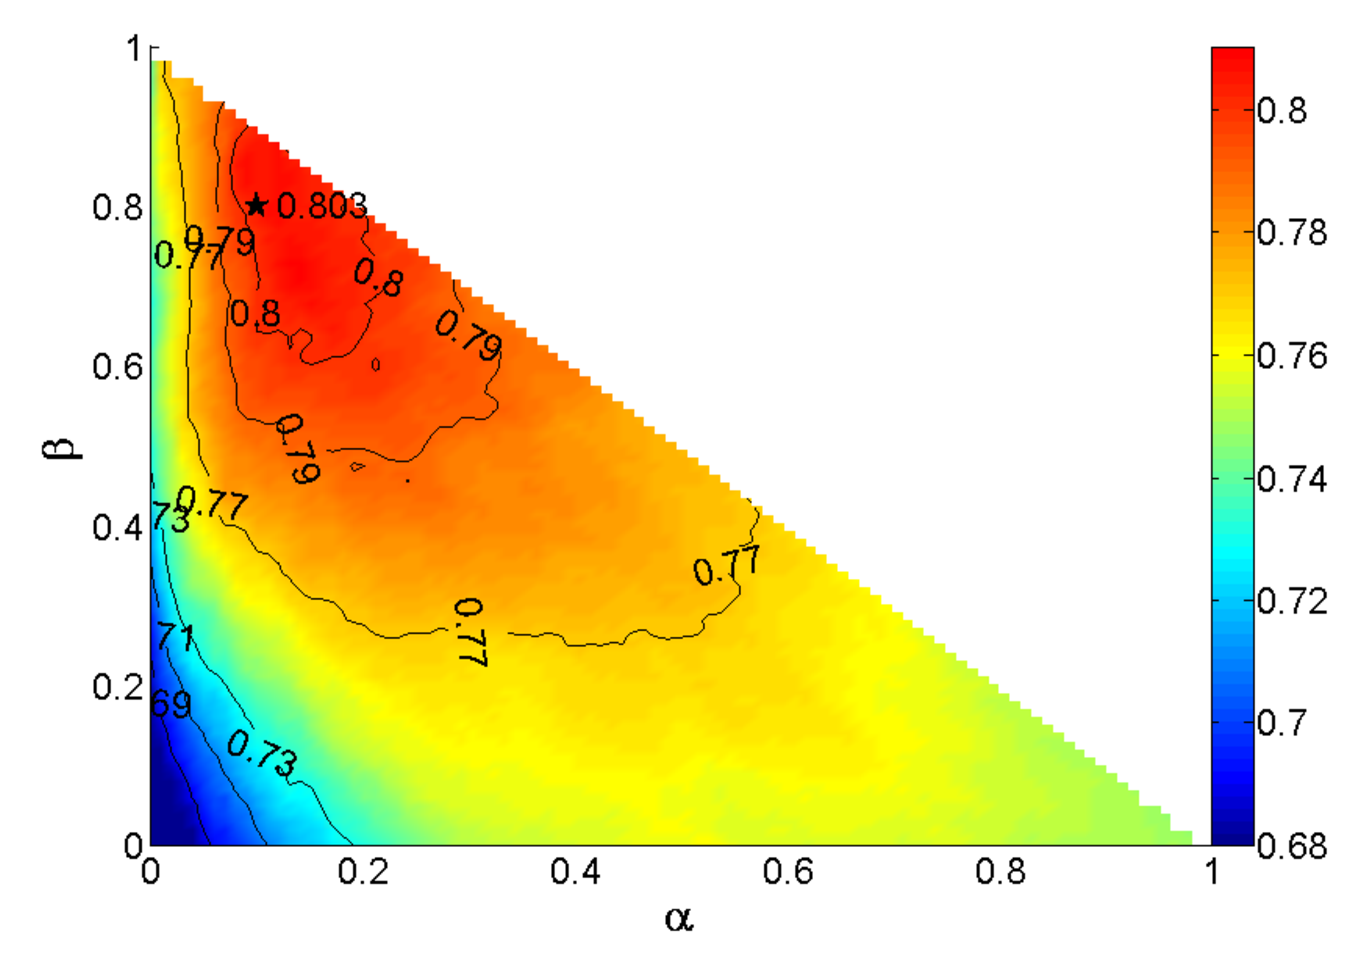
\includegraphics[scale=\graphscaleexpapp]{./exp/AAN-para-recm.eps}}
%\quad\quad
%\hspace{\graphmarginexpapp}
\hfill
\subfigure[{\scriptsize \aminer with \recom}]{\label{exp-aminer-ab-recom}
\includegraphics[scale=\graphscaleexpapp]{./exp/AMiner-para-recm.eps}}
%\quad\quad
%\hspace{\graphmarginexpapp}
\hfill
\subfigure[{\scriptsize \magdata with \recom}]{\label{exp-mag-ab-recom}
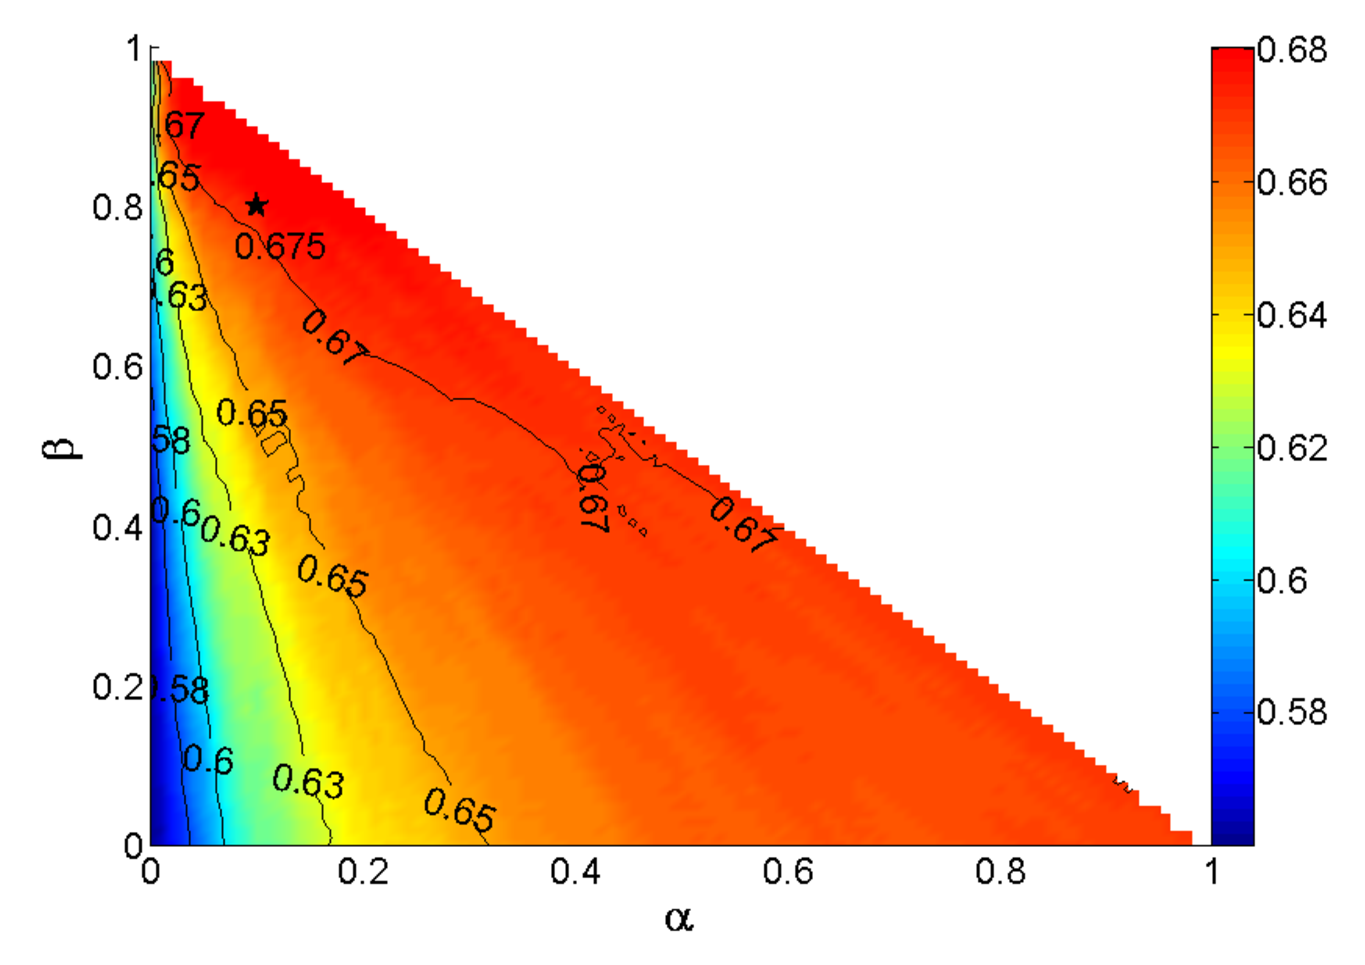
\includegraphics[scale=\graphscaleexpapp]{./exp/MAG-para-recm.eps}}
\\ %%%%%%%%%%%%%%%%%%%%%%%%%%%%%%%%%%%%%%
\vspace{-2ex}
%\hspace{-10ex}
\subfigure[{\scriptsize \aan  with \fcita}]{\label{exp-aan-ab-fcita}
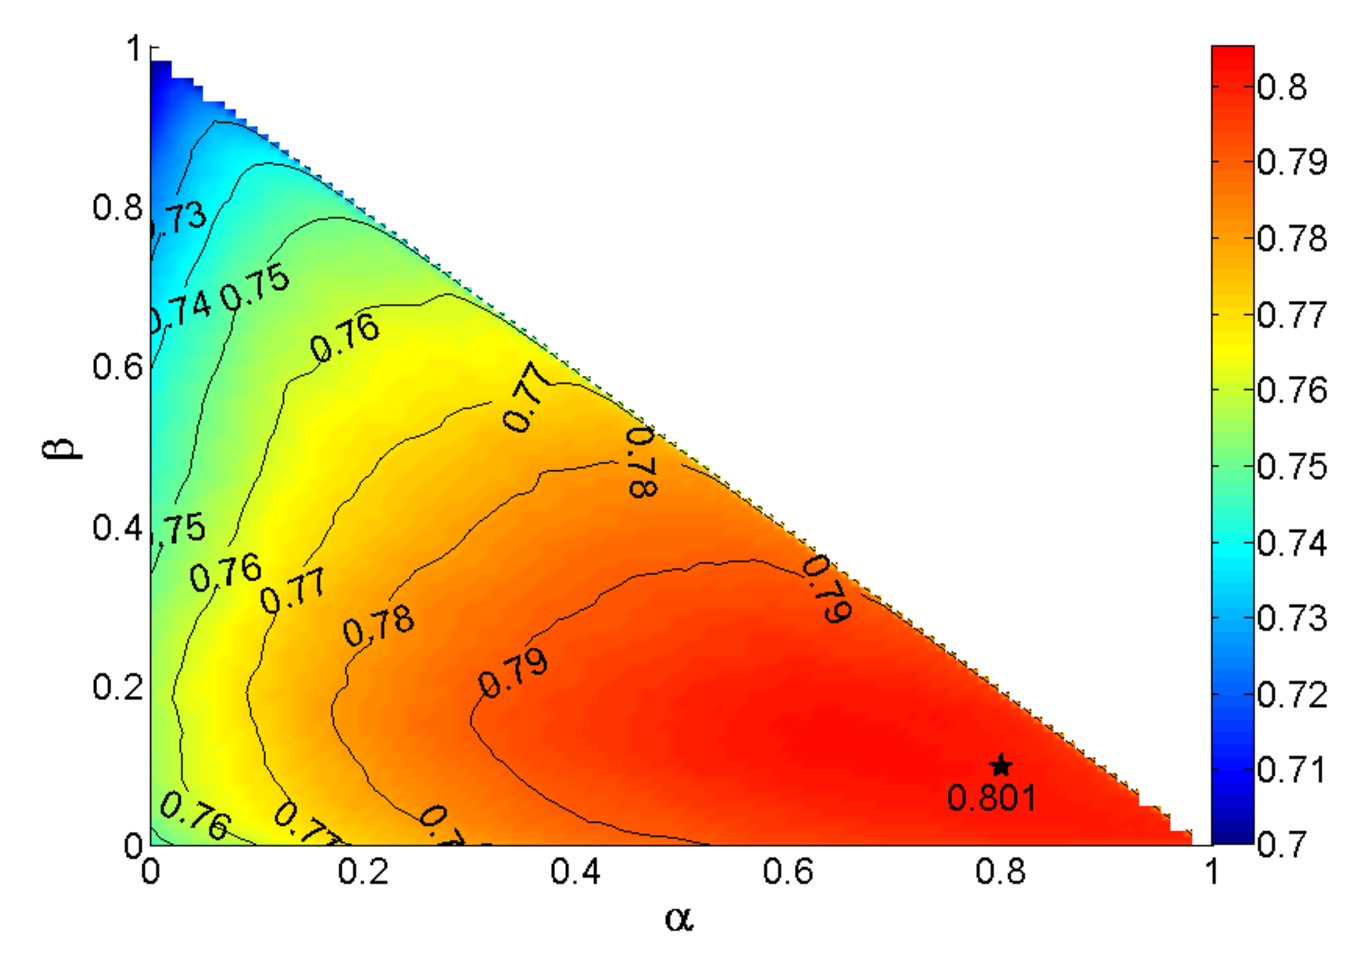
\includegraphics[scale=\graphscaleexpapp]{./exp/AAN-para-fcita.eps}}
%\quad\quad
%\hspace{\graphmarginexpapp}
\hfill
\subfigure[{\scriptsize \aminer with \fcita}]{\label{exp-aminer-ab-fcita}
\includegraphics[scale=\graphscaleexpapp]{./exp/AMiner-para-fcita.eps}}
%\quad\quad
%\hspace{\graphmarginexpapp}
\hfill
\subfigure[{\scriptsize \magdata with \fcita}]{\label{exp-mag-ab-fcita}
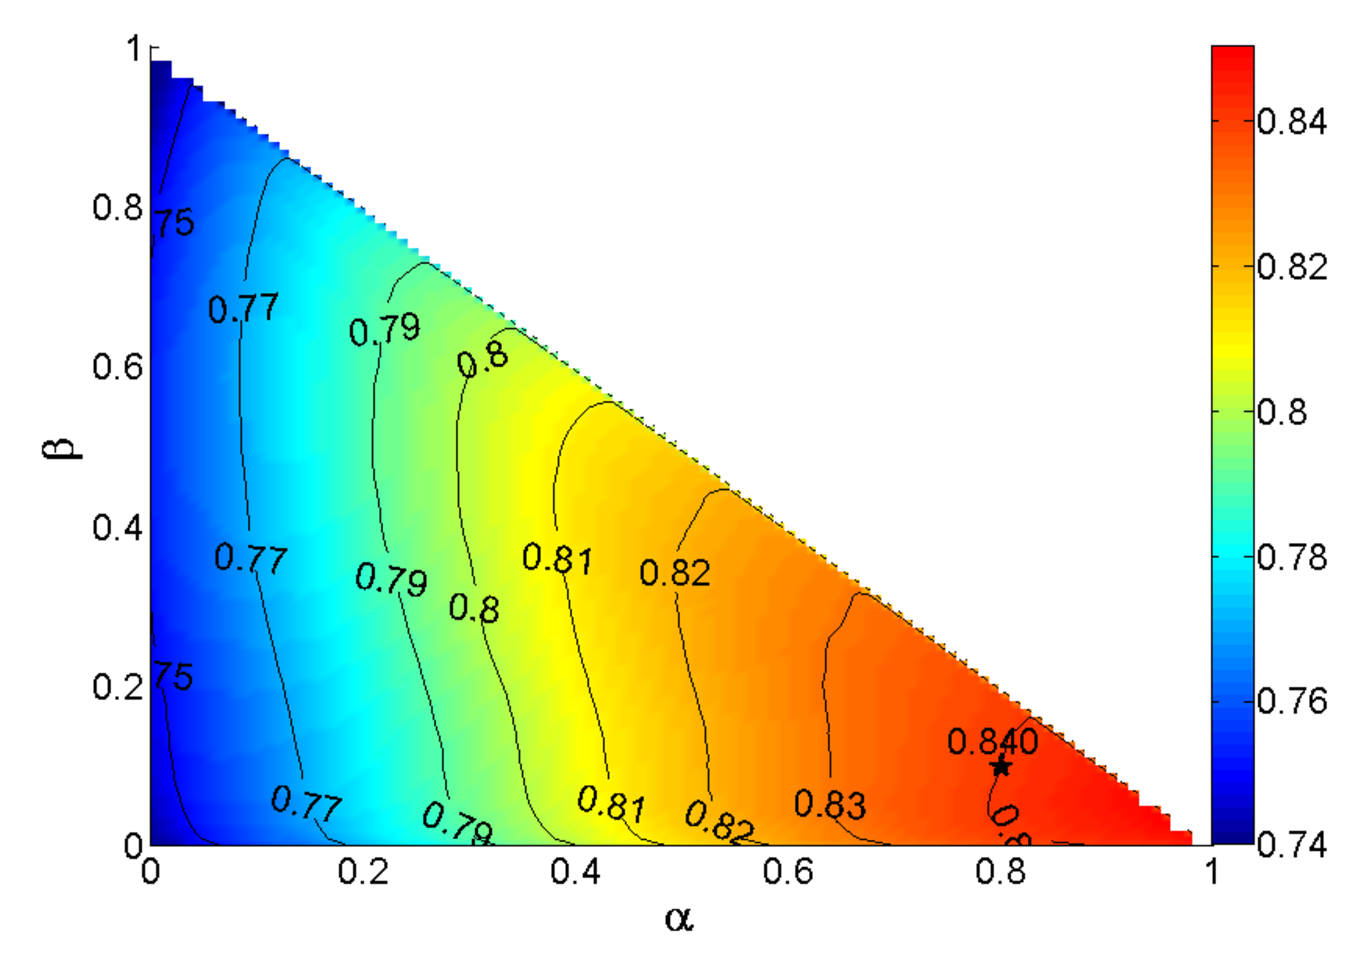
\includegraphics[scale=\graphscaleexpapp]{./exp/MAG-para-fcita.eps}}
\end{center}
\vspace{-2.5ex}
\caption{\small Accuracy tests: varying aggregating parameters $\alpha$ and $\beta$}
\label{exp-ab}
\vspace{-3ex}
\end{figure*}
%%%%%%%%%%%%%%%%%%%%%%%%%%%%%%%%%%%%%%

\stitle{Exp-4: Impacts of parameters}.
%\subsubsection{Exp-4: Impacts of parameters}.
In the last set of tests, we evaluated the impacts of time decaying factor $\sigma$, importance weighting factor $\lambda$, aggregating parameters $\alpha$ and $\beta$, and the TWPageRank. We fixed these parameters as well as $Y_s$ to their default values, used the TWPageRank proposed in this work by default, and tested the \PairAcc with the entire \recom and \fcita (\ie $T_i=+\infty$, $dif=1$).

%We present main results only and more details are available in~\cite{SARank-full}.




\etitle{Exp-4.1}.
%\stitle{Exp-4.1}.
To evaluate the impacts of the time decaying factor $\sigma$, we varied $\sigma$ from -1.6 to -0.4.
%, while fixed $Y_s$ to default values, $T_i=+\infty$, $dif=1$ and $\lambda=0.5$.
The results of \PairAcc are reported in Figs.~\ref{exp-aan-sigma}, \ref{exp-aminer-sigma} and \ref{exp-mag-sigma}.
%with both sets of ground-truth


When varying $\sigma$, the \PairAcc of \ensemblerank is very stable on all datasets using both \recom and \fcita. Indeed, with \recom and \fcita, the \PairAcc only varies (0.42\%, 1.55\%, 0.81\%) and (1.26\%, 0.96\%, 1.16\%) on (\aan, \aminer, \magdata), respectively.
%
%We omitted the detailed results of running time due to space constraint.
The running time varies (11.3\%, 8.6\%) on average only on (\aminer, \magdata), respectively.
%(0.18, 33.6) seconds, \ie

%Both of these show the robustness of \ensemblerank to the time decaying factor $\sigma$.

%As we can see from the figure, our method \ensemblerank is almost stable with the reduction of $\sigma$, since there is only a small fluctuation and the accuracy of our methods is always higher than the best baseline result in all datasets regardless of the change of $\sigma$. This means \ensemblerank is insensitive with $\sigma$.


%%%%%%%%%%%%%%%%%%%%%%%%%%%%%%%%%%%%%%%%%%%%%%%%%%
\begin{table}[tb!]
%\vspace{-2ex}
\begin{center}
\caption{\small Accuracy tests using different components with \recom (rows 2--4) and \fcita (rows 5--7).}
\label{tab-recom}
\begin{small}
\vspace{-.5ex}
\begin{tabular}{|c| c |c | c|}
\hline
{\bf Datasets} & {\bf C}\hspace{5ex}{\bf V}\hspace{5ex}{\bf A} & {\bf CV}\hspace{3ex}{\bf CA}\hspace{3ex}{\bf VA} & {\bf CVA} \\
\hline \hline
% \recom
\aan & 0.752 \ 0.616 \ 0.649 & 0.809 \ 0.764 \ 0.747 & {\bf 0.810} \\
\aminer & 0.735 \  0.581 \  0.640 & 0.784 \ 0.749 \ 0.729 & {\bf 0.785} \\
\magdata & 0.635 \ 0.534 \ 0.553 & 0.697 \ 0.673 \  0.648 & {\bf 0.698} \\ \hline
% \ficta
\aan & 0.785 \ 0.557 \ 0.761 & 0.849 \ 0.866 \ 0.771 & {\bf 0.870} \\
\aminer & 0.713 \  0.603 \  0.725 & 0.843 \ 0.847 \ 0.740 & {\bf 0.856} \\
\magdata & 0.736 \ 0.628 \ 0.718 & 0.848 \ 0.857 \ 0.751 & {\bf 0.874} \\
\hline
\end{tabular}
\end{small}
\end{center}
\vspace{-6ex}
\end{table}
%%%%%%%%%%%%%%%%%%%


\etitle{Exp-4.2}.
%\stitle{Exp-4.2}.
To evaluate the impacts of importance weighting factor $\lambda$, we varied $\lambda$ from 0 to 1.
%while fixed $Y_s$ to default values, $T_i=+\infty$, $dif=1$ and $\sigma=-1.0$.
The results of \PairAcc are reported in Figs.~\ref{exp-aan-lambda}, \ref{exp-aminer-lambda} and \ref{exp-mag-lambda}. Note that parameter $\lambda$ has no impacts on efficiency.
%with both sets of ground-truth

When varying $\lambda$, the \PairAcc of \ensemblerank first increases and then decreases on all datasets with both \fcita and \recom, except on \aminer with \recom.
%\marked{The value of $\lambda$ for \ensemblerank to achieve the best effectiveness is (0.6, 0, 0.2) and (0.6, 0.4, 0.1) on (\aan, \aminer, \magdata) with \recom and \fcita, respectively.}
This result indicates that combining prestige and popularity generally produces more robust results than using either of prestige and popularity.
Indeed, with \recom and \fcita, the \PairAcc of combining prestige and popularity is (10.2\%, 10.7\%, 5.5\%) and (8.0\%, 8.7\%, 9.0\%) higher than using prestige alone, and is (1.2\%, -0.1\%, 1.0\%) and (1.0\%, 1.0\%, 0.3\%) higher than using popularity alone on (\aan, \aminer, \magdata), respectively.


%The selection of $\lambda$ is influenced by ground-truth, such that the best $\lambda$ falls into $[xx,xx]$ and $[yy,yy]$ on \fcita and \recom, respectively. Moreover, equally weighting, \ie $\lambda=0.5$, is a good default setting when no query information is available in advance.
%Indeed, the best obtained \PairAcc using (\fcita, \recom) is only (0.10\%, 0.38\%), (0.04\%, 2.59\%) and (0.06\%, 0.91\%)  higher than the \PairAcc of equally weighting on \aan, \aminer and \magdata, respectively.





\etitle{Exp-4.3}.
To evaluate the impacts of aggregating parameters $\alpha$ and $\beta$, we varied $\alpha$ and $\beta$ at the granularity of 0.01. Again, parameters $\alpha$ and $\beta$ have few impacts on efficiency. The results are reported in Fig.~\ref{exp-ab}, where the parameters selected earlier and their corresponding \PairAcc are marked with $*$.

When varying $\alpha$ and $\beta$, the \PairAcc of \ensemblerank changes gently, as shown in Fig.~\ref{exp-ab}.
The optimal \PairAcc is obtained within a single region, rather than a complex collection of optimal regions.
%
Moreover, the \PairAcc keeps at a high level within a certain ($\alpha$, $\beta$) combination space around the optimal region, as shown in Fig.~\ref{exp-ab}.
%For instance, consider a square of length 0.3, which covers 8.5\% of the parameter combination space. The fraction of parameters such that the \PairAcc is no worse than 1\% of the corresponding \PairAcc with marker $*$ is (73\%, 94\%) on \aan, (96\%, 87\%) on \aminer and (83\%, 95\%) on \magdata, using (\recom, \fcita), respectively.
%
Further, the optimal parameters on the same sets of ground-truth are very similar for (\aan, \aminer and \magdata), indicating that the setting of $\alpha$ and $\beta$ can be easily transferred across different datasets.
To conclude, \ensemblerank is very robust to parameters $\alpha$ and $\beta$, and it is quite flexible for choosing proper values of parameters $\alpha$ and $\beta$.

Moreover, this enables to verify the effectiveness of importance assembling from different components, whose results are reported in Table~IV, in which letters C, V and A stand for citation, venue and author components, respectively.
The ranking based on all components consistently performs the best, using both \recom and \fcita, which justifies the use of importance assembling for ranking scholarly articles.
%which, using \recom and \fcita, improves the \PairAcc over using components (C, V, A, CV, CA, VA) by (5.77\%, 19.4\%, 16.1\%, 0.09\%, 4.59\%, 6.28\%) and (9.54\%, 23.7\%, 5.90\%, 2.50\%, 0.71\%, 4.79\%) on \aan, (6.94\%, 23.7\%, 14.4\%, 0.21\%, 1.56\%, 7.67\%) and (17.68\%, 12.4\%, 9.61\%, 0.33\%, 1.88\%, 6.34\%) on \aminer, and (6.29\%, 16.38\%, 14.45\%, 0.05\%, 2.43\%, 5.02\%) and (11.43\%, 19.2\%, 11.2\%, 1.44\%, 0.77\%, 9.62\%) on \magdata, respectively.


\eat{
\etitle{Exp-4.3}.
%\stitle{Exp-4.3}.
To evaluate the impacts of aggregating parameters $\alpha$ and $\beta$, we varied $\alpha$ and $\beta$ at the granularity of 0.01.
%while fixed $Y_s$ to default values, $T_i=+\infty$, $dif=1$, $\sigma=-1.0$ and $\lambda=0.5$.
Again, parameters $\alpha$ and $\beta$ have few impacts on efficiency. Due to space limitations, we only present the main results and more details are available at~\cite{SARank-full}.

Indeed, \ensemblerank is very robust to parameters $\alpha$ and $\beta$.
(a) When varying $\alpha$ and $\beta$, the \PairAcc of \ensemblerank changes gently. (b) \PairAcc also keeps at a high level within a certain ($\alpha$, $\beta$)  combination space. Finally, (c) the optimal parameters on the same set of ground-truth are very similar for \aan, \aminer and \magdata. That is, it is quite flexible for choosing proper values
of  parameters $\alpha$ and $\beta$.
} %%%%%%%% brief version of Exp-4.3

%%%%%%%%%%%%%%%%%%%%%%%%%%%%%%%%%%%%%%
\begin{figure*}[tb!]
%\vspace{1ex}
\addtolength{\subfigcapskip}{-1ex}
\begin{center}
\subfigure[{\scriptsize \aan with \recom}]{\label{exp-aan-recom-drank}
\includegraphics[scale=0.35]{./exp/AAN_TWPageRank_recom.eps}}
\hfill
%\hspace{\graphmarginexpapp}
\subfigure[{\scriptsize \aminer with \recom}]{\label{exp-aminer-recom-drank}
\includegraphics[scale=0.35]{./exp/AMiner_TWPageRank_recom.eps}}
\hfill
%\hspace{\graphmarginexpapp}
\subfigure[{\scriptsize \magdata with \recom}]{\label{exp-mag-recom-drank}
\includegraphics[scale=0.35]{./exp/MAG_TWPageRank_recom.eps}}
\\%%%%%%%%%%%%%%%%%%%%%%%%%%%%%%%%%%%%%%%%%%%
\vspace{-1.5ex}
\subfigure[{\scriptsize \aan with \fcita}]{\label{exp-aan-fcita-drank}
\includegraphics[scale=0.35]{./exp/AAN_TWPageRank_fcita.eps}}
\hfill
%\hspace{\graphmarginexpapp}
\subfigure[{\scriptsize \aminer with \fcita}]{\label{exp-aminer-fcita-drank}
\includegraphics[scale=0.35]{./exp/AMiner_TWPageRank_fcita.eps}}
\hfill
%\hspace{\graphmarginexpapp}
\subfigure[{\scriptsize \magdata with \fcita}]{\label{exp-mag-fcita-drank}
\includegraphics[scale=0.35]{./exp/MAG_TWPageRank_fcita.eps}}
\end{center}
\vspace{-2.5ex}
\caption{\small Impacts of the TWPageRank on accuracy: varying importance weighting
factor $\lambda$}
\label{exp-drank}
\vspace{-3ex}
\end{figure*}
%%%%%%%%%%%%%%%%%%%%%%%%%%%%%%%%%%

\newcommand{\drank}{\kw{DRank}}


\etitle{Exp-4.4}.
\marked{To evaluate the impacts of the proposed TWPageRank, we compared our approach \ensemblerank with an algorithm alternative (referred to as \drank) the same to \ensemblerank except exploiting exponentially decayed impact weights, \ie $w(u,v)=e^{\sigma(T_u-T_v)}$ in Eq.~(\ref{eq-infl-weights}).
%The two algorithms produce the same popularity while different prestige.
To better understand the impacts, we varied the importance weighting factor $\lambda$ from 0.1 to 1. Note that the ranking results are the same when $\lambda=0$ due to the same popularity computation. The results are reported in Fig.~\ref{exp-drank}, where the numbers represent the improvement of \PairAcc by \ensemblerank over the one by \drank.}

\marked{
When varying $\lambda$, the \PairAcc of \ensemblerank is better than the one of \drank in most cases, which shows the superiority of the TWPageRank than exploiting exponentially decayed weights.
The difference of \PairAcc by the two algorithms is higher with \recom than with \fcita, since the two algorithms are using citation information to predict past and future citations with \fcita.
Moreover, algorithm \ensemblerank is consistently better than \drank when $0.5 \le \lambda \le 0.9$.
%, which, with \recom and \fcita, improves the \PairAcc by (2.88\%, 3.91\%, 3.90\%) and (0.55\%, 0.50\%, 0.22\%) on (\aan, \aminer, \magdata) on average, respectively.
The improvement decreases with the decrease of $\lambda$ as the popularity dominates the ranking with small $\lambda$, and in some cases, \drank outperforms \ensemblerank. %as the prestige and popularity orders of article pairs are more diverse for \drank than \ensemblerank.
Overall, with \recom and \fcita, \ensemblerank improves the \PairAcc over \drank by (1.78\%, 3.07\%, 3.20\%) and (0.29\%, 0.48\%, 0.11\%) on (\aan, \aminer, \magdata) on average, respectively.
}

\marked{
The TWPageRank has little impacts on efficiency, and the running time of the two algorithms only varies (6.34\%, 4.83\%) on (\aminer, \magdata) on average, respectively.}

\eat{
With the increment of $\lambda$, \ensemblerank has more promotion than DRank and the \PairAcc of DRank is better than \ensemblerank with small $\lambda$, possibly due to the addition of popularity will correct the mistaken pairs better on DRank, although \ensemblerank rank more pairs correctly.
In addition, the change of \PairAcc with \recom is higher than the one with \fcita, possibly due to the article pairs in \fcita are of the same years.
Moreover, the \PairAcc of \ensemblerank is better than its counterparts from $\lambda=0.5$ to $\lambda=1$, except on \aminer with \fcita. Recall that in Fig.~\ref{exp-aminer-lambda} using popularity alone gives the best results on \aminer, indicating that the prestige computed by TWPageRank is less accurate on \aminer than on the other two datasets.
%
Indeed, with \recom and \fcita, the \PairAcc of \ensemblerank is (2.20\%, 6.63\%, 5.68\%) and (0.25\%, 0.05\%, 0.05\%) higher than DRank on (\aan, \aminer, \magdata), respectively, when using prestige alone, and is (1.73\%, 2.97\%, 2.92\%) and (0.22\%, -0.08\%, 0.17\%) higher when combining prestige and popularity, respectively, on average.
%
Finally, the TWPageRank has little impacts on efficiency, and the running time of \ensemblerank and its counterparts only changes (6.34\%, 4.83\%) on (\aminer, \magdata) on average, respectively.
}

\stitle{Summary}.
From these tests we find the followings.


\sstab(1) Our model \ensemblerank is effective for ranking scholarly articles, which is consistently better than competitive methods in all tests. With \recom and \fcita, \ensemblerank improves \PairAcc over (\pagerank, \futurerank, \hhgrank) by
(13.5\%, 6.8\%, 4.8\%) and (12.0\%, 3.0\%, 3.2\%) on \aan,
(12.7\%, 5.0\%, 4.9\%) and (14.0\%, 6.5\%, 4.6\%) on \aminer, and
(6.5\%, 2.5\%, 2.2\%) and (13.4\%, 6.0\%, 2.4\%) on \magdata, on average, respectively.
%, and it has a great advantage in evaluating the importance in a long term. Furthermore, it is more accurate evaluating articles which have just published and is in lack of citations, since it uses both venue network and author information besides of citation network. Indeed, it improves the accuracy by $(7.9\%, 3.2\%, 2.3\%)$ and $(14.4\%, 5.0\%, 3.8\%)$ over \pagerank, \futurerank and \hhgrank on average of three datasets with recommendation based ground truth and future citation ground truth, respectively.


\sstab(2) Our batch algorithm \batensemble and incremental algorithm \incensemble are also efficient.
%
Our incremental algorithm \incensemble is on average (1.7, 3.1, 2.8, 117) and (2.0, 3.0, 4.4, 245) times faster than (\batensemble, \powensemble, \futurerank, \hhgrank)  on the large \aminer and \magdata, respectively.

%The batch algorithm \batensemble is on average (1.3, 2.5, 348) times faster than (\powensemble, \futurerank, \hhgrank)  on the largest \magdata, respectively.

%\noindent (3) Our incremental algorithms are much faster than their batch counterparts in practice, even their time complexity is very close. Indeed, algorithms \inctwprdag, \inctwprscc and \incensemble further improve the efficiency of (\twprdag, \twprscc, \batensemble) by (23\%, 38\%, 22\%) on average, respectively.


\sstab(3) Our ranking model \ensemblerank introduces the time decaying factor $\sigma$, importance weighting factor $\lambda$ and aggregating parameters $\alpha$ and $\beta$ for the sake of practicability and flexibility in real-life applications, and, from our tests, \ensemblerank is very robust to these parameters. Moreover, the proposed TWPageRank is generally more effective than directly using exponentially decayed impact weights.




%%%%%%%%%%%%%%%%%%%%%%%%%%%%%%%%%%%%%%%%%%%%%%%%%%%%%%%%%%%%%%%%%%%%%%%%%%%%%%
\section{Experimental Study} %
\label{sec-exp}
%%%%%%%%%%%%%%%%%%%%%%%%%%%%%%%%%%%%%%%%%%%%%%%%%%%%%%%%%%%%%%%%%%%%%%%%%%%%%%


In this section, we present an extensive experimental study of our one-pass trajectory simplification algorithms (\cist and \cista) compared with the \textcolor{blue}{compression} optimal algorithm using \sed (\osed) and existing algorithms of \dps and \squishe on trajectory datasets.
%
Using four real-life trajectory datasets, we conducted sets of experiments to evaluate:
(1) the compression ratios of algorithms \cist and \cista vs. \dps, \squishe and \osed,
(2) the average errors of algorithms \cist and \cista vs. \dps, \squishe and \osed,
(3) the running time of algorithms \cist and \cista vs. \dps, \squishe and \osed,
(4) the impacts of polygon intersection algorithms \rpia and \cpia and the edge number $m$ of inscribed regular polygons to the compression ratios, errors and running time of algorithms \cist and \cista,
(5) the impacts of the distance metrics \ped and \sed on the compression ratios, errors and running time of trajectory simplification algorithms, and
{(6) the impacts of the distance metrics \ped and \sed on spatio-temporal queries.}


\subsection{Experimental Setting}
%We first introduce the settings of our experimental study.

\stitle{Real-life Trajectory Datasets}.
We use four real-life datasets \sercar, \geolife, \mopsi and \pricar shown in Table~\ref{tab:datasets} to test our solutions.

% \ni \emph{(1) Truck trajectory data} (\truck) is the GPS trajectories collected by \eat{10,368} trucks equipped with GPS sensors in China
% during a period from Mar. 2015 to Oct. 2015. The sampling rate varied from 1s to 60s.
%Trajectories mostly have around $50$ to $90$ thousand data points.

\vspace{0.5ex}
\ni \emph{(1) Service car trajectory data} (\sercar) is the GPS trajectories collected by a Chinese car rental company during Apr. 2015 to Nov. 2015. The sampling rate was one point per $3$--$5$ seconds, and
each trajectory has around $114.1K$ points.
%.We randomly chose $1,000$ cars from them

\vspace{0.5ex}
\ni \emph{(2) GeoLife trajectory data} (\geolife) is the GPS trajectories collected in GeoLife project~\cite{Zheng:GeoLife} by 182 users in a period from Apr. 2007 to Oct. 2011. These trajectories have a variety of sampling rates, among which 91\% are logged with one point per 1-5 seconds. %or each 5-10 meters
%The longest trajectory has 2,156,994 points.

\vspace{0.5ex}
\ni \emph{(3) Mopsi trajectory data} (\mopsi) is the GPS trajectories collected in Mopsi project~\cite{Mopsi} by 51 users in a period from 2008 to 2014. Most routes are in Joensuu region, Finland.
The sampling rate was one point per $2$ seconds, and each trajectory has around $153.9K$ points.
%exist on every continent.

\vspace{0.5ex}
\ni \emph{(4) Private car trajectory data} (\pricar) is a small set GPS trajectories collected with a high sampling rate of one point per second by our team members in 2017. There are 10 trajectories and each trajectory has around 11.8K points.

%{This dataset contains 182 trajectories, one trajectory for each user, with a total distance of about 1.2 million kilometers. }

\vspace{0.5ex}
As the \textcolor{blue}{compression} optimal algorithm \osed \cite{Imai:Optimal} has both high time and space complexities, \ie $O(n^3)$ time and $O(n^2)$ space, it is impossible to compress the entire datasets (slow and out of memory). Hence, we further build four \textit{small datasets} such that each includes 10 middle-size ($10K$ points per trajectory) trajectories selected from \sercar, \geolife, \mopsi and \pricar, respectively.

%The details of these datasets are shown in Table~\ref{tab:dataset}.

\stitle{Algorithms and implementation}.
We implement seven \lsa algorithms, \ie our \cist and \cista,  sector intersection algorithm using \ped (\kw{SIPED})~\cite{Dunham:Cone, Zhao:Sleeve}, \kw{DPPED} and \dps (\dpa using \ped~\cite{Douglas:Peucker} and \dpa using \sed~\cite{Meratnia:Spatiotemporal}, the existing sub-optimal \lsa algorithms having the best compression ratios), \squishe~\cite{Muckell:Compression} (the fastest existing \lsa algorithm using \sed) and \osed~\textcolor{blue}{(the compression optimal \lsa algorithm using \sed, see Section~\ref{subsec-optimal})}.
We also implement the polygon intersection algorithms, \cpia and our \rpia.

All algorithms were implemented with Java.
All tests were run on an {x64-based  PC with 8 Intel(R) Core(TM) i7-6700 CPU @ 3.40GHz and 8GB of memory, and each test was repeated
over 3 times and the average is reported here.

%
%\textcolor{blue}{
%In the comparation of compression ratio and average error, we selected a subset from the datasets subject to the limit of memory space and time. Concretely, we selected ($100$, $95$, $1000$, $10$) trajectories from datasets {\sercar, \geolife, \mopsi, \pricar} respectively.
%}
%\textcolor{blue}{
%As for efficiency, we use the full dataset, and exclude the optimal algorithm.
%}

%%%%%%%%%%%%%%%%%%%%%%%%%%%%%%%%%%%%%%%%%%%%%%%%%%%%%%%%%%%%%%%%%%%%%%%%%%%%%%
\subsection{Experimental Results}
%%%%%%%%%%%%%%%%%%%%%%%%%%%%%%%%%%%%%%%%%%%%%%%%%%%%%%%%%%%%%%%%%%%%%%%%%%%%%%

We next present our findings.

%%%%%%%%%%%%%%%%%%%%%%%%%%%%%%%%%%%%%%%%%%%%%%%%%%%%%%%%%%%%%%%%%%%%%%%%%%%%%%
\subsubsection{Evaluation of Compression Ratios}
%%%%%%%%%%%%%%%%%%%%%%%%%%%%%%%%%%%%%%%%%%%%%%%%%%%%%%%%%%%%%%%%%%%%%%%%%%%%%%


In the first set of tests, we evaluate the impacts of parameter $m$ on the
compression ratios of our algorithms \cist and \cista, and compare the compression ratios of \cist and \cista with \dps, \squishe and \osed.
%
The compression ratio is defined as follows: Given a set of trajectories $\{\dddot{\mathcal{T}_1}, \ldots, \dddot{\mathcal{T}_M}\}$ and their piece-wise line representations $\{\overline{\mathcal{T}_1}, \ldots, \overline{\mathcal{T}_M}\}$, the compression ratio of an algorithm is $(\sum_{j=1}^{M} |\overline{\mathcal{T}}_j |)/(\sum_{j=1}^{M} |\dddot{\mathcal{T}}_j |)$.
By the definition, \emph{algorithms with lower compression ratios are better}.





%%%%%%%%%%%%%%%%%%%%%%%%%%%%%%%%%%%%%%%%%%%%%%%%%%%%%%%%%%%%%%%%%%%%%%%%%%%%%%%%%%%%%%%%%%%%%
%%%%%%%%%%%%%%%%%%%%%%%%%%%%Compression Ratios


\begin{figure*}[tb!]
\centering
\includegraphics[scale = 0.290]{./Exp-M-e-60-CR-service.png}\hspace{1ex}
\includegraphics[scale = 0.290]{./Exp-M-e-60-CR-geolife.png}\hspace{1ex}
\includegraphics[scale = 0.290]{./Exp-M-e-60-CR-mopsi.png}\hspace{1ex}
\includegraphics[scale = 0.290]{./Exp-M-e-60-CR-private.png}
%\vspace{-1ex}
\caption{\small Evaluation of compression ratios: fixed error bound with $\epsilon=60$ meters and varying $m$.
Here ``R'' denotes our fast regular polygon intersection algorithm \rpia, and ``C'' denotes the convex polygon intersection algorithm \cpia, respectively.}
\label{fig:m-cr-e60}
%\vspace{-1ex}
\end{figure*}


\begin{figure*}[tb!]
\centering
\includegraphics[scale = 0.290]{./Exp-CR-epsilon-service.png}\hspace{1ex}
\includegraphics[scale = 0.290]{./Exp-CR-epsilon-geolife.png}\hspace{1ex}
\includegraphics[scale = 0.290]{./Exp-CR-epsilon-mopsi.png}\hspace{1ex}
\includegraphics[scale = 0.290]{./Exp-CR-epsilon-private.png}
%\vspace{-1ex}
\caption{\small Evaluation of compression ratios: fixed with $m=16$ and varying error bound $\epsilon$.}
\label{fig:cr-m16}
%\vspace{-1.0ex}
\end{figure*}



\begin{figure*}[tb!]
\centering
\includegraphics[scale = 0.290]{./Exp-opt-CR-epsilon-service.png}\hspace{1ex}
\includegraphics[scale = 0.290]{./Exp-opt-CR-epsilon-geolife.png}\hspace{1ex}
\includegraphics[scale = 0.290]{./Exp-opt-CR-epsilon-mopsi.png}\hspace{1ex}
\includegraphics[scale = 0.290]{./Exp-opt-CR-epsilon-private.png}
%\vspace{-1ex}
\caption{\small Evaluation of compression ratios: fixed with $m=16$ and varying error bound $\epsilon$ (on small datasets).}
\label{fig:cr-optimal-m16}
%\vspace{-1.0ex}
\end{figure*}



\begin{figure*}[tb!]
\centering
\includegraphics[scale = 0.2900]{./Exp-CR-size-service.png}\hspace{1ex}
\includegraphics[scale = 0.2900]{./Exp-CR-size-geolife.png}\hspace{1ex}
\includegraphics[scale = 0.2900]{./Exp-CR-size-mopsi.png}\hspace{1ex}
\includegraphics[scale = 0.2900]{./Exp-CR-size-private.png}
%\vspace{-1ex}
\caption{\small Evaluation of compression ratios: fixed with $m=16$ and $\epsilon=60$ meters, and varying the size of trajectories.}
\label{fig:cr-size}
\vspace{-1ex}
\end{figure*}




%\vspace{0.5ex}
\stitle{Exp-1.1: Impacts of parameter $m$ on compression ratios}.
To evaluate the impacts of the number $m$ of edges of polygons on the compression ratios of algorithms \cist and \cista, and also to confirm that our fast regular polygon intersection algorithm \rpia has the same compression ratios as the convex polygon intersection algorithm \cpia,
we fixed the error bound {$\epsilon =60$ meters}, and varied $m$ from $4$ to $40$. The results are reported in Figure~\ref{fig:m-cr-e60}.

\ni(1) Algorithms \cist and \cista using \rpia have the same compression ratios as their counterparts using \cpia for all cases.

\ni(2) When varying $m$, the compression ratios of algorithms
{\cist and \cista} decrease with the increase of $m$ on all datasets.
{The increase of edge number $m$ of a regular polygon makes the  polygon better approximate its corresponding circle, which leads to a higher potential to have common intersections, and has a better compression ratio.}

%The feature is holding on all error bounds $\epsilon$.
%small error bounds, \eg $\epsilon < 60$ meters, and large error bounds, \eg $\epsilon > 60$ meters.

\ni(3) When varying $m$, the compression ratios of algorithms {\cist and \cista} decrease (a) fast when $m < 12$, (b) slowly when $m \in [12, 20]$, and (c) very slowly when $m > 20$. Hence, \emph{the region of $[12, 20]$ is a good candidate region for $m$ in terms of compression ratios.}
Here the compression ratio of $m$=$12$ is only on average {$100.95\%$} of $m$=$20$.


%\ni(1) The polygon intersection algorithms \rpia and \cpia have the same impacts on compression ratios on all datasets. \eg the compression ratio of \rpia equipped simplification algorithm \cist, \ie \cist-\rpia, is the same as the \cpia equipped simplification algorithm, \ie \cist-\cpia, for each $m$.


%\vspace{0.5ex}
\stitle{Exp-1.2: Impacts of the error bound $\epsilon$ on compression ratios (vs. algorithms \dps and \squishe)}.
To evaluate the impacts of error bound $\epsilon$ on compression ratios, we fixed {$m$=$16$}, the middle of $[12, 20]$, and varied $\epsilon$ from $10$ meters to $200$ meters on the entire four datasets, respectively.
The results are reported in Figure~\ref{fig:cr-m16} .
%Figure~\ref{fig:cr-m10}.  and


\ni (1) When increasing $\epsilon$, the compression ratios of all these algorithms decrease on all datasets,
{as it is clear that a larger $\epsilon$ makes more points represented by a line segment, and brings a better compression ratio.}
%\textcolor{blue}{More specifically, the compression ratio $cr$ of each algorithm has approximately an exponential relation to $\epsilon$, \ie $cr=a^\epsilon$, where $a$ is in $(0,1)$.}

\ni (2) Dataset \pricar has the lowest compression ratios, compared with datasets \mopsi, \sercar and \geolife, due to its highest sampling rate,
\sercar has the highest compression ratios due to its lowest sampling rate, and \geolife and \mopsi have the compression ratios in the middle accordingly.

\ni {(3)} Algorithm \cist is better than \squishe ~{and close to} \dps on all datasets and for all $\epsilon$.
%
The compression ratios of \cist are on average {($79.3\%$, $71.9\%$, $67.3\%$, $72.7\%$) and ($109.2\%$, $108.0\%$, $111.7\%$, $109.1\%$)} of \squishe and
\dps on {datasets (\sercar, \geolife, \mopsi, \pricar)}, respectively.
For example, when $\epsilon$ = $40$ meters, the compression ratios of algorithms
\squishe, \cist and \dps are
{($20.0\%$, $8.0\%$, $5.7\%$, $4.9\%$), ($16.1\%$, $5.8\%$, $3.9\%$, $3.6\%$) and ($14.8\%$, $5.4\%$, $3.4\%$, $3.4\%$)} on  {datasets (\sercar, \geolife, \mopsi, \pricar)}, respectively.
{\cist shows better compression ratios than \squishe because \cist applies an approximate policy that includes as many points as possible into a line segment during the process, while \squishe applies a loose error prediction policy, which may ignore too many potential points that could be represented by a line segment  in order to assure the error bound.}

%\textcolor{blue}{\cist shows better compression ratios than \squishe because \cist applies a greedy policy, \ie it includes as many points as possible into a line segment, while \squishe applies a loose distancce checking policy, \ie it estimates the lowest \sed error and removes the point ``predicted to introduce the lowest amount of error into the compression\cite{Muckell:Compression}" . Its prediction method is not accurate enough, thus, in order to ensure the error bound, it may ignore too many potential points that could be represented by a line segment.}

\ni {(4)} Algorithm \cista has better compression ratios than \dps, \squishe and \cist on all datasets and for all $\epsilon$.
The compression ratios of \cista are on average ($57.7\%$, $53.8\%$, $50.0\%$, $54.6\%$), ($79.5\%$, $81.0\%$, $83.0\%$, $82.0\%$) and {($72.9\%$, $75.0\%$, $74.3\%$, $75.1\%$) of algorithms
\squishe, \dps and \cist on {datasets (\sercar, \geolife, \mopsi, \pricar)}, respectively.
For example, when $\epsilon$ = $40$ meters, the compression ratios of algorithm
\cista are ($11.5\%$, $4.3\%$, $2.8\%$, $2.7\%$) on datasets (\sercar, \geolife, \mopsi, \pricar), respectively.
%
{Algorithm CISED-W extends the radii of base circles of spatio-temporal cones from $\epsilon/2$ in CISED-S to $\epsilon$, thus, it has better compression ratios than \cist.}

%\vspace{0.5ex}
\stitle{Exp-1.3: Impacts of the error bound $\epsilon$ on compression ratios (vs. the \textcolor{blue}{compression} optimal algorithm).}
To evaluate the impacts of error bound $\epsilon$ on compression ratios, we again fixed {$m$=$16$}, the middle of $[12, 20]$, and varied $\epsilon$ from $10$ to $200$ meters on the first $1K$ points of each trajectory of the selected \textit{small datasets}, respectively.
The results are reported in Figure~\ref{fig:cr-optimal-m16} .
%Figure~\ref{fig:cr-m10}.  and

\ni {(1)} Algorithm \cist is worse than the \textcolor{blue}{compression} optimal algorithm \osed~on all datasets and for all $\epsilon$.
More specifically, the compression ratios of \cist are on average ($134.6\%$, $150.7\%$, $155.5\%$, $138.5\%$) of \osed~on {datasets (\sercar, \geolife, \mopsi, \pricar)}, respectively.
For example, when $\epsilon$ = $40$ meters, the compression ratios of \cist and \osed~are
($22.0\%$, $5.9\%$, $1.9\%$, $3.3\%$) and {($16.4\%$, $4.2\%$, $0.9\%$, $2.4\%$)}
on  {datasets (\sercar, \geolife, \mopsi, \pricar)}, respectively.

\ni {(2)} Algorithm \cista~has the closest compression ratios to the \textcolor{blue}{compression} optimal algorithm \osed~on all datasets and for all $\epsilon$.
The compression ratios of \cista are on average  ($94.8\%$, $115.5\%$, $119.7\%$, $107.5\%$)} of \osed~on {datasets (\sercar, \geolife, \mopsi, \pricar)}, respectively.
For example, when $\epsilon$ = $40$ meters, the compression ratios of algorithm
\cista are ($14.6\%$, $4.6\%$, $1.2\%$, $2.5\%$) on datasets (\sercar, \geolife, \mopsi, \pricar), respectively.
%
{ This is because algorithm CISED-W allows data interpolations, by Proposition \ref{prop-circle-intersection}, it extends the radii of the base circles of the spatio-temporal cones from $\epsilon/2$ in CISED-S to $\epsilon$ in CISED-W to contain more points.}

\stitle{Exp-1.4: Impacts of trajectory sizes on compression ratios}.
To evaluate the impacts of trajectory size, \ie the number of data points in a trajectory, on compression ratios,
we chose the same {$10$} trajectories from datasets \sercar, \geolife, \mopsi and \pricar, respectively,
fixed {$m$=$16$} and $\epsilon$=$60$ meters, and varied the size \trajec{|T|} of trajectories from $1K$ points to $10K$ points.
%
The results are reported in Figure~\ref{fig:cr-size}.

\ni(1) The compression ratios of these algorithms ordered from the best to the worst are \cista, \dps, \cist and \squishe, on all datasets with all sizes of trajectories, {which is consistent with the previous tests}.

\ni(2) The sizes of input trajectories have few impacts on the compression ratios of \lsa algorithms on all datasets.





%%%%%%%%%%%%%%%%%%%%%%%%%%%%%%%%%%%%%%%%%%%%%%%%%%%%%%%%%%%%%%%%%%%%%%%%%%%%%%
\subsubsection{Evaluation of Average Errors}
%%%%%%%%%%%%%%%%%%%%%%%%%%%%%%%%%%%%%%%%%%%%%%%%%%%%%%%%%%%%%%%%%%%%%%%%%%%%%%

%%%%%%%%%%%%%%%%%%%%%%%%%%%%%%%%%%%%%%%%%%%%%%%%%%%%%%%%%%%%%%%%%%%%%%%%%%%%
%Average error
%%%%%%%%%%%%%%%%%%%%%%%%%%%%%%%%%%%%%%%%%%%%%%%%%%%%%%%%%%%%%%%%%%%%%%%%%%%%


\begin{figure*}[tb!]
	\centering
	\includegraphics[scale = 0.2900]{./Exp-M-e-60-error-service.png}\hspace{1ex}
	\includegraphics[scale = 0.2900]{./Exp-M-e-60-error-geolife.png}\hspace{1ex}
	\includegraphics[scale = 0.2900]{./Exp-M-e-60-error-mopsi.png}\hspace{1ex}
	\includegraphics[scale = 0.2900]{./Exp-M-e-60-error-private.png}
	%\vspace{-1ex}
	\caption{\small Evaluation of average errors: fixed error bound with $\epsilon = 60$ meters and varying $m$.
Here ``R'' denotes our fast regular polygon intersection algorithm \rpia, and ``C'' denotes \cpia, respectively.}
	\label{fig:m-error-e60}
	%\vspace{-1ex}
\end{figure*}


\begin{figure*}[tb]
	\centering
	\includegraphics[scale = 0.2900]{./Exp-error-epsilon-service.png}\hspace{1ex}
	\includegraphics[scale = 0.2900]{./Exp-error-epsilon-geolife.png}\hspace{1ex}
	\includegraphics[scale = 0.2900]{./Exp-error-epsilon-mopsi.png}\hspace{1ex}
	\includegraphics[scale = 0.2900]{./Exp-error-epsilon-private.png}
	%\vspace{-1ex}
	\caption{\small Evaluation of average errors: fixed with $m=16$ and varying error bound $\epsilon$.}
	\label{fig:ae-m16}
	%\vspace{-1ex}
\end{figure*}





\begin{figure*}[tb]
	\centering
	\includegraphics[scale = 0.2900]{./Exp-opt-error-epsilon-service.png}\hspace{1ex}
	\includegraphics[scale = 0.2900]{./Exp-opt-error-epsilon-geolife.png}\hspace{1ex}
	\includegraphics[scale = 0.2900]{./Exp-opt-error-epsilon-mopsi.png}\hspace{1ex}
	\includegraphics[scale = 0.2900]{./Exp-opt-error-epsilon-private.png}
	%\vspace{-1ex}
	\caption{\small Evaluation of average errors: fixed with $m=16$ and varying error bound $\epsilon$ (on small datasets).}
	\label{fig:ae-optimal-m16}
	%\vspace{-1ex}
\end{figure*}




\begin{figure*}[tb!]
	\centering
	\includegraphics[scale = 0.2900]{./Exp-error-size-service.png}\hspace{1ex}
	\includegraphics[scale = 0.2900]{./Exp-error-size-geolife.png}\hspace{1ex}
	\includegraphics[scale = 0.2900]{./Exp-error-size-mopsi.png}\hspace{1ex}
	\includegraphics[scale = 0.2900]{./Exp-error-size-private.png}
	%\vspace{-1ex}
	\caption{\small Evaluation of average errors: fixed with $m=16$ and $\epsilon=60$ meters, and varying the size of trajectories.}
	\label{fig:ae-size}
	%\vspace{-1ex}
\end{figure*}


In the second set of tests, we first evaluate the impacts of parameter $m$ on the average errors of algorithms \cist and \cista, then compare the average errors of our algorithms \cist and \cista with \dps, \squishe and the \textcolor{blue}{compression} optimal algorithm \osed.

Given a set of trajectories $\{\dddot{\mathcal{T}_1}, \ldots, \dddot{\mathcal{T}}_M\}$ and their piecewise line representations $\{\overline{\mathcal{T}_1}, \ldots, \overline{\mathcal{T}}_M\}$, and point $P_{j,i}$ denoting
a point in trajectory $\dddot{\mathcal{T}}_j$ contained in a line segment $\mathcal{L}_{l,i}\in\overline{\mathcal{T}_l}$ ($l\in[1,M]$),
then the average error is $\sum_{j=1}^{M}\sum_{i=0}^{M} d(P_{j,i},
\mathcal{L}_{l,i})/\sum_{j=1}^{M}{|\dddot{\mathcal{T}}_j |}$.




%%%%%%%%%%%%%%%%%%%%%%%%%%%%%%%%%%%%%%%%%%%%%%%%%%%%%%%%%%%%%%%%%%%%%%%%%
%\vspace{0.5ex}
\stitle{Exp-2.1: Impacts of parameter $m$ on average errors}.
To evaluate the impacts of parameter $m$ on average errors of algorithms \cist and \cista, and to confirm that our fast regular polygon intersection algorithm \rpia has the same average errors as the convex polygon intersection algorithm \cpia,
we fixed the error bound {$\epsilon =60$ meters}, and varied $m$ from $4$ to $40$. The results are reported in Figure~\ref{fig:m-error-e60}.


%\ni(1) The polygon intersection algorithms \rpia and \cpia have the same impacts on average errors on all datasets. \eg the average error of \rpia equipped simplification algorithm \cist, \ie \cist-\rpia, is the same as the \cpia equipped algorithm, \ie \cist-\cpia, for each $m$.

\ni(1) Algorithms \cist and \cista using \rpia have the same average errors as their counterparts using \cpia, respectively, on all datasets and for all $m$.

\ni(2) When varying $m$, the average errors of algorithms \cist and \cista increase with the increase of $m$ on all datasets.
{The increase of edge number $m$ of a regular polygon makes the polygon more closely approximate its corresponding circle, which means that some points having larger \sed, \ie closer to half-$\epsilon$ in \cist or $\epsilon$ in \cista, are also included to a line segment, which further leads to a larger average error.}

\ni(3) When varying $m$, similar to compression ratios, the average errors of
algorithms \cist and \cista increase (a) fast when $m < 12$, (b) slowly when $m
\in [12, 20]$, and (c) very slowly when $m > 20$.
\emph{The range of $[12, 20]$ is also the good candidate region for $m$ in terms of errors.}
Here the average error of $m=12$ is only on average {$98.49\%$} of $m=20$.




%%%%%%%%%%%%%%%%%%%%%%%%%%%%%%%%%%%%%%%%%%%%%%%%%%%%%%%%%%%%%%%%%%%%%%%%%
%\vspace{0.5ex}
\stitle{Exp-2.2: Impacts of the error bound $\epsilon$ on average errors (vs. algorithms \dps and \squishe)}.
To evaluate the average errors of these algorithms, we fixed {$m$=$16$}, and
varied $\epsilon$ from $10$ to $200$ meters on the entire
{datasets} \sercar, \geolife, \mopsi and \pricar, respectively.
The results are reported in Figure~\ref{fig:ae-m16}.

\ni(1) Average errors increase with the increase of $\epsilon$.
{More specifically, the average error of each algorithm has approximately a linear relation to $\epsilon$.}
{It is clear that a larger $\epsilon$ includes more points into a line segment, including points with larger \sed, which brings a better compression ratio as well as a larger average error.}

\ni(2) The average errors of these algorithms from the largest to the smallest are \cista, \cist, \dps and \squishe, on all datasets and for all $\epsilon$.
The average errors of algorithms \cist and \cista are on average
($119.3\%$, $127.7\%$, $119.9\%$, $138.0\%$)
and ($210.1\%$, $207.5\%$, $200.9\%$, $217.5\%$)
of \dps and ($188.2\%$, $215.2\%$, $212.8\%$, $180.3\%$) and
($331.1\%$, $349.7\%$, $356.7\%$, $284.2\%$)
 of \squishe on datasets (\sercar, \geolife, \mopsi, \pricar), respectively.
{Algorithms \cista and \cist apply an approximate policy, \ie they include as many points as possible into a line segment, and this policy usually leads to a larger average error.}

\ni(3) When the error bound of algorithm \cista is set as the half of \cist, the
average errors of \cista are on average ($93.8\%$, $86.0\%$, $81.4\%$, {$79.4\%$}) of \cist on {datasets} (\sercar, \geolife,\mopsi, \pricar), respectively, meaning that the large average errors of algorithm \cista are caused by its cone \wrt $\epsilon$ compared with the narrow cone \wrt $\epsilon/2$ of \cist.
%\ni(2) All datasets have the similar average error in every $\epsilon$.
%\ni(3) Algorithm \squishe has lower average errors than algorithms \dps and \cist on all datasets and all $\epsilon$ values.

%%%%%%%%%%%%%%%%%%%%%%%%%%%%%%%%%%%%%%%%%%%%%%%%%%%%%%%%%%%%%%%%%%%%%%%%%
%\vspace{0.5ex}
\stitle{Exp-2.3: Impacts of the error bound $\epsilon$ on average errors (vs. the \textcolor{blue}{compression} optimal algorithm).}
To evaluate the average errors of these algorithms, we fixed {$m$=$16$}, and
varied $\epsilon$ from $10$ to $200$ meters on the first $1K$ points of each trajectory of the \textit{small datasets}, respectively.
The results are reported in Figure~\ref{fig:ae-optimal-m16}.

The average errors of these algorithms from the largest to the smallest are \cista, the \textcolor{blue}{compression} optimal algorithm \osed~and \cist, on all datasets and for all $\epsilon$.
The average errors of \cist and \cista are on average
($73.6\%$, $80.7\%$, $85.1\%$, $81.0\%$)
and ($133.3\%$, $130.7\%$, $131.0\%$, $126.3\%$)
of \osed~on datasets (\sercar, \geolife, \mopsi, \pricar), respectively.
\textcolor{blue}{Note that here algorithm \osed~has the worst average error among all strong line simplification algorithms, as algorithm \osed~is optimal in terms of compression ratio, and algorithms with better compression ratios generate less line segments, which usually leads to larger errors.}

%%%%%%%%%%%%%%%%%%%%%%%%%%%%%%%%%%%%%%%%%%%%%%%%%%%%%%%%%%%%%%
%\vspace{0.5ex}
\stitle{Exp-2.4: Impacts of trajectory sizes on average errors}.
To evaluate the impacts of trajectory sizes on average errors, we chose the same
{$10$} trajectories from  datasets \sercar, \geolife, \mopsi and \pricar, respectively.
We fixed {$m$=$16$} and $\epsilon = 60$ meters, and varied the size \trajec{|T|} of trajectories from $1K$ points to $10K$ points.
%
The results are reported in Figure~\ref{fig:ae-size}.

\ni(1) The average errors of these algorithms ordered from the smallest to the largest are \squishe, \dps, \cist and \cista, on all datasets and for all trajectory sizes, which is consistent with the above tests.
 %, which is consistent with Figure~\ref{fig:ae-m16}.

\ni(2) The sizes of input trajectories have few impacts on the average errors of \lsa algorithms on all datasets.



	





%%%%%%%%%%%%%%%%%%%%%%%%%%%%%%%%%%%%%%%%%%%%%%%%%%%%%%%%%%%%%%%%%%%%%%%%%%%%%%
\subsubsection{Evaluation of Running Time}
%%%%%%%%%%%%%%%%%%%%%%%%%%%%%%%%%%%%%%%%%%%%%%%%%%%%%%%%%%%%%%%%%%%%%%%%%%%%%%

In the third set of tests, we evaluate the impacts of parameter $m$ on the running time of algorithms \cist and \cista, and compare the running time of our approaches \cist and \cista with algorithms \osed, \dps and \squishe.

%\ie the edge number of a regular polygon,
%
%The execution time is the running time of the compressing process.
%For a small size trajectory, we repeat compress it tens of times and accumulation the total running time so as to get the average compression time.

%%%%%%%%%%%%%%%%%%%%%%%%%%%%%%%%%%%%%%%%%%%%%%%%%%%%%%%%%%%%%%
%\vspace{0.5ex}
\stitle{Exp-3.1: Impacts of algorithm \rpia and parameter $m$ on running time.}
To evaluate the impacts of parameter $m$ on the running time of algorithm \cist and \cista,
 and also to confirm that our fast regular polygon intersection algorithm \rpia runs faster than the convex polygon intersection algorithm \cpia,
we equipped \cist and \cista with \rpia and \cpia, respectively, fixed $\epsilon =60$ meters, and varied $m$ from $4$ to $40$.
%
The results are reported in Figures~\ref{fig:m-poly-time} and~\ref{fig:m-time-e60}.

\ni(1) Algorithms \cist and \cista spend most their time on executing the
polygon intersections. For all $m$, the execution time of algorithms \cpia and
\rpia is on average {($93.5\%$, $96.0\%$, $94.5\%$, $92.0\%$)
	and ($90.5\%$, $92.5\%$, $91.0\%$, $90.5\%$)} of the entire compression  time on {datasets}
(\sercar, \geolife, \mopsi, \pricar), respectively.

\ni(2) \rpia runs faster than \cpia on all datasets and for all $m$ {due to the techniques that it applies to speed up
the computation of polygon intersection}. The execution time of algorithms \cist-\rpia and \cista-\rpia is one average $83.74\%$ their counterparts with \cpia.

\ni(3) When varying $m$, the execution time of algorithms \cist-\rpia, \cist-\cpia, \cista-\rpia and \cista-\cpia increases approximately linearly with the increase of $m$ on all the datasets, {\eg the running time of $m=12$ is on average $69.92\%$ of $m=20$ for \cist and \cista on all datasets. This is because the time complexities of \rpia and \cpia are both $O(m)$, and a larger $m$ leads to more comparisons of edges during the computation of  polygon intersection.}

%\ni(4) The running time of $m=12$ is on average $69.92\%$ of $m=20$ for \cist and \cista on all datasets.

%\ni(6) The execution time of regular polygon intersection algorithm \rpia is average \textcolor[rgb]{1.00,0.00,0.00}{$20\%$ }less than convex polygon intersection algorithm \cpia on all the datasets and parameter $m$.


%%%%%%%%%%%%%%%%%%%% Time %%%%%%%%%%%%%%%%%%

\begin{figure*}[tb!]
	\centering
	\includegraphics[scale = 0.290]{./Exp-M-poly-time-ratio-service.png}\hspace{1ex}
	\includegraphics[scale = 0.290]{./Exp-M-poly-time-ratio-geolife.png}\hspace{1ex}
	\includegraphics[scale = 0.290]{./Exp-M-poly-time-ratio-mopsi.png}\hspace{1ex}
	\includegraphics[scale = 0.290]{./Exp-M-poly-time-ratio-private.png}
%	\vspace{-1ex}
	\caption{\small Evaluation of running time of polygon intersection algorithms: fixed error bound with $\epsilon=60$ meters, and varying $m$. Here ``R'' denotes our fast regular polygon intersection algorithm \rpia, and ``C'' denotes \cpia, respectively.}
	\label{fig:m-poly-time}
	%\vspace{-1ex}
\end{figure*}


\begin{figure*}[tb!]
	\centering
	\includegraphics[scale = 0.290]{./Exp-M-e-60-time-service.png}\hspace{1ex}
	\includegraphics[scale = 0.290]{./Exp-M-e-60-time-geolife.png}\hspace{1ex}
	\includegraphics[scale = 0.290]{./Exp-M-e-60-time-mopsi.png}\hspace{1ex}
	\includegraphics[scale = 0.290]{./Exp-M-e-60-time-private.png}
%	\vspace{-1ex}
	\caption{\small Evaluation of running time: fixed error bound with $\epsilon=60$ meters, and varying $m$. }
	\label{fig:m-time-e60}
	%\vspace{-1ex}
\end{figure*}





\begin{figure*}[tb!]
\centering
\includegraphics[scale = 0.290]{./Exp-time-epsilon-service.png}\hspace{1ex}
\includegraphics[scale = 0.290]{./Exp-time-epsilon-geolife.png}\hspace{1ex}
\includegraphics[scale = 0.290]{./Exp-time-epsilon-mopsi.png}\hspace{1ex}
\includegraphics[scale = 0.290]{./Exp-time-epsilon-private.png}
%\vspace{-1ex}
\caption{\small Evaluation of running time: fixed with $m=16$ and varying error bounds $\epsilon$.}
\label{fig:time-epsilon}
%\vspace{-1ex}
\end{figure*}





\begin{figure*}[tb!]
\centering
\includegraphics[scale = 0.290]{./Exp-opt-time-epsilon-service.png}\hspace{1ex}
\includegraphics[scale = 0.290]{./Exp-opt-time-epsilon-geolife.png}\hspace{1ex}
\includegraphics[scale = 0.290]{./Exp-opt-time-epsilon-mopsi.png}\hspace{1ex}
\includegraphics[scale = 0.290]{./Exp-opt-time-epsilon-private.png}
%\vspace{-1ex}
\caption{\small Evaluation of running time: fixed with $m=16$ and varying error bounds $\epsilon$ (on small datasets).}
\label{fig:time-optimal-epsilon}
\vspace{-1ex}
\end{figure*}




\begin{figure*}[tb!]
\centering
\includegraphics[scale = 0.290]{./Exp-time-size-service.png}\hspace{1ex}
\includegraphics[scale = 0.290]{./Exp-time-size-geolife.png}\hspace{1ex}
\includegraphics[scale = 0.290]{./Exp-time-size-mopsi.png}\hspace{1ex}
\includegraphics[scale = 0.290]{./Exp-time-size-private.png}
%\vspace{-1ex}
\caption{\small Evaluation of running time: fixed with $m=16$ and $\epsilon=60$ meters, and varying the size of trajectories. }
\label{fig:time-size}
\vspace{-1ex}
\end{figure*}







%%%%%%%%%%%%%%%%%%%%%%%%%%%%%%%%%%%%%%%%%%%%%%%%%%%%%%%%%%%%%%
%\vspace{0.5ex}
\stitle{{Exp-3.2}:  Impacts of the error bound $\epsilon$ on running time (VS. algorithms \dps and \squishe).}
To evaluate the impacts of $\epsilon$ on running time, we fixed $m$ = $16$,
and varied $\epsilon$  from $10$ meters to $200$ meters on the entire
datasets, respectively.
The results are reported in Figure~\ref{fig:time-epsilon}.

\ni(1) All algorithms are not very sensitive to $\epsilon$ on any datasets, and algorithm \dps is more sensitive to $\epsilon$ than the other three algorithms.
The running time of \dps decreases a little bit with the increase of $\epsilon$, as the increment of $\epsilon$ decreases the number of partitions of the input trajectory.


\ni(2) Algorithms \cist and \cista are obviously faster than \dps and \squishe for all cases.
They are on average ($14.21$, $18.19$, $17.06$, $9.98$) times faster than \dps,
and ($2.84$, $3.45$, $3.69$, $2.86$) times faster than \squishe on
{datasets} (\sercar, \geolife, \mopsi, \pricar), respectively.
 This is consistent with their time complexity analyses.

%%%%%%%%%%%%%%%%%%%%%%%%%%%%%%%%%%%%%%%%%%%%%%%%%%%%%%%%%%%%%%
%\vspace{0.5ex}
\stitle{Exp-3.3: Impacts of the error bound $\epsilon$ on running time (VS. the \textcolor{blue}{compression} optimal algorithm).}
To evaluate the impacts of $\epsilon$ on running time, we fixed $m$ = $16$,
and varied $\epsilon$ from $10$ to $200$ meters on the first $1K$ points of each trajectory of the selected \textit{small datasets}, respectively.
The results are reported in Figure~\ref{fig:time-optimal-epsilon}.

\ni(1) Algorithms \cist and \cista are obviously faster than \osed~for all cases.
They are on average ($925.25$, $7888.26$, $40041.59$, $8528.76$) times faster than \osed~on
datasets (\sercar, \geolife, \mopsi, \pricar), respectively.

%%%%%%%%%%%%%%%%%%%%%%%%%%%%%%%%%%%%%%%%%%%%%%%%%%%%%%%%%%%%%%
%\vspace{0.5ex}
\stitle{{Exp-3.4}: Impacts of trajectory sizes on running time}.
To evaluate the impacts of trajectory sizes on running time,
we chose the same {$10$} trajectories, from datasets (\sercar, \geolife, \mopsi, \pricar), respectively,
fixed $m$ = $16$ and $\epsilon = 60$ meters, and varied the size \trajec{|T|} of trajectories from $1K$ points to $10K$ points.
%
The results are reported in Figure~\ref{fig:time-size}.

%\ni(1) \textcolor{blue}{Algorithm \cisto is the slowest \sed enabled \lsa algorithms,
%and is {($2.17$--$3.30$, $11.02$--$18.83$, $29.55$--$109.98$, $13.47$--$22.18$)} times slower than \dps, on the selected $1K$ to $10K$ points datasets (\sercar,\geolife, \mopsi, \pricar), respectively.}

\ni(1) Algorithms \cist and \cista are both the fastest \lsa algorithms using \sed,
and are {($8.00$--$10.00$, $5.83$--$8.11$, $4.00$--$9.50$, $5.00$--$8.09$) times faster than \dps,
	and {($2.53$--$3.00$, $2.62$--$3.12$, $2.50$--$3.33$, $2.89$--$3.40$)}} times faster than \squishe on the selected $1K$ to $10K$ points datasets (\sercar,
\geolife, \mopsi, \pricar), respectively.

\ni(2) Algorithms \cist and \cista scale well with the increase of the size of trajectories on all datasets,
and both have a linear running time, while algorithm \dps does not.
This is consistent with their time complexity analyses.

\ni(3) The advantage of running time of algorithms \cist and \cista increases with the increase of trajectory sizes compared with \dps and \squishe.



\subsubsection{Evaluation of Distance Metrics \ped vs. \sed}


\begin{figure*}[tb!]
\centering
\includegraphics[scale = 0.290]{./Exp-CR-epsilon-ped-service.png}\hspace{1ex}
\includegraphics[scale = 0.290]{./Exp-CR-epsilon-ped-geolife.png}\hspace{1ex}
\includegraphics[scale = 0.290]{./Exp-CR-epsilon-ped-mopsi.png}\hspace{1ex}
\includegraphics[scale = 0.290]{./Exp-CR-epsilon-ped-private.png}
%\vspace{-1ex}
\caption{\small Evaluation of compression ratios (\ped vs. \sed): fixed with $m=16$ and varying
  error bound $\epsilon$.}
\label{fig:cr-ped}
%\vspace{-1.0ex}
\end{figure*}

\begin{figure*}[tb]
	\centering
	\includegraphics[scale = 0.2900]{./Exp-error-epsilon-ped-service.png}\hspace{1ex}
	\includegraphics[scale = 0.2900]{./Exp-error-epsilon-ped-geolife.png}\hspace{1ex}
	\includegraphics[scale = 0.2900]{./Exp-error-epsilon-ped-mopsi.png}\hspace{1ex}
	\includegraphics[scale = 0.2900]{./Exp-error-epsilon-ped-private.png}
	%\vspace{-1ex}
	\caption{\small Evaluation of average errors (\ped vs. \sed): fixed with $m=16$ and varying
    error bound $\epsilon$ .}
	\label{fig:ae-ped}
	%\vspace{-1ex}
\end{figure*}


\begin{figure*}[tb!]
\centering
\includegraphics[scale = 0.290]{./Exp-time-epsilon-ped-service.png}\hspace{1ex}
\includegraphics[scale = 0.290]{./Exp-time-epsilon-ped-geolife.png}\hspace{1ex}
\includegraphics[scale = 0.290]{./Exp-time-epsilon-ped-mopsi.png}\hspace{1ex}
\includegraphics[scale = 0.290]{./Exp-time-epsilon-ped-private.png}
%\vspace{-1ex}
\caption{\small Evaluation of running time (\ped vs. \sed): fixed with $m=16$ and varying error
  bounds $\epsilon$.}
\label{fig:time-ped}
\vspace{-1ex}
\end{figure*}


In this set of tests, we compare the performance of algorithms using \ped vs. \sed. Two pairs of algorithms are tested, namely, (1) the algorithm \dpa using \ped and \sed, respectively, and (2) the sector intersection  algorithm \cite{Williams:Longest, Sklansky:Cone} using \ped and our spatio-temporal cone intersection algorithm using \sed.

\stitle{Exp-4.1: Impacts of distance metrics on compression ratios}.
To evaluate the impacts of distance metrics, \ie \ped and \sed, on compression ratios, we fixed {$m$=$16$} and varied $\epsilon$ from $10$ meters to $200$ meters on the entire four datasets, respectively.
The results are reported in Figure~\ref{fig:cr-ped}.


Given the same error bound $\epsilon$, the compression ratios using \ped are obviously better
than using \sed.
More specifically, the compression ratios of algorithm \dpa
using \ped are on average ($47.1\%$, $55.5\%$, $60.7\%$, $44.7\%$) of algorithm \dpa using \sed and
the compression ratios of algorithm \cist are on average
($45.4\%$, $54.5\%$, $60.1\%$, $43.0\%$) of algorithm \kw{SIPED} on datasets (\sercar, \geolife, \mopsi, \pricar), respectively.
{The reason behind this is that a \ped of a point is the shortest
distance from the point to a line segment while a \sed of a point is the distance between the point and its synchronized data point \wrt the line segment. Thus, the \sed of a point to a line segment is always not less than the \ped of the point to the line segment. Hence, given the same error bound $\epsilon$, \lsa algorithms using \sed usually include less points into a line segment. In other words, they generate more line segments.}

\stitle{Exp-4.2: Impacts of distance metrics on average errors}.
To evaluate the impacts of distance metrics on average errors, we fixed {$m$=$16$} and varied $\epsilon$ from $10$ to $200$ meters on the entire four datasets, respectively.
The results are reported in Figure~\ref{fig:ae-ped}.


Given the same error bound $\epsilon$, the average errors of algorithms using \sed are a bit larger than using \ped.
The average errors of algorithm \dpa using \ped are on average
($76.7\%$, $77.6\%$, $79.7\%$, $63.0\%$) of algorithm \dpa  using \sed, and  the average
errors of algorithm \kw{SIPED}  are on average
($97.5\%$, $78.1\%$, $92.4\%$, $74.2\%$) of algorithm \cist on (\sercar, \geolife, \mopsi, \pricar), respectively.
{As we know the \ped error is originally caused by the direction changes of a moving object while the
\sed error is caused by the changes of both the direction and the speed of a moving object. It seems that the speed factor introduces an extra error, and leads to a larger average error. }


\stitle{Exp-4.3: Impacts of distance metrics on running time}.
To evaluate the impacts of distance metrics on running time, we also fixed {$m$=$16$} and varied $\epsilon$ from $10$ to $200$ meters on the entire four datasets, respectively.
The results are reported in Figure~\ref{fig:time-ped}.

Given the same error bound $\epsilon$, the running time of \dpa  using \ped is on average
($24.3\%$, $119.9\%$, $23.4\%$, $91.3\%$) of \dpa  using \sed.
{Algorithm \dpa using \ped runs faster than using \sed because \dpa using \ped has a better compression ratio than \sed, which is the result of less trajectory splitting and distance computing operations during the compression.}
%
The running time of algorithm \kw{SIPED} is on average ($7.0\%$, $36.3\%$, $19.9\%$, $69.2\%$)
of algorithm \cist on datasets (\sercar, \geolife, \mopsi, \pricar), respectively.
{Algorithm \cist runs slower than \kw{SIPED} sometimes because
finding the common intersection of spatial-temporal cones is a heavier computation than sectors.
}


%%%%%%%%%%%%%%%%%%%%%%%%%%%%%%%%%%%%%%%%%%%%%%%%%%%%%%%%%%%%%%%%%%%%%%%%%%%%%%
\subsubsection{{Evaluation of Spatio-Temporal Queries on Compressed Trajectories}}
%%%%%%%%%%%%%%%%%%%%%%%%%%%%%%%%%%%%%%%%%%%%%%%%%%%%%%%%%%%%%%%%%%%%%%%%%%%%%%
{In the last set of tests, we evaluate compressed trajectories from the viewpoint of trajectory application, \ie spatio-temporal query. The well-known spatio-temporal queries are \emph{where\_at, when\_at, range, nearest\_neighbor} and \emph{spatial\_join} \cite{Cao:Spatio}. Among them, \emph{where\_at} query, \ie ``\emph{the position $P$ of a moving object at time $t$}'', is the foundation of \emph{range} and \emph{nearest\_neighbor} queries.}
{Hence, we choose it to evaluate compressed trajectories simplified by \lsa algorithms using \ped and/or \sed.
As mentioned in \cite{Cao:Spatio}, the answer to \emph{where\_at} query is the expected position $P'$ of the moving object at time $t$. Indeed, it is the \emph{synchronized point} of $P$ when the query is performed on simplified trajectories.}

{We first compress these trajectories using \ped and \sed, respectively. When compressing, we also fixed {$m$=$16$} for algorithms \cist and \cista,  and varied $\epsilon$ from $10$ to $200$ meters for all algorithms on the entire four datasets, respectively.}
{Then, for each point $P$ in an original trajectory $\dddot{\mathcal{T}}$, we perform a query on each of its compressed trajectories taking time $P.t$ as input, and calculate the distance between the actual position $P$ and the expected position $P'$ to denote the error of queries.
}
%
{The max and average errors of the queries are reported in Table~\ref{tab:query-me} and Figure~\ref{fig:query-ae}, respectively.}

\begin{figure*}[tb!]
\centering
\includegraphics[scale = 0.295]{./Exp-query-ae-epsilon-service.png}\hspace{1ex}
\includegraphics[scale = 0.295]{./Exp-query-ae-epsilon-geolife.png}\hspace{1ex}
\includegraphics[scale = 0.295]{./Exp-query-ae-epsilon-mopsi.png}\hspace{1ex}
\includegraphics[scale = 0.295]{./Exp-query-ae-epsilon-private.png}
%\vspace{-1ex}
\caption{\small Average errors of spatio-temporal queries: fixed with $m=16$ and varying error bound $\epsilon$.}
\label{fig:query-ae}
%\vspace{-1.0ex}
\end{figure*}


\ni {(1) When using \sed, the max errors of spatio-temporal queries on compressed trajectories are always not larger than error bounds. However, when using \ped, they are more than $10^6$ metres in datasets \sercar, \geolife and \mopsi, and more than $10^3$ metres in dataset \pricar, significantly larger than error bounds. This large-error phenomenon is actually possible. For example, if someone travels from Beijing of China to Sydney of Australia. During the trip, he first closes his mobile when the air plane is ready to take off, then he turns on his mobile after he arrives at Sydney. Because the sub-trajectory includes data points located in two small regions, \ie the Beijing and Sydney airports, it is possible that the sub-trajectory is compressed by some \lsa algorithm using \ped into a single line segment, even the error bound $\epsilon$ is set to just $60$ metres. When a {\emph where\_at} is performed on the long line segment, it may return an approximate point having a large error to the actual position.}
%
{Besides, we also find that the data quality problem of the original given trajectories, such as an abnormal change of GPS location or time, \eg the latitude and longitude of a moving object suddenly change from one country to another country, or even somewhere in the ocean, can aggravate the large error phenomenon of spatio-temporal queries on compressed trajectories that are simplified using \ped. These confirm that \sed is more suitable than \ped for spatio-temporal queries.} %, as illustrated in Section~\ref{sec-intro}



\begin{table}[bt!]
	%\renewcommand{\arraystretch}{1.2}
	\vspace{-1ex}
	\caption{\small The max errors of spatio-temporal queries on compressed trajectories: fixed with $m=16$ and $\epsilon=60$ metres.}
	\centering
	\scriptsize
	\begin{tabular}{|l|c|c|c|c|}
		\hline
		\bf{Alg.}&\sercar &\geolife &\mopsi &\pricar \\
		\hline
		\kw{SIPED}	&$4.81 \times 10^6$	    	&$1.91 \times 10^6$	    &$1.40 \times 10^6$     &$9.45 \times 10^3$\\
		\hline
        \kw{DPPED}	&$4.27 \times 10^6$	    &$1.03 \times 10^6$	    &$4.21 \times 10^6$   &$2.24 \times 10^3$\\
		\hline
		\dps  &59.99	    &59.99	    &59.99   &59.99\\
		\hline
		\cist	&59.99	    &59.99	        &59.99      &59.99 \\
		\hline
		\cista	&59.98	    &59.99	        &59.99      &59.95 \\
		\hline
		\squishe &59.99	    &59.98	        &59.99      &59.99 \\
		\hline
	\end{tabular}
	\label{tab:query-me}
	\vspace{-2ex}
\end{table}


\ni {(2) Given the same error bound, the average errors of these queries on compressed trajectories using \ped are obvious larger than those using \sed, and they are typically larger than error bounds. Moreover, algorithm \cia using \ped has larger spatio-temporal query errors than \dpa using \ped because \cia applies a greedy policy that tries to include as many points into a line segment, and some of these ``extra-points'' lead to large errors.}
% due to some points having extraordinary large errors



%%%%%%%%%%%%%%%%%%%%%%%%%%%%%%%%%%%%%%%%%%%%%%%%%%%%%%%%%%%%%%%%%%%%%%%%%%%%%%
\subsubsection{Summary and Discussion}
%%%%%%%%%%%%%%%%%%%%%%%%%%%%%%%%%%%%%%%%%%%%%%%%%%%%%%%%%%%%%%%%%%%%%%%%%%%%%%
\stitle{Summary}. From these tests we find the following.

\sstab \emph{(1) Datasets}. The behaviors of all algorithms across all datasets are quite similar.

\sstab \emph{(2) Polygon intersection algorithms}. Algorithm \rpia runs faster than  algorithm \cpia, and has the same compression ratios and average errors as \cpia.

\sstab\emph{(3) Parameter $m$}. The compression ratio decreases with the increase of $m$, and the running time increases nearly linearly with the increase of $m$. In practice, the range of $[12, 20]$ is a good candidate region for $m$.

\sstab\emph{(4) Compression ratios}. The \textcolor{blue}{compression} optimal \lsa algorithm \osed~has the best compression ratios among all strong simplification algorithms. Algorithm \cist is close to \dps and algorithm \cista is better than all the sub-optimal \lsa algorithms.
%They are all better than \squishe.
The compression ratios of algorithms \cist, \osed~and \cista are on average
($79.3\%$, $71.9\%$, $67.3\%$, $72.7\%$),
{($58.1\%$, $45.1\%$, $39.2\%$, $52.8\%$)} and ($57.7\%$, $53.8\%$, $50.0\%$, $54.6\%$) of \squishe
and ($109.2\%$, $108.0\%$, $111.7\%$, $109.1\%$), {($81.3\%$, $75.5\%$, $72.5\%$, $78.1\%$)} and ($79.5\%$, $81.0\%$, $83.0\%$, $82.0\%$) of \dps on {datasets} (\sercar, \geolife, \mopsi, \pricar), respectively.

\sstab\emph{(5) Average errors}. The average errors of these algorithms from the smallest to the largest are \squishe, \dps, \cist, \osed~and \cista. Algorithm \cista has obvious higher average errors than \cist as the former essentially forms spatio-temporal cones with a radius of $\epsilon$.

\sstab\emph{(6) Running time}. Algorithms \cist and \cista are the fastest. They are on average
($14.21$, $18.19$, $17.06$, $9.98$), ($2.84$, $3.45$, $3.69$, $2.86$) and ($925.25$, $7888.26$, $40041.59$, $8528.76$) times faster than \dps, \squishe and \osed~on datasets (\sercar, \geolife, \mopsi, \pricar), respectively.
The advantage of running time of algorithms \cist and \cista also increases  with the increase of the trajectory size.


\sstab \emph{(7) Distance metrics}. Compared with \ped, \sed supports  spatio-temporal queries. However, it comes a price, \eg  the compression ratios of algorithms using \ped are better than those using \sed.}

\sstab {\emph{(8) Spatio-Temporal Queries}. \sed is more suitable than \ped for applications like spatio-temporal queries.}


\stitle{Discussion}. We next briefly discuss the choice of algorithms to compress trajectories.
As different applications may have different requirements to reach a balance among multiple metrics, we only provide a brief guideline from the views of running time, compression ratio and average error, respectively.

\sstab(1) When the running time is the first-level consideration or algorithms are run in resource-constrained devices, then the one-pass algorithms, \ie~\cist and \cista, are surely the best choices, and they have pretty good compression ratios at the same time.

\sstab(2) When the compression ratio is the priority, then algorithm \cista and the \textcolor{blue}{compression} optimal algorithm \osed~are the selections, followed by algorithms \dps and \cist.

\sstab(3) When considering errors, \squishe is a good choice because it has a relative small average error. Alternatively, we can also use \dps or \cist by setting a smaller error bound $\epsilon$ compared with \squishe.


%%********************************* The End **********************************





%%%%%%%%%%%%%%%%%%%%%%%%%%%%%%%%%%%%%%%%%%%%%%%%%%\stitle{Related work}. We summarize related work as follows.
%
%Scholarly article ranking

Scholarly article ranking has shifted from citation count analysis~\cite{Garfield471,Hirsch15112005} to graph analysis~\cite{ChenXMR07,Zhou07-CoRank,Jiang12-MRank,Liang16AAAI,Li08TSRanking,Wang13AAAI,WalkerXKM07,sayyadi09,
Wang16TIST,Ng11KDD}.
Based on the information used, these methods are divided into four categories: (a) using the citation information only~\cite{Garfield471,Hirsch15112005,ChenXMR07,Ng11KDD}, (b) using the citation and temporal information~\cite{Li08TSRanking,WalkerXKM07}, (c) using the citation information and other heterogeneous information, \eg authors and venues of articles~\cite{Zhou07-CoRank,Jiang12-MRank,Liang16AAAI}, and (d) combining the citation, temporal and other heterogeneous information~\cite{sayyadi09,Wang16TIST,Wang13AAAI}.
Our work belongs to the last category aiming at fully employing information available for scholarly article ranking.


%\stitle{PageRank\&weighted PageRank algorithms}.

%PageRank \cite{Brin98:PageRank} and its extensions have been extensively used for citation analyses \cite{Waltman2014}. While PageRank equally propagates scores along outlinks, Weighted PageRank \cite{Xing04:WPR} extends PageRank by distributing scores based on the popularity of pages. Different from previous work, the Time-Weighted PageRank proposed in this work discriminately propagates scores in terms of citation statistics.

PageRank \cite{Brin98:PageRank} and its extensions have been extensively used for citation analyses \cite{Waltman2014}. While PageRank equally propagates scores along outlinks, Weighted PageRank extends PageRank by distributing scores based on certain criteria such as popularity of pages~\cite{Xing04:WPR} or authority of authors~\cite{Ding11}. Different from previous work, the Time-Weighted PageRank proposed in this work discriminately propagates scores in terms of citation statistics.






%\stitle{Dynamic algorithms}.

Dynamic algorithms have proven useful for various tasks by avoiding computing from scratch~\cite{RamalingamR93}.
% and only recomputing those affected by updates
%Dynamic algorithms have proven useful for graph analysis tasks, \eg incremental graph pattern matching~\cite{FanWW13} and  incremental simrank computation~\cite{YuLZ14}.
To our knowledge, little concern has been paid to dynamic scholarly article ranking except that~\cite{GhoshKHLL11} uses PageRank in dynamic citation networks. However, its solution is based on a strong and impractical assumption that there are no citations between articles in the same years.
Further, although there exist several studies on incremental PageRank computation~\cite{DesikanPSK05,AbiteboulPC03,WuR09} and on incremental PageRank approximation \cite{BahmaniCG10,BahmaniKMU12}, they are not designed for scholarly article ranking.
%
Different from previous work, we study scholarly article ranking in a dynamic environment in terms of
the citation characteristics of scholarly articles, which has never been exploited before.

%Our approach only makes the assumption that there are no mutual references within the citation network, which, we admit, violates xx\% of total citations on \magdata, and is significantly different (yy\% on \magdata) from~\cite{GhoshKHLL11}.  - move to Section 3

Ensemble methods use multiple learners to obtain better performance than could be obtained from a constituent learner alone~\cite{zhihua-book}.
%In this work, we leverage ensembles to produce better and robust results for scholarly article ranking~\cite{zhihua-book,wsdmcup,DuanAMHH16}.
In this work, we leverage  importance assembling  to produce better and robust results for scholarly article ranking~\cite{zhihua-book,wsdmcup,DuanAMHH16}.

%%%%%%%%%%%%%%%%%%%%%%%%%%%%%%%%%%%%%%%%%%%%%%%%%%%%%%
%\vspace{-0.5ex}
\section{Related Work}
\label{sec-related}
%%%%%%%%%%%%%%%%%%%%%%%%%%%%%%%%%%%%%%%%%%%%%%%%%%%%%

Trajectory compression algorithms are normally classified into two categories, namely lossless compression and lossy compression\cite{Muckell:Compression}.
(1) Lossless compression methods enable exact reconstruction of the original data from the compressed data without information loss.
%For example, delta compression \cite{Nibali:Trajic} is a lossless compression technique, which has zero error and a time complexity of $O(n)$, where $n$ is the number of data points in a trajectory. The limitation of lossless compression lies in that its compression ratio is relatively poor \cite{Nibali:Trajic}.
(2) In contrast, lossy compression methods allow errors or deviations, compared with the original trajectories.
These techniques typically identify important data points, and remove statistical redundant data points from a trajectory, or replace original data points in a trajectory with other places of interests, such as roads and shops. They focus on good compression ratios with acceptable errors.
%, and a large number of lossy trajectory compression techniques have been developed.
%
In this work, we focus on lossy compression of trajectory data, and  we next introduce the related work on lossy trajectory compression  from two aspects: line simplification based methods and semantics based methods.

\subsection{Line simplification based methods}


%Line simplification (\lsa) methods use a set of continuous line segments to represent a compressed trajectory (Fig.\ref{fig:notations}).
The idea of piece-wise line simplification comes from computational geometry.
Its target is to approximate a given finer piece-wise linear curve by another coarser piece-wise linear curve, which is typically a subset of the former, such that the maximum distance of the former to the later is bounded by a user specified bound $\epsilon$.
%
Initially, line simplification (\lsa) algorithms use perpendicular Euclidean distances (\ped) as the distance metric.
Then a new distance metric, the synchronous Euclidean distances (\sed), was developed after the \lsa algorithms were introduced to compress trajectories.
\sed was first introduced in the name of \emph{time-ratio distance} in~\cite{Meratnia:Spatiotemporal}, and formally presented in~\cite{Potamias:Sampling} as the \emph{synchronous Euclidean distance}.
\ped and \sed are two common  metrics adopted in trajectory simplification. The former usually brings better compression ratios while the later reserves temporal information in the result trajectories. Besides, there is direction based metric \cite{Long:Direction}  that preserves the directions of trajectories.



Line simplification algorithms can be classified into two clases: compression optimal and sub-optimal methods.


\subsubsection{\textcolor{blue}{Compression} Optimal Algorithms}
For the ``min-\#" problem that finds out the minimal number of points or segments to represent the original polygonal lines \wrt an error bound $\epsilon$, Imai and Iri \cite{Imai:Optimal} first formulated it as a graph problem, and showed that it could be solved in  $O(n^3)$ time, where $n$ is the number of the original points.
%
Toussaint of \cite{Toussaint:Optimal} and Melkman and O'Rourke of \cite{Melkman:Optimal} improved the time complexity to $O(n^2 \log n)$ by using either \textit{convex hull} or \textit{sector intersection} methods.
%
The authors of \cite{Chan:Optimal} further proved that the \textcolor{blue}{compression} optimal algorithm using \ped could be implemented in $O(n^2)$ time by using the \textit{sector intersection} mechanism.
Because the \textit{sector intersection} and the \textit{convex hull} mechanisms can not work with \sed, hence, currently the time complexity of the  \textcolor{blue}{compression optimal} algorithm using \sed remains $O(n^3)$.
That is, these \textcolor{blue}{compression} optimal algorithms are time-consuming and impractical when dealing with large trajectory data~\cite{Heckbert:Survey}.


\eat{A number of algorithms \cite{Agarwal:Metric, Chen:Fast, Wu:Graph} have been developed to solve the ``min-\#" problem under alternative error metrics.
\cite{Agarwal:Metric} studied the problem under the $L_1$ and uniform (also known as Chebyshev) metric. % while this study focuses on the $L_2$ metric.
 \cite{Chen:Fast} defined the local integral square synchronous Euclidean distance (LISSED) and the integral square synchronous Euclidean distance (ISSED), and used them to fast the construction of reachability graphs, and \cite{Wu:Graph} followed the ideas of \cite{Chen:Fast}.
{However, both LISSED and ISSED cumulative errors that leads to varied effectiveness compared with \sed.}
}
%
\eat{
The distinct Douglas-Peucker (\dpa) algorithm \cite{Douglas:Peucker} (see Figure~\ref{fig:notations}) is invented in 1970s, for reducing the number of points required to represent a digitized line or its caricature in the context of computer graphics and image processing.
The basic \dpa is a batch approach with a time complexity of $O(n^2)$.
%Algorithm \dpa is the foundation of many subsequent \lsa algorithms.
Some online \lsa algorithms were further developed by combining batch algorithms (\eg \dpa) with sliding/open windows \cite{Meratnia:Spatiotemporal, Liu:BQS}.
Recently, the authors of this paper developed a one-pass trajectory simplification algorithm (\operb) \cite{Lin:Operb}, which runs great fast and also has comparable compression ratio comparing with batch algorithms. Moreover, the ``cone intersection'' algorithm \cite{Williams:Longest, Sklansky:Cone, Dunham:Cone, Zhao:Sleeve} is another notable one-pass \lsa algorithm.
}


\subsubsection{\textcolor{blue}{Compression} Sub-optimal Algorithms}
Many studies have been targeting at finding the sub-optimal results.
%In this section, we focus on the piece-wise line simplification based methods for trajectory data.
In particular, the state-of-the-art of sub-optimal \lsa approaches fall into three categories, \ie batch, online and one-pass algorithms.
We next introduce these \lsa  based trajectory compression algorithms from three categories.

\stitle{Batch algorithms.}
The batch algorithms adopt a global distance checking policy that requires all trajectory points are loaded before compressing starts.
These batch algorithms can be either top-down or bottom-up.

Top-down algorithms, e.g., Ramer \cite{Ramer:Split} and Douglas-Peucker \cite{Douglas:Peucker}, recursively divide a trajectory into sub-trajectories until the stopping condition is met.
%
Bottom-up algorithms, e.g., Theo Pavlidis' algorithm \cite{Pavlidis:Segment}, is the natural complement of the top-down ones, which recursively merge adjacent sub-trajectories with the smallest distance, initially $n/2$  sub-trajectories for a trajectory with $n$ points, until the stopping condition is met.
%
The distances of newly generated line segments are recalculated during the process.
%
These algorithms originally only support \ped, but are easy to be extended to support \sed~\cite{Meratnia:Spatiotemporal}.
%
The batch nature and high time complexities make batch algorithms impractical for online  and/or resource-constrained scenarios \cite{Lin:Operb}.


\stitle{Online algorithms.}
The online algorithms adopt a constrained global distance checking policy that restricts the checking within a sliding or opening window.
%, hence, they are online algorithms.
Constrained global checking algorithms do not need to have the entire trajectory ready before they start compressing, and are more appropriate than batch algorithm for compressing trajectories for online scenarios.
%Moreover, the existing constrained global checking algorithms~\cite{Keogh:online,Meratnia:Spatiotemporal,Muckell:Compression} usually use a sliding or opening window and compress sub-trajectories in the window.

Several \lsa algorithms have been developed, e.g., by combining \dpa or \pavlidis with sliding or opening windows for online processing\cite{Meratnia:Spatiotemporal}. %, Keogh:online
%\cite{Meratnia:Spatiotemporal} is a combination of Top-down and opening window while \cite{Keogh:online} is a combination of Bottom-up and sliding window.
These methods still have a high time and/or space complexity, which significantly hinders their utility in resource-constrained mobile devices \cite{Liu:BQS}.
%
\bqsa \cite{Liu:BQS, Liu:Amnesic} and \squishe\cite{Muckell:Compression} further optimize the opening window algorithms.
%
\bqsa \cite{Liu:BQS, Liu:Amnesic} speeds up the processing by picking out at most eight special points from an open window based on a convex hull, which, however, hardly supports \sed.
%The time complexity of \bqsa is $O(n^2)$ in the worst case.
%it \eat{optimizes the \pavlidis by using}
The \squishe\cite{Muckell:Compression} algorithm is a combination of {opening} window and bottom-up online algorithm. It uses a doubly linked list $Q$ to achieve a better efficiency. Although \squishe supports \sed, it is not one-pass, and has a relatively poor compression ratio.

\stitle{One-pass algorithms.}
The one-pass algorithms adopt a local distance checking policy.
\eat{The local checking policy, the key to achieve the \emph{one-pass} processing, They do not need a window to buffer the preview read points.
Meanwhile, a trajectory compression algorithm is {\em one-pass} if it processes each point in a trajectory once and only once when compressing the trajectory.
}
They do not need a window to buffer the previously read points as they process each point in a trajectory once and only once.
Obviously, the one-pass algorithms run in linear time and constant space.
%

The $n$--${th}$ point routine and the routine of random-selection of points \cite{Shi:Survey} are two naive one-pass algorithms.
In these routines, for every fixed number of consecutive points along the line, the $n$--${th}$  point and one random point among them are retained, respectively.
They are fast, but are obviously not error bounded.
%
In Reumann-Witkam routine\cite{Reumann:Strip}, it builds a strip paralleling to the line connecting the first two points, then the points within this strip compose one section of the line.
The Reumann-Witkam routine also runs fast, but has limited compression ratios.
%
The sector intersection (\cia) algorithm \cite{Williams:Longest, Sklansky:Cone} was developed for graphic and pattern recognition in the late 1970s, for the approximation of arbitrary planar curves by linear segments or finding a polygonal approximation of a set of input data points in a 2D Cartesian coordinate system. \cite{Dunham:Cone} optimized algorithm \cia by considering the distance between a potential end point and the initial point of a line segment, and the \sleeve algorithm \cite{Zhao:Sleeve} in the cartographic discipline essentially applies the same idea as the \cia algorithm.
%
%Moreover, {fast \bqsa \cite{Liu:BQS} (\fbqsa in short), the simplified version of \bqsa, has a linear time complexity.}
%
The authors of this article also developed a One-Pass ERror Bounded (\operb) algorithm \cite{Lin:Operb}.
%
However, all existing one-pass algorithms  use \ped \cite{Williams:Longest, Sklansky:Cone, Dunham:Cone, Zhao:Sleeve,Lin:Operb}, while this study focuses on \sed.

%\textcolor{blue}{
%	There are also semantics based trajectory compression methods that are orthogonal to \lsa based methods (see~\cite{Han:Compress} for more details), and these methods % may be combined with each other to further improve the effectiveness of trajectory compression.}


\subsection{Semantics based methods}
The trajectories of certain moving objects such as cars and trucks are constrained by road networks. These moving objects typically travel along road networks, instead of the line segment between two points. Trajectory compression methods based on road networks \cite{Chen:Trajectory, Popa:Spatio,Civilis:Techniques,Hung:Clustering, Gotsman:Compaction, Song:PRESS, Han:Compress}  project trajectory points onto roads (also known as Map-Matching). Moreover, \cite{Gotsman:Compaction, Song:PRESS, Han:Compress} mine and use high frequency patterns of compressed trajectories, instead of roads, to further improve compression effectiveness.
%
Some methods \cite{Schmid:Semantic, Richter:Semantic} compress trajectories beyond the use of road networks, and further make use
of other user specified domain knowledge, such as places of interests along the trajectories \cite{Richter:Semantic}.
%
%There are also compression algorithms preserving the direction of the trajectory \cite{Long:Direction}. %As it mentions that the trajectory of a moving object contains a large amount of semantic information that could be used to compress the trajectory. For example, the driving direction of a moving object implies the information of the next direction.

These  semantics based approaches are orthogonal to line simplification based methods, and may be combined with each other to  improve the effectiveness of trajectory compression.


%%%%%%%%%%%%%%%%%%%%%%%%%%%%%%%%%%%%%%%%%%%%\vspace{-1ex}
%%%%%%%%%%%%%%%%%%%%%%%%%%%%%%%%%%%%%%%%%%%%%%%%%%%%%%%%%%%%%%%%%%%%%%%%%%%%%%
\section{Conclusions}
%%%%%%%%%%%%%%%%%%%%%%%%%%%%%%%%%%%%%%%%%%%%%%%%%%%%%%%%%%%%%%%%%%%%%%%%%%%%%%

We have evaluated the state-of-the-art \lsa algorithms for trajectory compression, including \emph{both the optimal and the sub-optimal methods that use either \ped or \sed}. 
Using a variety of real trajectory datasets, we evaluated the performance of each technique.% in terms of its processing time, compression ratio and average error.
Our experimental results show that 
(1) the output sizes of algorithms using \sed are approximate $2$ times of using \ped, 
(2) the output sizes of sub-optimal algorithms are $130\%$--$160\%$ of the optimal algorithms, and 
(3) the one-pass algorithms \siped and \operb and \cised are tens of times faster than the batch algorithms and \textcolor{red}{$xxx$} times faster than online algorithms, while they still have comparable compression ratios with batch algorithms. Hence, they are more suitable for resource constraint mobile devices.

%%%%%%%%%%%%%%%%%%%%%%%%%%%%%%%%%%%%%%%%%%%%%%%%%%%%%%%%%%%%%%%%%%%%%%%%%%%%%%
%\vspace{-1ex}
\section{Conclusions}  %and Future Work
\label{sec-conclusion}
%%%%%%%%%%%%%%%%%%%%%%%%%%%%%%%%%%%%%%%%%%%%%%%%%%%%%%%%%%%%%%%%%%%%%%%%%%%%%%

We have proposed \cist and \cista, two one-pass error bounded strong and weak trajectory simplification algorithms using the synchronous distance.
%We have theoretically proved that both \cist and \cista have linear time and constant space complexities.
We have also experimentally verified that algorithms \cist and \cista are fast and have good compression ratios.
They are three times faster than \squishe, the fastest existing \lsa algorithm using \sed.
%
In terms of compression ratio,
algorithm \cist is close to \dps, the existing \lsa algorithm with the best compression ratio, and is $21.1\%$ better than \squishe on average; and algorithm \cista is better than all the sub-optimal algorithm and is on average $19.6\%$ and $42.4\%$ better than \dps and \squishe, respectively.

%For future work, we plan to develop optimal and near optimal algorithms using \sed that work effectively and efficiently on large trajectory data.



% use section* for acknowledgment
% The Computer Society usually uses the plural form
\section*{Acknowledgments}
This work is supported in part by National Key R\&D Program of China {2018YFB1700403}, NSFC {U1636210\&61421003}, Shenzhen Institute of Computing Sciences, and the Fundamental Research Funds for the Central Universities. %\textcolor{blue}{We also thank Yanchen Hou for running the experiments.}

%%%%%%%%%%%%%%%%%%%%%%%%%%%%%%%%%\section*{{Appendix:  Proofs}}





\stitle{Proof of Theorem~\ref{theo-ldrh-cised}}:
\todo{1. $\vv{v}$ in 3D space; 2...}

If $|P_{s+i}P'_{s+i}|\le \epsilon/2$ for each $i \in [1,k]$, then $\vv{v}$ must live in the common intersection of half-$\epsilon$ cones $\bigsqcap_{i=1}^{k}$\cone{(P_s, P_{s+i}, \epsilon/2)}, where $P'_{s+i}$ is the synchronized point of $P_{s+i}$ \wrt velocity $\vv{v}$.
\eop

\stitle{Proof of Theorem~\ref{theo-full-cone}}:
\todo.
\eop

\stitle{Proof of Theorem~\ref{theo-cone-vs}}:
\todo.
\eop

\stitle{Proof of Theorem~\ref{theo-half-sector}}:
Trajectory tracking is the combination of trajectory simplification and position tracking.
%
(1) Trajectory simplification: It can be simplified in strip-like areas as shown in Section \ref{sec:sector-in-simp};
%
(2) Position tracking: If it can be represented by a line segment by the intersection of sectors, then there is sure a $\vv{v}$ living in the common intersection of sectors, \eg $\vv{v}$ on $P_sP_{s+i}$, such that it is applicable to track the position in strip areas.
%
Combine (1) and (2), we have the conclusion.
\eop

\stitle{Proof of Theorem~\ref{theo-full-sector}}:
\todo.
\eop

\stitle{Proof of Theorem~\ref{theo-sector-vs}}:
\todo.
\eop

\stitle{Proof of Theorem~\ref{theo-binary}}:
\todo.
1. traj simplification by cones and sectors.
2. position tracking: one velocity, from the intersection of cones.
\eop




\section*{{Appendix:  Proofs}}


%There is a close relationship between synchronous circles and synchronous data points, as shown below.
\eat{
\begin{lemma}
\label{prop-3d-syn-point}
Given a sub-trajectory $[P_s, \ldots, P_{s+k}]$ and a point $Q$ in the area of synchronous circle \circle{(P_{s+k}, \epsilon)}, the intersection point $P'_{s+i}$ of the directed line segment $\vv{P_sQ}$ and the plane $P.t - P_{s+i}.t = 0$ is the synchronized point of $P_{s+i}$ ($1\le i\le k$) \wrt  $\vv{P_sQ}$, and the distance $|\vv{P_{s+i}P'_{s+i}}|$ from $P_{s+i}$ to $P'_{s+i}$ is the synchronous distance of $P_{s+i}$ to $\vv{P_sQ}$.
%in the spatio-temporal space.
\end{lemma}


\begin{proof}\
It suffices to show that $P'_{s+i}$ is indeed a synchronized point $P_{s+i}$ \wrt $\vv{P_sQ}$.
%
The intersection point $P'_{s+i}$ satisfies that
\textcolor{blue}{
(1) $P'_{s+i}.t = P_{s+i}.t$,
(2) $P'_{s+i}.x$ = $P_s.x +  c\cdot(Q.x - P_s.x)$, and
(3) $P'_{s+i}.y$ = $P_s.y +  c\cdot(Q.y - P_s.y)$,
where $c= \frac{P'_{s+i}.t - P_{s}.t}{Q.t - P_{s}.t}= \frac{P_{s+i}.t-P_s.t}{Q.t-P_s.t}$.
}%
Hence, by the definition of synchronized points, we have the conclusion. \eop
\end{proof}
}

\stitle{Proof of Proposition~\ref{prop-3d-ci}}:
Let $P'_{s+i}$ ($i\in[1, k]$) be the intersection point of line segment $\vv{P_sQ}$ and the plane $P.t - P_{s+i}.t$ = $0$.
It suffices to show that the intersection point $P'_{s+i}$ satisfies that
(1) $P'_{s+i}.t = P_{s+i}.t$,
(2) $P'_{s+i}.x$ = $P_s.x +  w\cdot(Q.x - P_s.x)$, and
(3) $P'_{s+i}.y$ = $P_s.y +  w\cdot(Q.y - P_s.y)$,
where $w= \frac{P'_{s+i}.t - P_{s}.t}{Q.t - P_{s}.t}= \frac{P_{s+i}.t-P_s.t}{Q.t-P_s.t}$.
Hence, $P'_{s+i}$ is indeed a synchronized point of $P_{s+i}$ \wrt $\vv{P_sQ}$, and the distance $|\vv{P_{s+i}P'_{s+i}}|$ from $P_{s+i}$ to $P'_{s+i}$ is the synchronous distance of $P_{s+i}$ to $\vv{P_sQ}$.


We assume first that $\bigsqcap_{i=1}^{k}$\cone{(P_s, \mathcal{O}(P_{s+i}, \epsilon))} $\ne \{P_s\}$. Then there must exist a point $Q $ in the area of the  synchronous circle \circle{(P_{s+k}, \epsilon)} such that $\vv{P_sQ}$ passes through all the cones \cone{(P_s, \mathcal{O}(P_{s+i}, \epsilon))} $i\in[1, k]$. Hence,  $Q.t = P_{s+k}.t$.
We also have $sed(P_{s+i}, \vv{P_sQ}) = |\vv{P'_{s+i}P_{s+i}}| \le \epsilon$ for each $i \in [1, k]$  since $P'_{s+i}$  is in the area of circle  \circle{(P_{s+i}, \epsilon)}.

Conversely, assume that there exists a point $Q$ such that $Q.t = P_{s+k}.t$ and $sed(P_{s+i}, \vv{P_sQ})\le\epsilon$ for all $P_{s+i}$ ($i \in [1,k]$). Then $|\vv{P'_{s+i}P_{s+i}}| \le \epsilon$ for all $i \in [1, k]$. Hence, we have  $\bigsqcap_{i=1}^{k}$\cone{(P_s, \mathcal{O}(P_{s+i}, \epsilon))} $\ne \{P_s\}$. \eop


\stitle{Proof of Proposition~\ref{prop-circle-intersection}}:
By Proposition~\ref{prop-3d-ci}, it suffices to show that $\bigsqcap_{i=1}^{k}$ \pcircle{(P^c_{s+i}, r^c_{s+i})} $\ne \emptyset$ if and only if $\bigsqcap_{i=1}^{k}$\cone{(P_s, \mathcal{O}(P_{s+i}, \epsilon))}$\ne \{P_s\}$, which is obvious. Hence, we have the conclusion. \eop



\stitle{Proof of Proposition~\ref{prop-rp-intersection}}:
We shall prove this by contradiction.
Assume first that $\mathcal{R}^*_{l} \bigsqcap \mathcal{R}_{s+l+1}$ has more than $m$ edges. Then it must have two distinct edges $\vv{A_i}$ and $\vv{A_{i'}}$  with the same label $j$ $(1\le j \le m)$, originally from
$\mathcal{R}_{s+i}$ and $\mathcal{R}_{s+i'}$  ($1\le i< i' \le l+1$).
%
Note that here $\mathcal{R}_{s+i} \bigsqcap \mathcal{R}_{s+i'} \ne \emptyset$ since $\mathcal{R}^*_l \bigsqcap \mathcal{R}_{s+l+1} \ne \emptyset$.
%
However, when $\mathcal{R}_{s+i} \bigsqcap \mathcal{R}_{s+i'} \ne \emptyset$, the intersection $\mathcal{R}_{s+i} \bigsqcap \mathcal{R}_{s+i'}$ cannot have
both edge $\vv{A_i}$ and edge $\vv{A_{i'}}$, as  all edges with the same label are in parallel (or overlapping) with each other by the above definition of inscribed regular polygons. This contradicts with the assumption. \eop


\stitle{Proof of Proposition~\ref{prop-cpi-time}}:
The inscribed regular polygon $\mathcal{R}_{s+l+1}$ has $m$ edges, and intersection polygon $\mathcal{R}^*_l$ has at most $m$ edges by Proposition~\ref{prop-rp-intersection}.
As the intersection of two $m$-edges convex polygons can be computed in $O(m)$ time~\cite{ORourke:Intersection}, the intersection of polygons $\mathcal{R}^*_l$ and $\mathcal{R}_{s+l+1}$ can be done in $O(1)$ time for a fixed $m$. \eop


\stitle{Proof of Proposition~\ref{prop-rule1}}:
If ($\vv{A} \bigsqcap \vv{B} \ne \emptyset$ \And $\vv{A} \times \vv{B} < 0$ \And $P_{e_A} \not \in \mathcal{H}(\vv{B})$) or ($\vv{A} \bigsqcap \vv{B} \ne \emptyset$ \And $\vv{A} \times \vv{B} \ge 0$ \And $P_{e_B} \in \mathcal{H}(\vv{A})$), then as all edges in the same edge group $E^j$ ($1\le j\le m$) are in parallel with each other and by the geometric properties of regular polygon $\mathcal{R}_{s+k+1}$, it is easy to find that, for each position of $\vv{A}$ between its original to its opposite positions, we have (1) $\vv{A} \bigsqcap \vv{B} = \emptyset$, and (2) either $P_{e_A} \not \in \mathcal{H}(\vv{B})$ or $P_{e_B} \in \mathcal{H}(\vv{A})$. Hence, by the advance rule (1) of algorithm \cpia in Section~\ref{subsec-cpi}, edge $\vv{A}$ is always moved forward until it reaches the opposite position of its original one. From this, we have the conclusion. \eop




\stitle{Proof of Proposition~\ref{prop-rule2}}:
If ($\vv{A} \bigsqcap \vv{B} \ne \emptyset$ \And $\vv{A} \times \vv{B} \ge 0$ \And $P_{e_B} \not \in \mathcal{H}(\vv{A})$) or ($\vv{A} \bigsqcap \vv{B} \ne \emptyset$ \And $\vv{A} \times \vv{B} < 0$ \And $P_{e_A} \in \mathcal{H}(\vv{B})$), then it is also easy to find that, for each position of $\vv{B}$ between its original to its target positions (\ie the edge after the one having the same edge group as $\vv{A}$), we have (1) $\vv{A} \bigsqcap \vv{B} = \emptyset$, and (2) either $P_{e_B} \not \in \mathcal{H}(\vv{A})$ or $P_{e_A} \in \mathcal{H}(\vv{B})$. Hence, by the advance rule (2) of algorithm \cpia in Section~\ref{subsec-cpi}, edge $\vv{B}$ is always moved forward until it reaches the target position. From this, we have the conclusion. \eop



\stitle{Proof of Proposition~\ref{prop-3d-ci-half}}:
If $\bigsqcap_{i=s+1}^{e}{\mathcal{C}(P_s, P_{s+i}, \epsilon/2)} \ne \{P_s\}$, then by Proposition~\ref{prop-3d-ci}, there exists a point $Q$, $Q.t = P_{s+k}.t$, such that $sed(P_{s+i}, \vv{P_sQ})\le \epsilon/2$ for all $i \in [1,k]$. By the triangle inequality essentially, $sed(P_{s+i}, \vv{P_sP_{s+k}})\le  sed(P_{s+i}, \vv{P_sQ}) + |\vv{QP_{s+k}}| \le  \epsilon/2+\epsilon/2 = \epsilon$. \eop


\stitle{Proof of Proposition~\ref{prop-cist-Q}}:
By Proposition~\ref{prop-circle-intersection} and the nature of inscribed regular polygon, it is easy to find that for any point $Q \in \mathcal{R}^*_k$  \wrt plane $t_c=P_{s+k}.t$, there is $sed(P_{s+i}, \vv{P_sQ})\le \epsilon$ for all points $P_{s+i}$ ($i \in [1,k]$).
From this, we have the conclusion. \eop

%\begin{proof}\
%\end{proof}



\balance
%\begin{footnotesize}
\bibliographystyle{abbrv}
\bibliography{sec-ref}
%\end{footnotesize}





% that's all folks
\end{document}
